\documentclass{theme/uniprthesis}
\usepackage[italian]{babel}	
\usepackage{blindtext}

\usepackage{amsthm}
\usepackage{amsmath}
\usepackage{amssymb}
\usepackage{galois}
\usepackage{cancel}
\usepackage{hyperref}
\usepackage{algpseudocode}
\usepackage{amsfonts}
\usepackage{caption}
\usepackage{subcaption}
\usepackage{wrapfig}
\usepackage{tikz}
\usetikzlibrary{shadows}
\usepackage{float}
\usepackage{stmaryrd}
\usepackage{listings}
\usepackage{tkz-euclide}
\usepackage{pgfplots}
\usepackage{mathtools}
\usepackage{mathptmx}
\usepackage{stmaryrd}
\usepackage{caption}
\pgfplotsset{compat=newest} 
\usepackage[htt]{hyphenat}

\theoremstyle{definition}
\newtheorem{definition}{Definizione}[section]
\theoremstyle{definition}

\theoremstyle{theorem}
\newtheorem{theorem}{Teorema}[section]
\theoremstyle{definition}

\theoremstyle{definition}
\newtheorem{proposition}{Proposition}[section]
\theoremstyle{definition}

\newcommand{\envplus}{\textrm{Env}^+}
\newcommand{\envcirc}{\textrm{Env}^{\circ}}
\newcommand{\envsharp}{\textrm{Env}^{\#}}
\newcommand{\stateplus}{\textrm{State}^+}
\newcommand{\statecirc}{\textrm{State}^{\circ}}
\newcommand{\statesharp}{\textrm{State}^{\#}}
\newcommand{\cvplus}{\textrm{ContextVec}^+}
\newcommand{\cvcirc}{\textrm{ContextVec}^{\circ}}
\newcommand{\cvsharp}{\textrm{ContextVec}^{\#}}
\newcommand{\posetOf}[2]{\langle #1,\subseteq^{#2},\sqcup^{#2},\sqcap^{#2},\perp^{#2},\top^{#2}\rangle}
\newcommand{\simplePoset}[1]{\langle #1, \preceq_{#1}\rangle}
\newcommand{\simpleLattice}[1]{\langle #1, \preceq,\sqcup, \sqcap\rangle}
\newcommand{\completeLattice}[1]{\langle #1, \preceq,\sqcup, \sqcap, \perp, \top\rangle}
\newcommand{\CompleteLattice}[1]{\langle #1, \preceq_{#1},\sqcup_{#1}, \sqcap_{#1}, \perp_{#1}, \top_{#1}\rangle}
\newcommand{\cfg}{\langle N, E\rangle}
\newcommand{\specialcell}[2][c]{%
  \begin{tabular}[#1]{@{}c@{}}#2\end{tabular}}

\makeatletter
\newenvironment{breakablealgorithm}
  {% \begin{breakablealgorithm}
   \begin{center}
     \refstepcounter{algorithm}% New algorithm
     \hrule height.8pt depth0pt \kern2pt% \@fs@pre for \@fs@ruled
     \renewcommand{\caption}[2][\relax]{% Make a new \caption
       {\raggedright\textbf{\ALG@name~\thealgorithm} ##2\par}%
       \ifx\relax##1\relax % #1 is \relax
         \addcontentsline{loa}{algorithm}{\protect\numberline{\thealgorithm}##2}%
       \else % #1 is not \relax
         \addcontentsline{loa}{algorithm}{\protect\numberline{\thealgorithm}##1}%
       \fi
       \kern2pt\hrule\kern2pt
     }
  }{% \end{breakablealgorithm}
     \kern2pt\hrule\relax% \@fs@post for \@fs@ruled
   \end{center}
  }
\makeatother

\newcommand{\GaloisConnection}[2]{\simplePoset{#1}\galois{\alpha}{\gamma}\simplePoset{#2}}

%%%%%%%%%%%Some Extra Packages%%%%%%%%%%%
	% To have Italina names in Sections, Figures, Chapters etc.
%\usepackage{todonotes}			% To ease the revision


%%%%%%%%%%%%%%%%%%%%%%%%%%%%%%%%%


%%%%% THESIS / TITLE PAGE INFORMATION
% Everybody needs to complete the following:

\title{Implementazione in LiSA del decoupling della fase ascendente e discendente in interpretazione astratta}
\author{Matteo Boroni Grazioli\\306702}
\advisor{Prof. Vincenzo Arceri}
\college{Dipartimento di Scienze Matematiche, Fisiche e Informatiche}
\degree{Corso di Laurea Triennale in Informatica}
\degreeyears{2021--2022}


% Not mandatory fields
\newcommand{\subTitle}{Implmentation in LiSA of the decoupling of ascending and descending phases in abstract interpretation} %Subtitle, usually the english version of the title

%\newcommand{\advisorSecond}{Prof. Nome2 Cognome2} % For multiple (up to 4) advisors -- if this is not present then also the remaining ones are automatically omitted
%\newcommand{\advisorThird}{Dott. Nome3 Cognome3} % For multiple (up to 4) advisors -- if this is not present then also the remaining ones are automatically omitted
%\newcommand{\advisorFourth}{Dott. Nome4 Cognome4} % For multiple (up to 4) advisors

\newcommand{\coadvisor}{Prof. co-Nome co-Cognome} %For multiple (up to 4) coadvisors -- if this is not present then also the remaining ones are automatically omitted
\newcommand{\coadvisorSecond}{Prof. co-Nome2 co-Cognome2} % For multiple (up to 4) coadvisors -- if this is not present then also the remaining ones are automatically omitted
%\newcommand{\coadvisorThird}{Dott. co-Nome3 co-Cognome3} % For multiple (up to 4) coadvisors -- if this is not present then also the remaining ones are automatically omitted
%\newcommand{\coadvisorFourth}{Dott. co-Nome4 co-Cognome4} % For multiple (up to 4) coadvisors


\begin{document}

\maketitle

%%%% La dedica
%\newpage
%\thispagestyle{empty}
%\null\vspace{\stretch{1}}
%\begin{flushright}
	%\textit{Dedica}
%\end{flushright}
%\vspace{\stretch{3}}\null
%\newpage

%%%% Gli indici
\pagestyle{plain}
\pagenumbering{roman}
\tableofcontents
%
\listoffigures    %Commentare se non vi sono Immagini
\listofalgorithms %Commentare se non vi sono Algoritmi
\listoftables     %Commentare se non vi sono Tabelle
%
%
%
%%%% La prefazione
\pagenumbering{arabic}
\chapter*{Introduzione} %Se si cambia il Titolo cambiare anche la riga successiva così che appia corretto nell'indice
\addcontentsline{toc}{chapter}{Introduzione} %Per far apparire Introduzione nell'indice (Il nome deve rispecchiare quello del chapter)
\pagenumbering{arabic} % Settaggio numerazione normale


%
%%%% I Capitoli di Contenuto	
\pagestyle{fancy}
%\chapter{Formattazione}\label{chapter:formattazione}
Prima di introdurre il capitolo si può scrivere una breve introduzione su ciò che si andrà ad affrontare.
In questo capitolo, per esempio, saranno presentati alcuni esempi di formattazione degli oggetti più comuni di una Tesi in informatica.


\section{Capitoli, Sezioni e Sottosezioni}\label{sec:cap_sec_subsec}
Capitoli, sezioni e sottosezioni devono essere usate appropriatamente e non sostituire elenchi puntanti.
In particolare, i Capitoli devono riguardare macro-argomenti della tesi; ad esempio \textbf{Background}, \textbf{Obiettivi}, \textbf{Progettazione/Implementazione} e \textbf{Risultati}.
Questi capitoli sono semplicemente una traccia bisogna adattare a seconda delle esigenze.

Le sezioni invece devono riguardare argomenti all'interno della macro-area definita dal capitolo.
Ad esempio se più tecniche sono state utilizzate durante la tesi si può suddividere il capitolo \textbf{Progettazione/Implementazione} in sezioni, ognuna riguardante una delle tecniche sperimentate.

Le sottosezioni infine si possono utilizzare per descrivere concetti distinti all'interno di ogni sezione, ognuno dei quali deve avere una sua identità.
Ogni sottosezione deve avere un motivo per essere definita e non semplicemente separare parti di uno stesso discorso, per quello c'è l'indentazione (doppio ``a capo'' per separare parti distinte dello stesso paragrafo e ``$\backslash\backslash$'' per separare due paragrafi).

\subsection{Esempio di sottosezione}\label{subsec:es_subsec}
\blindtext

\section{Esempi di Immagini}\label{sec:images}
Di seguito alcuni esempi di immagini.
Figura~\ref{fig:one} presenta una singola immagine con ancoraggio ``\textbf{ht}" che chiede al altex di lasciare la figura dove si trova, se possibile, e altrimenti di metterla in alto alla pagina.
Figura~\ref{fig:two} presenta una singola immagine con due sotto-figure con ancoraggio ``\textbf{ht}".
Figura~\ref{fig:three} presenta una singola immagine con tre sotto-figure con ancoraggio ``\textbf{H}" che forza l'immagine nel posto scelto dall'utente, questa opzione è sconsigliata a meno di necessità particolari.
Ogni volta che un'immagine è inserita è buona norma citarla nel testo, altrimenti l'immagine non avrebbe un chiaro significato.
Nel caso delle sotto-immagini si possono citare anche loro, ad esempio Figura~\ref{fig:lev1} è composta da altre due sotto-figure.
\begin{figure}[ht]
	\centering
	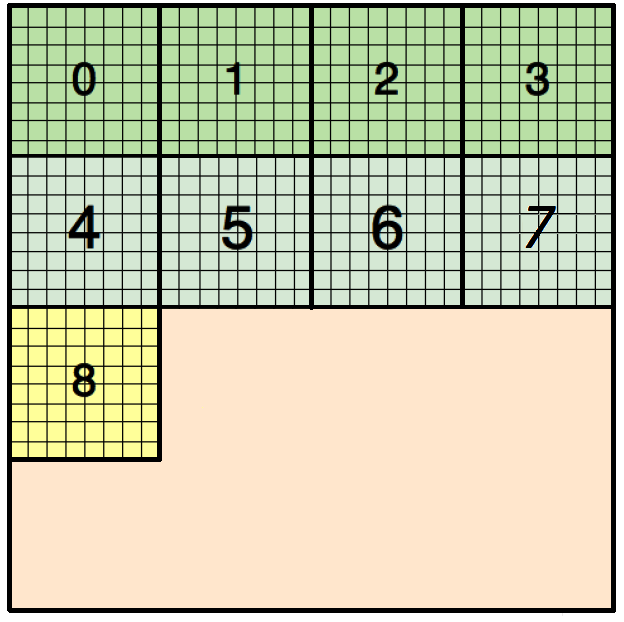
\includegraphics[width=0.3\textwidth]{Immagini/block_on_grid.png}
	\caption{Figura con singola immagine}
	\label{fig:one}
\end{figure}

\begin{figure}[ht]
	\centering
	\begin{subfigure}{0.3\textwidth}
		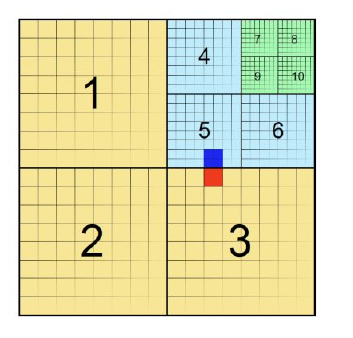
\includegraphics[width=1.0\textwidth]{Immagini/disoposizione_blocchi_fisica.png}
		\caption{Disposizione fisica dei blocchi}
	\end{subfigure}%
	\begin{subfigure}{0.3\textwidth}
		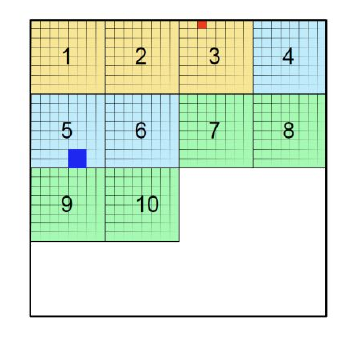
\includegraphics[width=1.0\textwidth]{Immagini/disoposizione_blocchi_logica.png}
		\caption{Disposizione logica dei blocchi}
	\end{subfigure}
	\caption{Figura con due immagini}
	\label{fig:two}
\end{figure}


\begin{figure}[H]
	\centering
	\begin{subfigure}{0.5\textwidth}
		\centering
		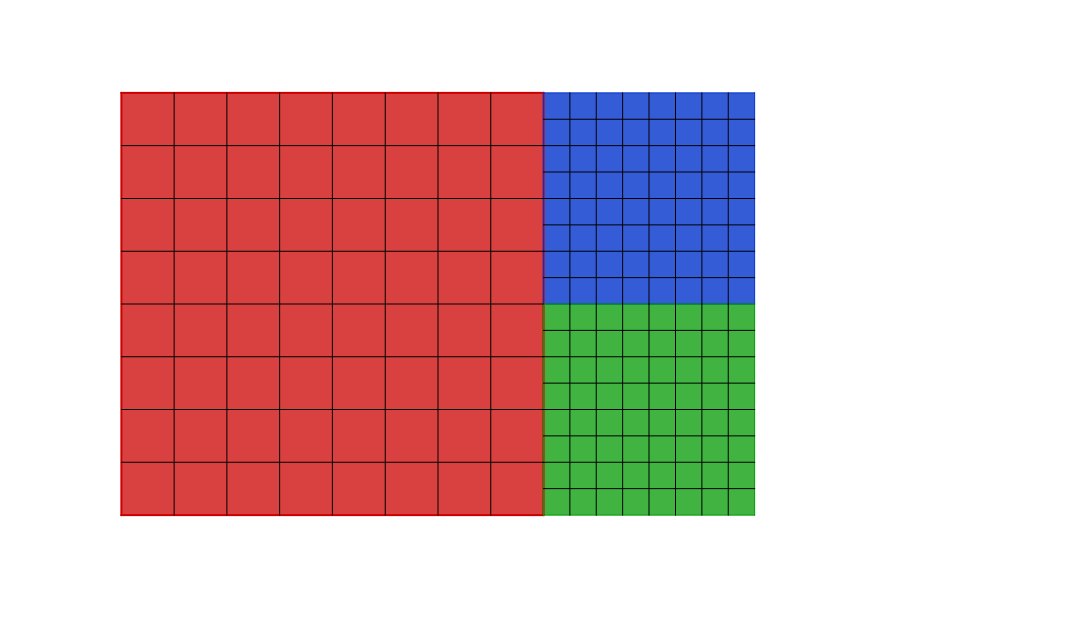
\includegraphics[width=0.7\linewidth]{Immagini/lev_less1.png}
		\caption{\textit{lev} = -1\newline}
		\label{fig:test1}
	\end{subfigure}%
	\begin{subfigure}{0.5\textwidth}
		\centering
		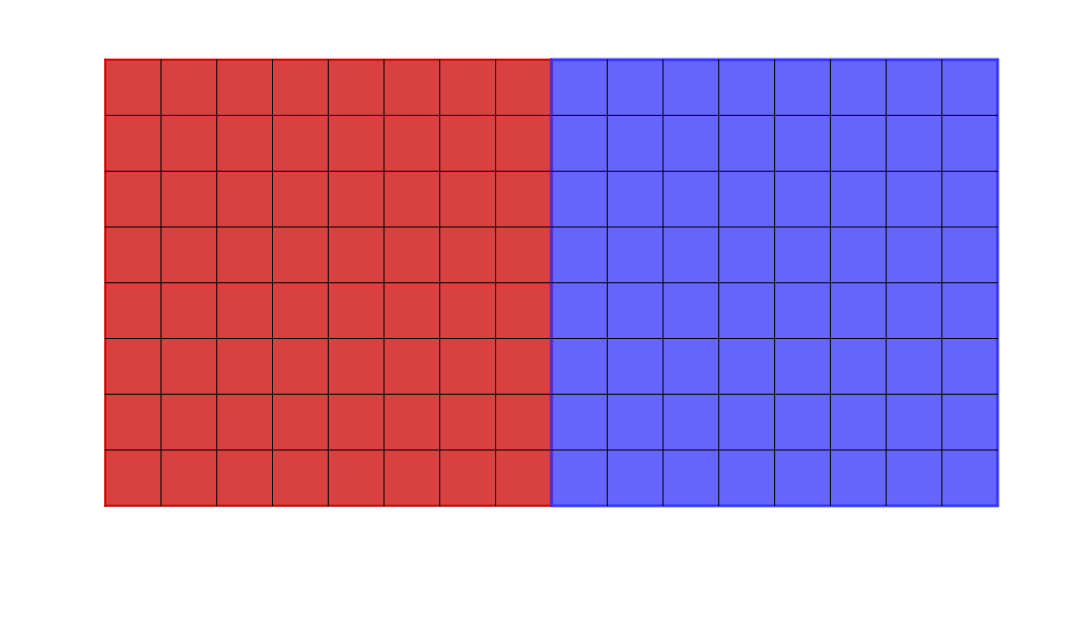
\includegraphics[width=0.7\linewidth]{Immagini/lev0.png}
		\caption{\textit{lev} = 0\newline}
		\label{fig:test2}
	\end{subfigure}
	\begin{subfigure}{0.7\textwidth}
		\centering
		\begin{subfigure}{0.5\textwidth}
			\centering
			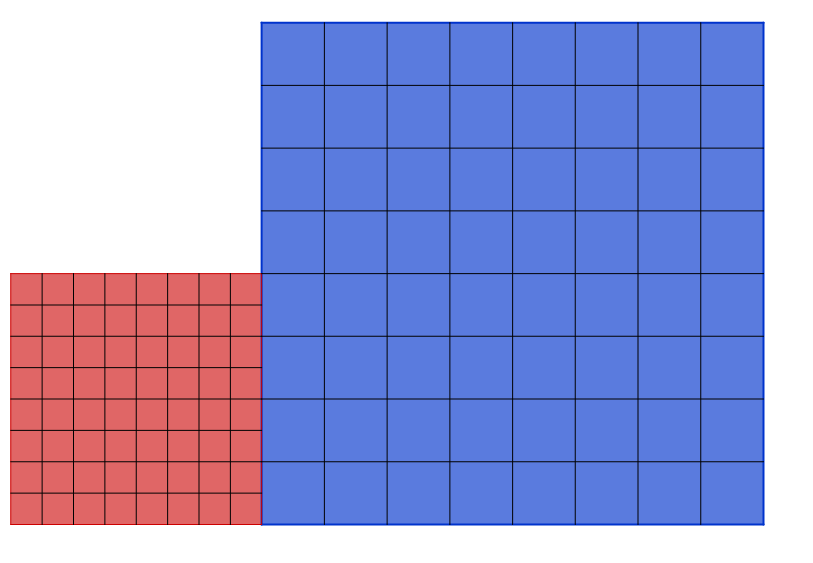
\includegraphics[width=0.5\linewidth]{Immagini/bloccomaggiore1.png}
		\end{subfigure}%
		\begin{subfigure}{0.5\textwidth}
			\centering
			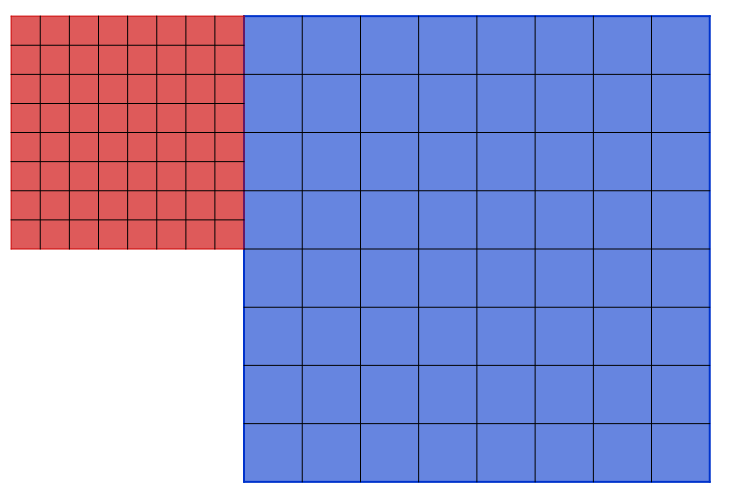
\includegraphics[width=0.5\linewidth]{Immagini/bloccomaggiore2.png}
		\end{subfigure}
		\caption{\textit{lev} = 1}
		\label{fig:lev1}
	\end{subfigure}
	\caption{Figura con tre immagini (di cui una composta da due sotto-immagini)}
	\label{fig:three}
\end{figure}

\section{Esempi di Codice e Misc.}\label{sec:code}
Alcuni esempi di codice, definizioni, tabelle e altro.

\begin{algorithm}[ht]
	\caption{Esempio di pseudo-codice}
	\label{alg:Prim_Mst}
	\begin{algorithmic}[1]
		\Statex
		\Function{MST-Prim}{grafo G, funzione\_peso $\omega$, nodo\_radice r}\\
		\State{\textit{Q}: coda di priorita contenente tutti i vertici in \textit{V}}
		\For{ogni \textit{u} $\in$ V(G)}
		\Let{\textit{u.key}}{$\infty$}
		\Let{\textit{u.}$\pi$}{\textit{NIL}} 
		\EndFor
		\Let{\textit{r.key}}{0}
		\Let{\textit{Q}}{\textit{V(G)}}
		\While{\textit{Q} $\neq$ 0}
		\Let{\textit{u}}{EXTRACT-MIN(\textit{Q})}
		\For{ogni \textit{v} $\in$ \textit{G.Adj[u]}}
		\If{$v \in Q$ and $\omega(u,v) < v.key$}
		\Let{\textit{v.key}}{$\omega(u,v)$}
		\Let{\textit{v.}$\pi$}{\textit{v}}
		\EndIf
		\EndFor
		\EndWhile
		\State \Return{}
		\EndFunction
	\end{algorithmic}
\end{algorithm}

\begin{minipage}{\textwidth}
\begin{lstlisting}[caption={Esempio di definizione struttura dati C++, ma non algoritmo},
	label={lst:block_struct}]
	struct Block
	{
		int id_block;
		char resolution;
		int id_subdomain;
		int key;
		bool in_other_subdomain;
		struct neigh_t neighbors[4];
	};
\end{lstlisting}
\end{minipage}



\begin{algorithm}[ht]
	\caption{Esempio di codice imperativo}
	\label{alg:my_prim_multi}
	\begin{algorithmic}[1]
		\Statex
		\Function{PRIM\_MULTI-MST}{roots\_list \textit{roots}, array\_Block \textit{adjacency\_list}}
		
		\State{\color{blue}{//Inizializzazione di tutti i vertici}}
		\For{ogni \textit{u} $\in$ \textit{adjacency\_list}}
		\Let{\textit{u.key}}{$\infty$}
		\Let{\textit{u.id\_subdomains}}{\textit{NIL}}
		\Let{\textit{u.in\_other\_subdomain}}{FALSE} 
		\EndFor
		
		\State{\color{blue}{//Inizializzazione di tutte le radici}}
		\Let{\textit{i}}{0}
		\For{ogni \textit{r} $\in$ \textit{roots}}
		\Let{\textit{r.key}}{0}
		\Let{\textit{r.id\_subdomains}}{\textit{i}}
		\Let{\textit{i}}{$i+1$}
		\EndFor
		\State{\textit{Q}: coda di priorita ordinata in base al campo 
			\textit{key}}
		\Let{\textit{Q}}{\textit{roots}}
		\Let{\textit{count}}{0}
		
		\While{count $<$ \textit{adjacency\_list.size}}
		\Let{\textit{u}}{EXTRACT-MIN(\textit{Q})}
		
		\If{!(\textit{u.in\_other\_subdomain})}
		\State{\color{blue}{//Essendo il minimo viene aggiunto definitivamente}}
		\Let{\textit{u.in\_other\_subdomain}}{TRUE}
		\State{\color{blue}{//Si analizzano i vicini}}
		\For{ogni \textit{v} $\in$ \textit{u.neighbors}}
		\State{\color{blue}{//In questo caso specifico il peso di ogni arco vale 1}}
		\If{$v \in adjacency\_list$ and ($u.key+1) < v.key$}
		\Let{\textit{v.key}}{$u.key+1$}
		\Let{\textit{v.subdomains}}{\textit{u.subdomains}}
		\Let{\textit{count}}{\textit{count} + 1}
		\EndIf
		\EndFor
		\EndIf
		\EndWhile
		\State \Return{}
		\EndFunction
	\end{algorithmic}
\end{algorithm}

\begin{algorithm}[ht]
	\caption{esempio di algoritmo in C++}
	\label{lst:genic_mpi}
	\begin{lstlisting}
		#include (*@\textquotedblleft@*)mpi.h"
		
		(*@~ ~ ~ ~\raisebox{-1pt}[0pt][0pt]{$\vdots$}@*)
		
		main(int argc, char** argv){
			
			(*@~ ~ ~ ~ ~ ~ ~ ~ ~ ~{\raisebox{-1pt}[0pt][0pt]{$\vdots$}}@*)
			
			//Nessuna chiamata a funzioni MPI prima di questa
			MPI_Init(&argc, &argv);
			
			(*@~ ~ ~ ~ ~ ~ ~ ~ ~ ~{\raisebox{-1pt}[0pt][0pt]{$\vdots$}}@*)
			
			MPI_Finalize();
			//Nessuna chiamata a funzioni MPI dopo questa
			
			(*@~ ~ ~ ~ ~ ~ ~ ~ ~ ~{\raisebox{-1pt}[0pt][0pt]{$\vdots$}}@*)
		}	
	\end{lstlisting}
\end{algorithm}

\begin{defn}[Esempio di Definizione]
	Un piccolo esempio di definizione
\end{defn}

\begin{table}[ht]
	\centering
	\resizebox{0.99\linewidth}{!}{
		\begin{tabular}{||c||c|c|c|c|c|c|c|c|c|c||}
			\hhline{|t:=:t:==========:t|}
			CT scan &\phantom{00}01\phantom{00}&\phantom{00}02\phantom{00}&\phantom{00}03\phantom{00}&\phantom{00}04\phantom{00}&\phantom{00}05&\phantom{00}06\phantom{00}&\phantom{00}07\phantom{00}&\phantom{00}08\phantom{00}&\phantom{00}09\phantom{00}&\phantom{00}10\phantom{00} \\
			\hhline{|:=::==========:|}
			Input arteries (n.) &66&175&76&134&198&172&154&108&91&65 \\
			\hhline{||-||----------||}
			Labeling time (s)&19.13&87.38&26.11&47.08&90.89&356.95&303.77&91.95&16.01&21.88 \\
			\hhline{||-||----------||}
			Grounding time (s)&9.76&52.45&9.57&22.88&70.34&47.52&37.44&17.98&10.61&8.04 \\
			\hhline{||-||----------||}
			Optimum time (s)&6.66&31.05&14.67&20.63&15.2&29.17&54.71&61.03&4.28&7.24 \\
			\hhline{|b:=:b:==========:b|}
		\end{tabular}
	}
	\vspace*{2mm}
	\caption{Esempio di tabella}
	\label{tab:perf}
\end{table}


\section{Citazioni}
Durante la scrittura della Tesi è necessario fornire i riferimenti bibliografici che hanno permesso la stesura della tesi stessa.
Questo si ottiene semplicemente tramite l'utilizzo del comando ``cite'' che prende come argomento la label di una delle entry nel file .bib.
Quindi per citare una qualunque fonte, ad esempio ``Artificial Intelligence - A Modern Approach", si può fare \cite{modernApproach} ($\backslash\text{cite}\{\text{modernApproach}\}$).
Questo leggerà la referenza nel file .bib che ha come label ``cormen".
Per citare più riferimenti contemporaneamente basta sperare le varie labels con una virgola come segue \cite{gelfond1998action,modernApproach,durfee1999distributed,de2003resource,allen2009complexity,bernstein2002complexity}.
Le reference non citate non appariranno in bibliografia.
\href{https://dblp.uni-trier.de/}{dblp} e \href{https://scholar.google.com/}{Google Scholar} sono siti nei quali estrarre la reference per bibtex per un lavoro di cui si conosce solo il titolo, ad esempio.
\chapter{Background}\label{chapter:background}
\section{Teoria degli insiemi}
\begin{definition}[Insieme]
Un \textit{insieme} è una collezione di elementi. Lo si può descrivere in due modi: 
\begin{itemize}
    \item estensionalmente: come elenco degli elementi presenti nell'insieme separati da virgole e contenuti tra parentesi graffe;
    \item per proprietà caratteristica: come l'insieme di oggetti che soddisfano una proprietà P, con questa sintassi \(\{x\ |\ \textrm{P}(x)\}\);
\end{itemize}
\end{definition}

\begin{definition}[Appartenenza]
Se un elemento \(x\) fa parte di un insieme \(X\) diremo che \(x\) \textit{appartiene} ad \(X\) e scriviamo \(x\in X\), altrimenti \(x \notin X\).
\end{definition}

\begin{definition}[Cardinalità]
La \textit{cardinalità} di un insieme \(X\) è il numero di elementi al suo interno e lo si denota con \(|X|\). Un insieme può avere un numero infinito di elementi. Un insieme con cardinalità 0 è detto \textit{insieme vuoto} e viene rappresentato con \(\{\}\) oppure \(\emptyset\).
\end{definition}

\begin{definition}[Operazioni sugli insiemi]
Esistono numerose operazioni applicabili agli insiemi, le principali sono:
\begin{itemize}
    \item \textit{unione}: l'unione di due insiemi \(A, B\) si scrive \(A\cup B\) e deonota l'insieme contenente tutti gli elementi di \(A\) o di \(B\) o di entrambi;
    \item \textit{intersezione}: l'intersezione di due insiemi \(A, B\) si scrive \(A\cap B\) e deonota l'insieme contenente tutti gli elementi presenti sia in \(A\) che in \(B\);
    \item \textit{differenza}: la differenza tra un insieme \(A\) ed un insieme \(B\) si scrive \(A\setminus B\) e deonota l'insieme contenente tutti gli elementi di \(A\) non presenti in \(B\);
\end{itemize}
\end{definition}

\begin{definition}[Relazioni tra insiemi]
Due insiemi \(A, B\) si dicono:
\begin{itemize}
    \item \textit{congiunti} se sono lo stesso insieme, ovvero se \(A\setminus B=B\setminus A=\emptyset\);
    \item \textit{disgiunti}  se non hanno elementi in comune, ovvero \(A\cap B=\emptyset\);
\end{itemize}
Si dice che \(B\) è \textit{sottoinsieme} di \(A\) se \(A\) contiene tutti gli elementi di \(B\) e si scrive \(B\subseteq A\). Se vogliamo escludere che \(B\) coincida con \(A\) scriviamo \(B\subset A\). 
\end{definition}

\begin{definition}[Insieme delle parti]
Dato un qualisasi insieme \(A\) si definisce \textit{insieme delle parti} l'insieme che contiene tutti e soli i sottoinsiemi di \(A\), lo denotiamo con \(\wp(A)=\{B\ |\ B\subseteq A\}\).
\end{definition}

\begin{definition}[Prodotto cartesiano]
Il \textit{prodotto cartesiano} degli insiemi \(X_1,X_2,\cdots,X_n\) è l'insieme di tutte le n-uple dove il primo elemento appartiene a \(X_1\), il secondo a \(X_2\) e così via. Formalmente si scrive \(X_1\times X_2\times\cdots\times X_n=\{\langle x_1, x_2,\cdots, x_n\rangle\ |\ x_1\in X_1\wedge x_2\in X_2\wedge\cdots\wedge x_n\in X_n\}\)
\end{definition}

\begin{definition}[Relazione]
Una \textit{relazione} R tra gli insiemi \(X_1,X_2,\cdots,X_n\) è un sottoinsieme del prodotto cartesiano \(X_1\times X_2\times\cdots\times X_n\). Gli elementi \(x_i\) con \(i\in [\, n]\) sono in relazione R se \(\langle x_1, x_2,\cdots, x_n\rangle\in\textrm{R}\). Un relazione \(\textrm{R}_b\) definita tra due insiemi \(X, Y\) si dice relazione binaria, se due elementi \(x, y\) sono in relazione \(\textrm{R}_b\) tra di loro scriveremo \(x\textrm{R}_b y\).
\end{definition}

\begin{definition}[Relazione di ordine parziale]
Una relazione binaria \(\preceq\) sull'insieme \(S\) è una \textit{relazione di ordine parziale} se possiede queste tre proprietà:
\begin{itemize}
\item Riflessività: \(\forall s\in S. s\preceq s\);
\item Antisimmetrica: \(\forall s_1, s_2\in S. s_1\preceq s_2 \wedge s_2\preceq s_1 \Rightarrow s_1=s_2\);
\item Transitività: \(\forall s_1, s_2, s_3 \in S. s_1\preceq s_2 \wedge s_2\preceq s_3 \Rightarrow s_1\preceq s_3\);
\end{itemize}
\end{definition}

\section{Teoria degli ordini}
\begin{definition}[Insieme parzialmente ordinato]
Un \textit{insieme parzialmente ordinato} (o poset) è una coppia \(\langle S, \preceq\rangle\) dove \(S\) è un insieme di elementi e \(\preceq\) è una relazione di ordine parziale su \(S\).
\end{definition}

\begin{definition}[Catena]
Una catena di un poset \(\simplePoset{S}\) è un sottoinsieme \(C\subseteq S\) tale che: \(\forall c_1, c_2 \in C. c_1\preceq_{S} c_2 \vee c_2\preceq_{S} c_1\)
\end{definition}

\begin{definition}[Copertura]
Dato un poset \(\simplePoset{S}\) e due elementi \(s_1, s_2 \in S\) diciamo che \(s_1\) \textit{copre} \(s_2\) se non esiste un altro elemento \(s_3\in S\) tale che \(s_1 \preceq_{S} s_3 \preceq_{S} s_2\).
\end{definition}

\begin{definition}[Diagramma di Hasse]
\'E possibile visualizzare un insieme parzialmente ordinato \(\simplePoset{S}\) attraverso un \textit{diagramma di Hasse}. Un diagramma di Hasse è un grafo i cui nodi sono gli elementi dell'isnsieme \(S\) del poset e un arco viene disegnato tra due elementi \(s_1, s_2 \in S\) solo se \(s_1\) copre \(s_2\).
\end{definition}

\begin{example} 
Se prendiamo l'insieme \(\textrm{Sign}=\{\perp, +, -, 0, 0+, 0-, \top\}\) e l'ordinamento parziale \(\preceq_{\textrm{Sign}}\) definito dal diagramma di Hasse in figura \ref{fig:signDomain} allora \(\simplePoset{\textrm{Sign}}\) è un insieme parzialmente ordinato.

\begin{figure}
\begin{center}
\begin{scriptsize}
\begin{tikzpicture}
[align=center,node distance=1.4cm]
\node [rectangle,draw=black!25] (top) {\(\top\)};
\node [rectangle,draw=black!25] (zeroplus) [below right of=top]{\(0+\)};
\node [rectangle,draw=black!25] (zerominus) [below left of=top]{\(0-\)};
\node [rectangle,draw=black!25] (zero) [below left of=zeroplus]{\(0\)};
\node [rectangle,draw=black!25] (plus) [below right of=zeroplus]{\(+\)};
\node [rectangle,draw=black!25] (minus) [below left of=zerominus]{\(-\)};
\node [rectangle,draw=black!25] (bottom) [below of=zero]{\(\perp\)};

\draw (top.270) -- (zeroplus.90);
\draw (top.270) -- (zerominus.90);
\draw (zerominus.270) -- (minus.90);
\draw (zeroplus.270) -- (plus.90);
\draw (zerominus.270) -- (zero.90);
\draw (zeroplus.270) -- (zero.90);
\draw (bottom.90) -- (plus.270);
\draw (bottom.90) -- (zero);
\draw (bottom.90) -- (minus.270);
\end{tikzpicture}
\end{scriptsize}
\end{center}
\caption{diagramma di Hasse del dominio dei segni.}
\label{fig:signDomain}
\end{figure}
\end{example}

\begin{definition}[Condizione di catena ascendnente]
Un poset \(\simplePoset{S}\) soddisfa la \textit{condizione di catena ascendnente} (ACC) se e solo se ogni sequenza infinita \(\emph{s}_0\preceq\emph{s}_1\preceq\cdots\preceq\emph{s}_k\preceq\cdots\) di elementi di \emph{S} se: \(\exists\emph{n}\in\mathbb{N}.\ \emph{s}_m=\emph{s}_n\forall\emph{m}\geq\emph{n}\).
\end{definition}

\begin{definition}[Condizione di catena discendnente]
Un poset \(\simplePoset{S}\) soddisfa la \textit{condizione di catena discendnente} (DCC) se e solo se ogni sequenza infinita \(\emph{s}_0\succeq\emph{s}_1\succeq\cdots\succeq\emph{s}_k\succeq\cdots\) di elementi di \emph{S} se: \(\exists\emph{n}\in\mathbb{N}.\ \emph{s}_m=\emph{s}_n\forall\emph{m}\geq\emph{n}\).
\end{definition}

\begin{definition}[Upper bound e lub]
Dato un poset \(\simplePoset{S}\) e \(X\subseteq S\), \emph{l} è l'\textit{upper bound} di \emph{X} se \(\forall x\in X. x\preceq l\). Se l'insieme degli upper bound di \emph{X} ha un minimo questo lo chiamiamo \textit{least upper bound} (lub) e lo si denota con \(\bigsqcup X\). Se abbiamo l'insieme \(X=\{x_1, x_2\}\) (cioè composto da due elementi) possiamo scrivere equivalentemente \(\bigsqcup X=x_1\sqcup x_2\).
\end{definition}

\begin{definition}[Lower bound e glb]
Dato un poset \(\simplePoset{S}\) e \(X\subseteq S\), \emph{g} è il \textit{lower bound} di \emph{X} se \(\forall x\in X. x\succeq g\). Se l'insieme dei lower bound di \emph{X} ha un massimo questo lo chiamiamo \textit{greatest lower bound} (glb) e lo si denota con \(\bigsqcap X\). Se abbiamo l'insieme \(X=\{x_1, x_2\}\) (cioè composto da due elementi) possiamo scrivere equivalentemente \(\bigsqcap X=x_1\sqcap x_2\).
\end{definition}

\begin{definition}[Insieme parzialmente ordinato completo]
Un poset \(\simplePoset{S}\) è \textit{completo} se ogni catena crescente \(C\subseteq S\) ha un least upper-bound in \(S\), ovvero \(\bigsqcup C \in S\).
\end{definition}

\begin{definition}[Top e bottom] 
Un elemento \(\emph{x}\in\emph{S}\) di un poset \(\simplePoset{S}\) è l'elemento \textit{top} \(\top\) se \(\forall\emph{y}\in\emph{S}.\emph{y}\preceq\emph{x}\). Mentre è l'elemento \textit{bottom} \(\perp\) se \(\forall\emph{y}\in\emph{S}.\emph{x}\preceq\emph{y}\).
\end{definition}

\begin{definition}[Join semi reticolo]
Un \textit{join semi reticolo} \(\langle S,\preceq_S, \sqcup\rangle\) è un poset \(\simplePoset{S}\) tale che \(\forall x, y\in S\) esiste il lub \(x\sqcup y\).
\end{definition}

\begin{definition}[Meet semi reticolo]
Un \textit{meet semi reticolo} \(\langle\emph{S },\preceq_S, \sqcap\rangle\) è un poset \(\simplePoset{S}\) tale che \(\forall x, y\in S\) esiste il glb \(x\sqcap y\).
\end{definition}

\begin{definition}[Reticolo]
Un \textit{reticolo} \(\simpleLattice{S}\) è sia un join semi reticolo che un meet semi reticolo.
\end{definition}

\begin{definition}[Reticolo completo]
Un reticolo \(\simpleLattice{S}\) è un \textit{reticolo completo} se: \(\forall D\subseteq S.\bigsqcup D,\bigsqcap D\in S\). Una conseguenza di ciò è che esistono gli elementi top e bottom. Per questo possiamo scrivere un reticolo completo come \(\completeLattice{S}\).
\end{definition}

\begin{example}
Dato un insieme \(A\) non vuoto qualsiasi \(\langle\wp(A), \subseteq, \cup, \cap, A, \emptyset\rangle\) è un reticolo completo.
\end{example}

\begin{example}
Mostriamo un'altro esempio di reticolo completo. Il dominio del reticolo è l'insieme:
\[\textrm{Int}=\{[l, u]\ |\ l, u\in\mathbb{Z} \wedge l\leq u\} \cup \{[-\infty, u]\ |\ u\in\mathbb{Z}\} \cup \{[l, +\infty]\ |\ l\in\mathbb{Z}\} \cup \{\perp, \top\}\]
l'elemento \(\top\) equivale a \([-\infty, +\infty]\) e l'elemento \(\perp\) all'insieme vuoto [ ].
La relazione di ordine parziale \(\preceq\) è così definita: per ogni \([l_1, u_1], [l_2, u_2]\in\textrm{Int}\) si ha che \([l_1, u_1]\preceq_{\textrm{Int}} [l_2, u_2]\) se e solo se \(l_2\leq l_1 \wedge u_1\leq u_2\). Infine definiamo un operatore di lub \(\sqcup\) e di glb \(\sqcap\) così: per ogni \([l_1, u_1], [l_2, u_2]\in\textrm{Int}\) si ha che 
\begin{itemize}
\item \([l_1, u_1]\sqcup [l_2, u_2] = [\textrm{min}(l_1, l_2), \textrm{max}(u_1, u_2)]\)
\item \([l_1, u_1]\sqcap [l_2, u_2] = \) 
	$
	\begin{cases}
	[l_1, u_1] & \textrm{se } [l_1, u_1]\preceq [l_2, u_2] \\
	[l_2, u_2] & \textrm{se } [l_2, u_2]\preceq [l_1, u_1] \\
	\perp      & \textrm{se } (u_1 < l_2 \wedge l_1 < l_2) \vee (u_2 < l_1 \wedge l_2 < l_1) \\
	[l_2, u_1] & \textrm{se } l_1<l_2\leq u_1 \wedge l_2\leq u_1<u_2 \\
	[l_1, u_2] & \textrm{se } l_2<l_1\leq u_2 \wedge l_1\leq u_1<u_1
	\end{cases} 
	$
 
    questo significa semplicemente che dobbiamo prendere l'intersezione dei due intervalli e se l'intersezione è nulla restituiamo \(\perp\).
\end{itemize}
Abbiamo quindi un reticolo completo \(\langle\textrm{Int}, \preceq_{\textrm{Int}}, \sqcup, \sqcap, [-\infty, +\infty], [\ ] \rangle\). In oltre è possibile visualizzare l'ordinamento parziale sull'insieme Int attraverso il diagramma di Hasse (ovviamente incompleto) in figura \ref{fig:intervalDomain} :

\begin{figure}
\begin{center}
\begin{scriptsize}
\begin{tikzpicture}
[align=center,node distance=1.4cm]
\node [rectangle,draw=black!25] (top) {\([-\infty, +\infty]\)};

\node [rectangle,draw=black!25] (minusInfto2) [below left of=top] {\([-\infty, 2]\)};
\node [rectangle,draw=black!25] (minusInfto1) [below left of=minusInfto2] {\([-\infty, 1]\)};
\node [rectangle,draw=black!25] (minusInftozero) [below left of=minusInfto1] {\([-\infty, 0]\)};
\node [rectangle,draw=black!25] (minusInftominus1) [below left of=minusInftozero] {\([-\infty, -1]\)};
\node [rectangle,draw=black!25] (minusInftominus2) [below left of=minusInftominus1] {\([-\infty, -2]\)};

\node [rectangle,draw=black!25] (minus2toInf) [below right of=top] {\([-2, +\infty]\)};
\node [rectangle,draw=black!25] (minus1toInf) [below right of=minus2toInf] {\([-1, +\infty]\)};
\node [rectangle,draw=black!25] (zerotoInf) [below right of=minus1toInf] {\([0, +\infty]\)};
\node [rectangle,draw=black!25] (plus1toInf) [below right of=zerotoInf] {\([1, +\infty]\)};
\node [rectangle,draw=black!25] (plus2toInf) [below right of=plus1toInf] {\([2, +\infty]\)};

\node [rectangle,draw=black!25] (minus2to2) [below left of=minus2toInf] {\([-2, 2]\)};
\node [rectangle,draw=black!25] (minus2to1) [below left of=minus2to2] {\([-2, 1]\)};
\node [rectangle,draw=black!25] (minus1to2) [below right of=minus2to2] {\([-1, 2]\)};

\node [rectangle,draw=black!25] (minus1to1) [below right of=minus2to1] {\([-1, 1]\)};
\node [rectangle,draw=black!25] (minus2tozero) [below left of=minus2to1] {\([-2, 0]\)};
\node [rectangle,draw=black!25] (zeroto2) [below right of=minus1to2] {\([0, 2]\)};

\node [rectangle,draw=black!25] (zeroto1) [below right of=minus1to1] {\([0, 1]\)};
\node [rectangle,draw=black!25] (minus1tozero) [below left of=minus1to1] {\([-1, 0]\)};
\node [rectangle,draw=black!25] (plus1to2) [below right of=zeroto2] {\([1, 2]\)};
\node [rectangle,draw=black!25] (minus2tominus1) [below left of=minus2tozero] {\([-2, -1]\)};

\node [rectangle,draw=black!25] (minus2) [below left of=minus2tominus1] {\([-2, -2]\)};
\node [rectangle,draw=black!25](minus1) [below left of=minus1tozero] {\([-1, -1]\)};
\node [rectangle,draw=black!25](zero) [below left of=zeroto1] {\([0, 0]\)};
\node [rectangle,draw=black!25] (plus1) [below left of=plus1to2] {\([1, 1]\)};
\node [rectangle,draw=black!25] (plus2) [below right of=plus1to2] {\([2, 2]\)};

\node [rectangle,draw=black!25] (bottom) [below of=zero] {\(\perp\)};

\node (minusdots) [left of=minus2] {\(\cdots\)};
\node (plusdots) [right of=plus2] {\(\cdots\)};


\draw (bottom.90) -- (zero.270);
\draw (bottom.90) -- (plus1.270);
\draw (bottom.90) -- (plus2.270);
\draw (bottom.90) -- (minus2.270);
\draw (bottom.90) -- (minus1.270);
\draw[dotted] (bottom.90) -- (plusdots.270);
\draw[dotted] (bottom.90) -- (minusdots.270);

\draw (zero.90) -- (minus1tozero.270);
\draw (zero.90) -- (zeroto1.270);
\draw (plus1.90) -- (plus1to2.270);
\draw (plus1.90) -- (zeroto1.270);
\draw (minus1.90) -- (minus1tozero.270);
\draw (minus1.90) -- (minus2tominus1.270);
\draw (minus2.90) -- (minus2tominus1.270);
\draw (plus2.90) -- (plus1to2.270);

\draw (minus2tominus1.90) -- (minus2tozero.270);
\draw (minus1tozero.90) -- (minus2tozero.270);
\draw (minus1tozero.90) -- (minus1to1.270);
\draw (zeroto1.90) -- (minus1to1.270);
\draw (zeroto1.90) -- (zeroto2.270);
\draw (plus1to2.90) -- (zeroto2.270);

\draw (minus1to1.90) -- (minus2to1.270);
\draw (minus1to1.90) -- (minus1to2.270);
\draw (minus2tozero.90) -- (minus2to1.270);
\draw (zeroto2.90) -- (minus1to2.270);

\draw (minus2to1.90) -- (minus2to2.270);
\draw (minus1to2.90) -- (minus2to2.270);

\draw (minusInftominus2.90) -- (minusInftominus1.270);
\draw (minusInftominus1.90) -- (minusInftozero.270);
\draw (minusInftozero.90) -- (minusInfto1.270);
\draw (minusInfto1.90) -- (minusInfto2.270);

\draw (plus2toInf.90) -- (plus1toInf.270);
\draw (plus1toInf.90) -- (zerotoInf.270);
\draw (zerotoInf.90) -- (minus1toInf.270);
\draw (minus1toInf.90) -- (minus2toInf.270);

\draw[dotted] (minus2.90) -- (minusInftominus2.270);
\draw[dotted] (minus2tominus1.90) -- (minusInftominus1.270);
\draw[dotted] (minus2tozero.90) -- (minusInftozero.270);
\draw[dotted] (minus2to1.90) -- (minusInfto1.270);
\draw[dotted] (minus2to2.90) -- (minusInfto2.270);

\draw[dotted] (plus2.90) -- (plus2toInf.270);
\draw[dotted] (plus1to2.90) -- (plus1toInf.270);
\draw[dotted] (zeroto2.90) -- (zerotoInf.270);
\draw[dotted] (minus1to2.90) -- (minus1toInf.270);
\draw[dotted] (minus2to2.90) -- (minus2toInf.270);

\draw[dotted] (minusInfto2.90) -- (top.270);
\draw[dotted] (minus2toInf.90) -- (top.270);

\end{tikzpicture}
\end{scriptsize}
\end{center}
\caption{rappresentazione incompleta del diagramma Hasse del dominio degli intervalli interi}
\label{fig:intervalDomain}
\end{figure}

Si può osservare come questo ordinamento non rispetta ne la condizione di catena ascendente ne la condizione di catena discendente.
\end{example}

\begin{definition}[Funzione parziale]
Una \textit{funzione parziale} \(f\) da \(A\) a \(B\), denotata \(f:A\rightharpoonup B\), è un sottoinsieme del prodotto cartesiano \(A\times B\) che associa ogni un elemento di \(A\) ad al massimo un elemento di \(B\). Scriviamo \(f(x)=y\) se la coppia \(\langle x, y\rangle\in f\). Definiamo il \textit{dominio} di una funzione parziale \(f:A\rightharpoonup B\) così: \(\textrm{dom}(f)=\{x\in A\ |\ \exists y\in B:f(x)=y\}\). L'insieme di tutte le funzioni parziali da \(A\) a \(B\) si scrive \(A\rightharpoonup B\).
\end{definition}

\begin{definition}[Funzione totale]
Una \textit{funzione totale} \(f\) da \(A\) a \(B\), denotata \(f:A\rightarrow B\), è una funzione parziale che associa ad ogni elemento di \(A\) esattamente un elemento di \(B\). Ovvero \(\textrm{dom}(f)=A\). L'insieme di tutte le funzioni totali si scrive \(A\rightarrow B\).
\end{definition}

\begin{definition}[Proprietà di una funzione]
Una funzione \(f:A\rightarrow B\) può essere:
\begin{itemize}
    \item \textit{suriettiva} se \(\forall y\in B : \exists x\in A: f(x)=y\);
    \item \textit{iniettiva} se \(\forall x,y\in A : f(x)=f(y)\Rightarrow x=y\);
    \item \textit{biiettiva} se è sia suriettiva che iniettiva;
\end{itemize}
Dati due poset \(\simplePoset{A}\) e \(\simplePoset{B}\) una funzione \(f:A\rightarrow B\) è detta:
\begin{itemize}
    \item \textit{monotona} se \(\forall x,y\in A, x\preceq_A y\Rightarrow f(x)\preceq_B f(y)\);
    \item \textit{continua} (o \textit{Scott-continua}) se per ogni catena \(C\subseteq A\), se \(\bigsqcup C\) esiste allora \(f(\bigsqcup C)=\bigsqcup\{f(x)\ |\ x\in C\}\);
    \item \textit{cocontinua} (o \textit{Scott-cocontinua}) se per ogni catena \(C\subseteq A\), se \(\bigsqcap C\) esiste allora \(f(\bigsqcap C)=\bigsqcap\{f(x)\ |\ x\in C\}\);
\end{itemize}
\end{definition}

\section{Teoria del fix-point}

\begin{definition}[Fix-point, pre-fix-point, post-fix-point]
Dato un \(\simplePoset{S}\) ed una funzione \(f:S\rightarrow S\) possiamo definire:
\begin{itemize}
\setlength\itemsep{0em}
	\item i fixpoint di \emph{f} quegli elementi \(s\in S\) tali che \(f(s)=s\), denotati con \(\textrm{fp}(f)\).
	\item i pre-fixpoint di \emph{f} quegli elementi \(s\in S\) tali che \(s\preceq_S f(s)\), denotati con \(\textrm{prefp}(f)\).
	\item i post-fixpoint di \emph{f} quegli elementi \(s\in S\) tali che \(f(s)\preceq_S s\), denotati con \(\textrm{postfp}(f)\).
\end{itemize}
\end{definition}

\begin{definition}[least fix-point, greatest fix-point]
Dato un \(\simplePoset{S}\) ed una funzione \(f:S\rightarrow S\) il \textit{least fix-point} di \textit{f}, scritto \(\textrm{lfp}(f)\), è un fix-point di \textit{f} tale che \(\forall x\in\textrm{fp}(f):\textrm{lfp}(f)\preceq_S x\). Dualmente il \textit{greatest fix-point} di \textit{f}, \(\textrm{gfp}(f)\), è un fix-point di \textit{f} tale che \(\forall x\in\textrm{fp}(f):x\preceq_S \textrm{gfp}(f)\).
\end{definition}

\begin{theorem}[Teorema del fix-point di Tarski]
Dato un reticolo completo \(\completeLattice{S}\) ed una funzione monotona \(f:S\rightarrow S\), anche l'insieme dei fix-point di f è un reticolo completo. 
\end{theorem}

Questo teorema garantisce l'esistenza di fix-point, e più in particolare garantisce l'esistenza di un least fix-point, \(\textrm{lfp}(f)=\bigsqcap\textrm{postfp}(f)\), e di un greatest fix-point, \(\textrm{gfp}(f)=\bigsqcup\textrm{prefp}(f)\). Il teorema non da però un metodo costruttivo per ottenere tali fix-point, per questo motivo c'è il teorema seguente.

\begin{theorem}[Teorema del fix-point di Kleene]
Dato un insieme parzialmente ordinato completo \(\simplePoset{S}\) ed una funzione Scott-continua \(f:S\rightarrow S\) allora f ha un least fix-point ed è il least upper bound della seguente catena crescente:
\[\perp\preceq_S f(\perp) \preceq_S f(f(\perp)) \preceq_S f(f(f(\perp))) \preceq_S \cdots\]
ovvero \(\textrm{lfp}(f)=\bigsqcup\{f^n(\perp)\ |\ n\geq 0\}\).
\end{theorem}

Più generalmente si può partire da qualsiasi pre-fix-point \(s\in S\) di \(f\) ottenendo \(\textrm{lfp}_s(f)=\bigsqcup\{f^n(s)\ |\ n\geq 0\}\) che è il più piccolo fix-point maggiore o uguale di \(s\).

\section{Connessione di Galois}

\begin{definition}[Connessione di Galois]
Dati due poset \(\simplePoset{A}\) e \(\simplePoset{C}\) e due funzioni \(\alpha:C\rightarrow A\) e \(\gamma:A\rightarrow C\), la quadrupla \(\langle \simplePoset{C}, \alpha, \gamma, \simplePoset{A}\rangle\) è una connessione di Galois (in corto dall'inglese GC) se e solo se:
\[\forall a\in A, \forall c\in C: \alpha(c)\preceq_A a \Leftrightarrow c\preceq_C \gamma(a)\]
Una GC \(\langle \simplePoset{C}, \alpha, \gamma, \simplePoset{A}\rangle\) si denota \(\simplePoset{C}\galois{\alpha}{\gamma}\simplePoset{A}\).
\end{definition}

Data una connessione di Galois \(\simplePoset{C}\galois{\alpha}{\gamma}\simplePoset{A}\) le funzioni \(\alpha\) e \(\gamma\) si determinano univocamente a vicenda in questo modo:
\[\alpha(c) = \bigsqcap_A\{a\ |\ c\preceq_C \gamma(a)\}\]
\[\gamma(a) = \bigsqcup_C\{c\ |\ \alpha(c)\preceq_A a\}\]

Un'altra importante proprietà delle connessioni di Galois è che date due connessioni di Galois \(\simplePoset{C}\galois{\alpha_1}{\gamma_1}\simplePoset{A}\) e \(\simplePoset{A}\galois{\alpha_2}{\gamma_2}\simplePoset{B}\), la loro composizione \(\simplePoset{C}\galois{\alpha_1\circ\alpha_2}{\gamma_1\circ\gamma_2}\simplePoset{B}\) è anche una connessione di Galois.

\begin{example}\label{ex:galoisSignInt}
Prendiamo i due poset mostrati negli esempi di prima, \(\simplePoset{\textrm{Int}}\) e \(\simplePoset{\textrm{Sign}}\), diamo una definizione delle funzioni \(\alpha:\textrm{Int}\rightarrow\textrm{Sign}\) e \(\gamma:\textrm{Sign}\rightarrow\textrm{Int}\) tali da creare la connessione di Galois \(\GaloisConnection{\textrm{Int}}{\textrm{Sign}}\):
\begin{itemize}
\item dato \(i\in\textrm{Int}\) abbiamo che \(\alpha(i)\) = 
$
\begin{cases}
\perp_{\textrm{Sign}}  & \textrm{se } i=\perp_{\textrm{Int}}\\
0  & \textrm{se } i=[0, 0]\\
+  & \textrm{se } i=[l, u], \textrm{con } l, u \in\mathbb{Z}^+\\
-  & \textrm{se } i=[l, u], \textrm{con } l, u \in\mathbb{Z}^-\\
0+  & \textrm{se } i=[0, u], \textrm{con } u \in\mathbb{Z}^+\\
0-  & \textrm{se } i=[l, 0], \textrm{con } l \in\mathbb{Z}^-\\
\top_{\textrm{Sign}}  & \textrm{se } i=[l, u], \textrm{con } l\in\mathbb{Z}^- \textrm{e } u \in\mathbb{Z}^+\\
\end{cases}
$
\item dato \(s\in\textrm{Sign}\) abbiamo che \(\gamma(s)\) =
$
\begin{cases}
\perp_{\textrm{Int}}  & \textrm{se } s=\perp_{\textrm{Sign}}\\
[0, 0] & \textrm{se } s=0 \\
[1, +\infty] & \textrm{se } s=+\\
[-\infty, -1] & \textrm{se } s=-\\
[0, +\infty] & \textrm{se } s=0+\\
[-\infty, 0] & \textrm{se } s=0-\\
[-\infty, +\infty] & \textrm{se } s=\top_{\textrm{Sign}}\\
\end{cases}
$

\end{itemize}
\end{example}

\begin{example}
Anche i poset \(\simplePoset{\textrm{Int}}\) e \(\langle\wp(\mathbb{Z}), \subseteq\rangle\) formano una connessione di Galois se definiamo \(\alpha:\wp(\mathbb{Z})\rightarrow\textrm{Int}\) e \(\gamma:\textrm{Int}\rightarrow\wp(\mathbb{Z})\) in questo modo:
\begin{itemize}
\item dato \(p\in\wp(\mathbb{Z})\) si ha che \(\alpha(p)\) = 
$
\begin{cases}
\perp_{\textrm{Int}} & \textrm{se } p=\emptyset\\
[\textrm{min}(p), \textrm{max}(p)] & \textrm{altrimenti}\\
\end{cases}
$
    \item dato \(i=[l, u]\in\textrm{Int}\) si ha che \(\gamma(i)=\{z\ |\ l\leq z \leq u\}\);
\end{itemize}
dove le funzioni \(\textrm{min},\textrm{max}:\wp(\mathbb{Z})\rightarrow\mathbb{Z}\cup\{-\infty, +\infty\}\) possono restituire anche più/meno infinito nel caso l'insieme non sia vuoto ma non abbia un massimo/minimo (quindi se cresce/decresce all'infinito).
\end{example}

\section{Analisi statica ed Interpretazione astratta}

Lo scopo dell'\textit{analisi statica} è quello di provare formalmente certe proprietà di un programma. Per essere definita statica una analisi deve avere la caratteristica di non eseguire il codice (in caso opposto l'analisi si dice \textit{dinamica}, un esempio è il tradizionale metodo di debug con test), o meglio di non eseguirlo nella sua forma concreta. L'\textit{interpretazione astratta} è un modello matematico che può essere utilizzato per compiere analisi statica. L'idea basilare è quella di astrarre la computazione su un dominio astratto e interpretare il codice muovendoci in uno spazio di oggetti astratti che approssimano il dominio concreto. Per fare ciò dobbiamo creare una semantica astratta, che ragiona nel mondo del dominio astratto, che sia \textit{sound} in rispetto alla semantica concreta, la quale invece ragiona su un dominio concreto. Il motivo per cui ci accontentiamo di una approssimazione è che spesso lavorare sul dominio concreto risulta impossibile a causa dei limiti della computazione o è estremamente costoso in termini di tempo. Ci basta perciò una soluzione approssimata, ma corretta, da cui si spera sia possibile verificare certe proprietà del programma analizzato.

\subsection{Interpretazione astratta}
Un linguaggio \(\mathbb{L}\) mette a disposizione una semantica, ovvero una descrizione formale e matematica del comportamento di un programma \(\rho\) scritto in \(\mathbb{L}\) partendo da uno stato iniziale (che può rappresentare la collezione di elementi di input di \(\rho\)). Da tale semantica si possono ottenere diverse \textit{semantiche concrete}, ovvero funzioni \(\textbf{S}:Program_\mathbb{L}\rightarrow \mathbb{C}\),  che prendono un programma \(\rho\) in \(\mathbb{L}\) e restituiscono un oggetto dell'insieme \(\mathbb{C}\), detto \textit{dominio semantico concreto}, che ci dice qualcosa sul comportamento di \(\rho\) e attraverso cui è pssibile verificarne crete proprietà. Una caratteristica necessaria di un dominio concreto è che deve essere parte di un reticolo completo, per semplicità scriveremo \(\simplePoset{\mathbb{C}}\). Due esempi di semantiche concrete sono:
\begin{itemize}
    \item \textit{trace semantics}: il dominio concreto \(\mathbb{C}\) di questa semantica è l'insieme delle parti di tutte le tracce di esecuzione possibili (anche quelle infinite) per ogni possibile programma scritto in \(\mathbb{L}\) per ogni possibile input di tale programma. Per traccia intendiamo una sequenza di stati e per stato intendiamo una coppia che comprende un punto di programma e uno stato della memoria (quindi lo stato rappresenta una fotografia della memoria in un dato istante). La trace semantics prenderò come input un porgramma \(\rho\) in \(\mathbb{L}\) e restituirà l'insieme comprendente tutte le tracce di esecuzione possibili per quel programma partendo dal set di tutti i possibili input. Questa semantica quindi vede il comportamento di un programma come un insieme di tracce. Avendo a disposizione questa semantica possiamo verificare numerose proprietà di un programma tra cui la liveness, la reachability ma anche la terminazione, basterebbe infatti mostrare che l'insieme di tracce possibili comprenda solo tracce finite. Dal famoso problema della terminazione formulato da Turing sappiamo però che tale verifica è impossibile.
    \item \textit{collecting semantics}: un'altra, ma meno precisa, semantica concreta è la collecting semantics. Il dominio \(\mathbb{C}\) di questa semantica è l'insieme di tutte le funzioni che mappano ogni punto di programma possibile a un insieme di stati della memoria (si noti che il concetto di stato della memoria può essere semplificato al concetto di environment, ovvero una mappa che associa ad ogni variabile del programma un valore). La collecting semantics è una funzione che associa ad ogni programma \(\rho\) in \(\mathbb{L}\) una funzione che mappa ogni punto di programma di \(\rho\) all'insieme di tutti gli stati della memoria atraversabili in quel punto (o nella visione semplificata è una funzione che associa ad ogni punto di programma tutti gli environment che possono passare per quel punto). In pratica la collecting semantics ci dice tutti gli stati possibili durante l'esecuzione del programma ignorando l'ordine temporale che li lega (per questo la trace semantics contiene più informazione, essa infatti non ignora la sequenzialità tra gli stati). Anche questa semantica risulta impossibile da calcolare, sia per motivi legati alla terminazione che per l'impossibilità di rappresentare certi elementi di \(\mathbb{C}\) su una macchina (si pensi ad esempio ad un programma con un ciclo infinito che possiede un punto di programma attraverso cui passano infiniti environemnt diversi). 
\end{itemize}

Tramite l'interpretazione astratta (abbreaviato in inglese \textit{AI}) vogliamo sopperire a tutti i problemi legati alla calcolabilità delle semantiche concrete. Per essere efficiace una \textit{AI} deve comprendere due cose: un \textit{dominio semantico astratto}, \(\simplePoset{\mathbb{A}}\) (anch'esso parte di un reticolo completo), e una \textit{semantica astratta}, ovvero una funzione \(\textbf{S}_{\mathbb{A}}:Program_\mathbb{L}\rightarrow \mathbb{A}\). Bisogna poi mostrare due ralaioni tra mondo concreto e mondo astratto: per primo un collegamento tra il dominino concreto e quello astratto tramite una connessione di Galois \(\GaloisConnection{\mathbb{C}}{\mathbb{A}}\) e poi una relazione di soundness tra le due funzioni semantiche, ovvero bisognerà dimostrare che per ogni \(\rho\in Program_{\mathbb{L}}\) vale che \(\alpha(\textbf{S}[\rho])\preceq_{\mathbb{A}}\textbf{S}_{\mathbb{A}}[\rho]\). Questo significa che il risultato dell'\textit{AI} di un programma deve almeno contenere tutte le proprietà vere del programma, ovvero deve essere una corretta approssimazione dell'analisi concreta. Lo scambio che andiamo a fare è quello di cedere precisione sull'analisi (con la clausola di rimanese sound) in cambio della possibilità di compiere l'analisi su una macchina in tempo finito. 

Il motivo per cui abbiamo introdotto molte nozioni legate al mondo degli insiemi parzialmente ordinati, reticoli e fix-point è che le funzioni semantiche, sia concreta che astratta, possono essere costruite in termini della ricerca del least fix-point di un operatore monotono. Ovvero avremo \(\mathbf{S}[\rho]=\textrm{lfp}(T_{\mathbb{C}})\) e \(\mathbf{S}_{\mathbb{A}}[\rho]=\textrm{lfp}(T_{\mathbb{A}})\) dove \(T_{\mathbb{C}}:\mathbb{C}\rightarrow \mathbb{C}\) e \(T_{\mathbb{A}}:\mathbb{A}\rightarrow \mathbb{A}\) sono operatori monotoni rispettivamente sul dominino concreto e su quello astratto. In questo caso la relazione di soundness tra le due semantica si appoggia sulla relazione di soundness tra i due operatori sottostanti seguendo la definizione seguente:

\iffalse
Dato un linguaggio \(\mathbb{L}\) ed un programma \(\rho\) scritto in \(\mathbb{L}\), la \textit{semantica} di \(\rho\) descrive l'insieme di tutti i possibili comportamenti di \(\rho\) quando eseguito per tutti i possibili valori di input. Dai risultati della semantica di \(\rho\) ne sarebbe possibile verificare molte proprietà riguardanti il suo comportamento run-time (come la terminazione o non-terminazione, l'impossibilità/possibilità o certezza di raggiungere certi stati e così via).

Generalmente partendo dal linguaggio \(\mathbb{L}\) è possibile creare una funzione semantica \(\textbf{S}:Program_\mathbb{L}\rightarrow \mathbb{C}\), detta \textit{semantica concreta}, che dato un programma scritto in \(\mathbb{L}\) ci restituisce un oggetto in \(\mathbb{C}\) rappresentabile proprio tutti i possibili comportamenti per tutti i possibili input di tale programma. L'insieme \(\mathbb{C}\), detto \textit{dominio semantico concreto} (e parte di un reticolo completo \(\CompleteLattice{\mathbb{C}}\)) è quindi l'insieme di tutti i possibili comportanti di tutti i possibili programmi in \(\mathbb{L}\). Il problema della semantica concreta è che spesso non è computabile, per problemi legati alla terminazione, o i suoi risultati non sono rappresentabili in una macchina, essendo il dominio concreto potenzialmento formato da elementi infiniti (si pensi a una traccia di esecuzione non terminante formata da una infinita sequenza di stati). E' comune il caso in cui la funzione semantica si basi sul calcolo del least fix-point di un operatore monotono \(T_{\mathbb{C}}:\mathbb{C}\rightarrow \mathbb{C}\), e quindi dato un programma \(\rho\) in \(\mathbb{L}\) si avrebbe \(\textbf{S}[\rho]=\textrm{lfp}(T_{\mathbb{C}})\).

Una interpretazione astratta deve essere dotata di due cose: un \textit{dominio semantico astratto} \(\mathbb{A}\) (anch'esso parte di un reticolo completo, \(\CompleteLattice{\mathbb{A}}\)) ed una funzione \textit{semantica astratta}, \(\textbf{S}_{\mathbb{A}}:Program_\mathbb{L}\rightarrow \mathbb{A}\) (o nel caso si tratti di una semantica concreta basata su calcolo del least fix-point serve una versione astratta dell'operatore monotono \(T_{\mathbb{C}}\), ovvero \(T_{\mathbb{A}}:\mathbb{A}\rightarrow \mathbb{A}\)).
Bisogna poi dimostrare il collegamento tra i due domini \(\mathbb{A}\) e \(\mathbb{C}\). Questo lo si fa tramite una connessione di Galois, ovvero trovando una coppia di funzioni monotone \(\alpha:\mathbb{C}\rightarrow \mathbb{A}\) e \(\gamma:\mathbb{A}\rightarrow \mathbb{C}\) con le proprietà precedentemente descritte che mostri che \(\mathbb{A}\) sia una corretta approssimazione di \(\mathbb{C}\). Infine affinchè l'interpretazione astratta sia corretta bisigna dimostrare la relazione di soundness tra la semantica concreta \(\textbf{S}\) e la semantica astratta \(\textbf{S}_{\mathbb{A}}\), ovvero bisogna mostrare che per ogni \(\rho\in Program_{\mathbb{L}}\) vale che \(\alpha(\textbf{S}[\rho])\preceq_{\mathbb{A}}\textbf{S}_{\mathbb{A}}[\rho]\). Se si sta invece lavorando su semantiche basate sul calcolo del least fix-point per dimostare la relazione di soundness basta verificare la seguente condizione sugli operatori monotoni sottostanti: \(\alpha\circ T_{\mathbb{C}}\preceq_{\mathbb{A}} T_{\mathbb{A}}\circ\alpha\), ovvero scritto in un altro modo bisogna mostrare che \(\forall c\in\mathbb{C}:\alpha(T_{\mathbb{C}}(c))\preceq_{\mathbb{A}}T_{\mathbb{A}}(\alpha(c))\).


Proviamo a darne una definizione più formale. Solitamente un linguaggio di programmazione imperativo L ci mette a disposizione una semantica operazionale che ci permette di eseguire un flusso computazionale di un programma \(p\) scritto in L. Da questa semantica e dal programma \(p\) si può ottenere una funzione \(f:\mathbb{C}\rightarrow\mathbb{C}\) che lavora su un dominio semantico concreto \(\langle\mathbb{C}, \preceq_{\mathbb{C}}\rangle\), dotato di un ordinamento parziale, i cui oggetti rappresentano certe proprietà di \(p\). Il limite o least fixed-point o risultato di \(f\) sarà un insieme di proprietà vere per \(p\). Come abbiamo già detto lavorare in questo universo di oggetti è di solito impossibile, infatti gli elementi di \(\mathbb{C}\) spesso rappresentano insiemi infiniti che non possono essere rappresentati su una macchina o sono il risultato di una computazione non terminante. Per questo ci spostiamo su un dominio astratto \(\langle\mathbb{A}, \preceq_{\mathbb{A}}\rangle\). Dalla stessa semantica operazionale e dallo stesso programma \(p\) si può ottenere un'altra funzione \(f^{\star}:\mathbb{A}\rightarrow\mathbb{A}\) che lavora sul dominio astratto e il cui limite o least fixed-point o risultato è una approssimazione corretta di \(f\), \(i.e.\), c'è una relazione di soundness tra \(f\) e \(f^{\star}\). Ovviamente il dominio astratto \(\mathbb{A}\) e la funzione \(f^{\star}\) vanno costruiti in modo tale da essere rappresentabili e calcolabili da un computer. Il limite di questo approccio è che ciò che è in grado di dirci \(f^{\star}\) su \(p\) potrebbe essere non è abbastanza preciso e raffinato per verificarne certe proprietà.
\fi

\begin{definition}[Soundness]
Prendiamo in considerazione due poset \(\simplePoset{C}, \simplePoset{A}\) che siano connessi tramite \(\simplePoset{C}\galois{\alpha}{\gamma}\simplePoset{A}\) e due funzioni \(f:C\rightarrow C\) e \(f^{\natural}:A\rightarrow A\) diremo che \(f^{\natural}\) è una approssimazione \textit{sound} di \(f\) se vale la seguente condizione:
\[\forall c\in C : \alpha(f(c))\preceq_A f^{\natural}(\alpha(c))\]
oppure equivalentemente:
\[\forall a\in A : f(\gamma(a)) \preceq_C \gamma(f^{\natural}(a))\]

Inoltre date tutte le approssimazioni di \(f\) esistenti vorremmo sapere quale è quella più precisa, quella che perde meno informazione ovvero vorremmo conoscere la \textit{migliore approssimazione corretta}. Date le ipotesi di sopra la funzione \(\alpha\circ f\circ\gamma:A\rightarrow A\) è la migliore approssimazione corretta.
\end{definition}



\subsection{Calcolo del fix-point}
Come già abbiamo detto spesso la semantica (sia astratta che concreta) viene espressa in termini di ricerca del least fix-point di un'altra funzione. Risulta molto utile, se non necessario, dare qualche definizione e teorema che ci permette di trasferire il calcolo del lfp di una funzione concreta \(f\) su una funzione astratta \(f^{\natural}\).

\begin{definition}[Fix-point soundness]
Data una connessione di Galois \(\GaloisConnection{C}{A}\), una funzione concreta \(f:C\rightarrow C\) ed una funzione astratta \(f^{\natural}:A\rightarrow A\) diciamo che \(f^{\natural}\) è \textit{fix-point sound} se \(\alpha(\textrm{lfp}(f))\preceq_A \textrm{lfp}(f^{\natural})\).
\end{definition}

\begin{theorem}[Approssimazione del fix-point]
Presi \(\GaloisConnection{C}{A}\), una funzione concreta \(f:C\rightarrow C\) ed una funzione astratta \(f^{\natural}:A\rightarrow A\) se \(\forall c\in C: \alpha(f(c))\preceq_A f^{\natural}(\alpha(c))\) allora \(f^{\natural}\) è fix-point sound, ovvero \(\alpha(\textrm{lfp}(f))\preceq_A \textrm{lfp}(f^{\natural})\).
\end{theorem}

\subsection{Interpretazione astratta di un Control Flow Graph}

Un Control Flow Graph (CFG) è una rappresentazione di un programma tramite una coppia \(\cfg\) dove \(N\) è un insieme di nodi, questi rappresentano blocchi di codice basilari del programma (ad esempio gli statement), e \(E\subset N\times N\) è l'insieme di archi che collegano i nodi in \(N\), questi rappresentano il flusso di informazione tra i blocchi. Gli archi possono essere sequenziali (l'informazione passa dal nodo di partenza a quello di arrivo sempre senza modifiche), veri (l'informazione passa solo se la condizione nel nodo di partenza è vera) o falsi (opposti agli archi veri). In questo modo possiamo rappresentare anche l'if statement all'interno del linguaggio CFG. Per rappresentare gli statement di loop basta creare dei cicli all'interno del CFG.

Dato un programma in CFG \(\cfg\) certe semantiche concrete possono essere espresse come il least fix-point del sistema di equazioni \(F:\mathbb{C}^{|N|}\rightarrow\mathbb{C}^{|N|}\) dove:
\[F = \{x_i = f_i(x_1, x_2, \cdots, x_{|N|})\ |\ i=1, 2,\cdots, |N|\}\]
in cui i vari \(f_i:\mathbb{C}^{|N|}\rightarrow\mathbb{C}\) sono funzioni trasformatrici concrete che simulano il comportamento del blocco di codice rappresentato dal nodo sulle informazioni provenienti dagli altri blocchi. La soluzione più piccola del sistema \(F\) sarà il least fix-point di \(F\), ovvero il least upper bound tra tutti gli step della iterazione di Kleene sul dominio concreto \(\mathbb{C}^{|N|}\) di \(F\) partendo dall'elemento bottom (in questo caso \(\perp_{\mathbb{C}}^{|N|}\)).

\begin{example}\label{ex:easyCode}
Nella figura \ref{fig:codiceEsempio1} si vede la traduzione di un semplice pezzo di codice scritto in Python in un CFG. 

\begin{figure}
\begin{minipage}{2cm}
\hspace{2cm}
\end{minipage}
\begin{minipage}[c][5cm][c]{0.5\textwidth-2cm}
\vspace{\fill}
\begin{lstlisting}[language=Python, numbers=none]
x = 0
if x < 10:
    x = x + 10
return x;
\end{lstlisting}
\vspace{\fill}
\end{minipage}
\begin{minipage}{0.5\textwidth}
\begin{center}
\begin{tikzpicture}
  [node distance=2cm, auto, 
  noline/.style={draw, -latex, draw=red!50, anchor=south, sloped}, 
  yesline/.style={draw, -latex, draw=blue!50, anchor=south, sloped}, 
  line/.style={draw, -latex, draw=black!25},
  block/.style={rectangle, draw=black!25}]
  % nodes
  \node [block] (init) {\(x = 0\)};
  \node [above left] at (init.north west) {\(x_1\)};
  \node [rectangle, draw=black!25, below of=init] (decide) {\(x < 10\)};
  \node [above left] at (decide.north west) {\(x_2\)};
  \node [rectangle, draw=black!25, below right of=decide] (then) {\(x = x + 10\)};
  \node [above right] at (then.north east) {\(x_3\)};
  \node [rectangle, draw=black!25, below left of=then] (end) {return \(x\);};
  \node [above left] at (end.north west) {\(x_4\)};

  % edges
  \path [line] (init) -- (decide);
  \path [yesline] (decide) -- node [above, font=\tiny] {True} (then);
  \path [line] (then) -- (end);
  \path [noline] (decide) --  node [below, font=\tiny] {False}  (end);

\end{tikzpicture}
\end{center}
\end{minipage}
\caption{}
\label{fig:codiceEsempio1}
\end{figure}

Supponiamo di usare come dominio semantico concreto l'insieme delle parti dei numeri interi che forma il reticolo \(\langle\wp(\mathbb{Z}), \cup, \cap, \emptyset, \mathbb{Z}\rangle\).
Il sistema di equazioni equivalente per trovare la collecting semantics è:
\[
F = 
\begin{cases}
   x_1 = \emptyset \\ 
   x_2 = \{0\} \\
   x_3 = \textrm{if}_{[x < 10]}(x_2) \\
   x_4 = \textrm{else}_{[x < 10]}(x_2) \cup (x_3 + \{10\}) \\
\end{cases}
\]

dove la funzione \(\textrm{if}_{[st]}:\wp(\mathbb{Z})\rightarrow\wp(\mathbb{Z})\) filtra i valori passati in input lasciando passare solo quelli che soddisfano la candizione in \(st\) (\(\textrm{else}_{[st]}:\wp(\mathbb{Z})\rightarrow\wp(\mathbb{Z})\) è simile ma fa passare solo quelli che non soddisfano la condizione \(st\)) e la funzione \(+:\wp(\mathbb{Z})\times\wp(\mathbb{Z})\rightarrow\wp(\mathbb{Z})\) somma elemento per elemento i valori dei due insiemi di interi passati come input. 

La collecting semantics sarà pari al least fix-point del sistema di equazioni \(F\) che è uguale al least upper bound tra tutti gli step della iterazione di Kleene (mostrata nel teorema [?]) di \(F\) su \(\wp(\mathbb{Z})^{|N|}\) partendo dal valore bottom di \(\wp(\mathbb{Z})\), ovvero \(\emptyset\), per ogni nodo.  

Per questo semplice esempio possiamo facilmente trovare il least fix-point. Partiamo da un vettore con tutti valori bottom:

\begin{figure}[H]
    \centering
\[
\arraycolsep=1.1pt
\begin{array}{ccccccccccc}
    \begin{tabular}{l}
    $
    t_0
    $ \\
    $
    \begin{bmatrix}
       \perp \\
       \perp \\
       \perp \\
       \perp
    \end{bmatrix}
    $
    \end{tabular}
    &
    \Longrightarrow
    &
    \begin{tabular}{l}
    $t_1$ \\
    $
    \begin{bmatrix}
       \perp \\
       \{0\} \\
       \perp \\
       \perp
    \end{bmatrix}
    $
    \end{tabular}
    &
    \Longrightarrow
    &
    \begin{tabular}{l}
    $t_2$ \\
    $
    \begin{bmatrix}
       \perp \\
       \{0\} \\
       \{0\} \\
       \perp
    \end{bmatrix}
    $
    \end{tabular}
    &
    \Longrightarrow
    &
    \begin{tabular}{l}
    $t_3$ \\
    $
    \begin{bmatrix}
       \perp \\
       \{0\} \\
       \{0\} \\
       \{10\}
    \end{bmatrix}
    $
    \end{tabular}
    &
    \Longrightarrow
    &
    \begin{tabular}{l}
    $t_4$ \\
    $
    \begin{bmatrix}
       \perp \\
       \{0\} \\
       \{0\} \\
       \{10\}
    \end{bmatrix}
    $
    \end{tabular}
    &
    \Longrightarrow
    &
    \cdots
\end{array}
\]
    \caption{Progressione della soluzione attraverso l'applicazione del sistema di equazioni \(F\)}
    \label{fig:progression}
\end{figure}

Ad ogni step applichiamo il sistema di equazioni \(F\). La serie è stazionaria dopo il quarto step. A questo punto facendo il lub di tutti gli step, ovvero \(\bigcup_{i\geq 0} t_i\), otteniamo il least fix-point che è uguale al terzo step e a tutti quelli dopo.
\end{example}

A questo punto una interpretazione astratta sarà a sua volta un sistema di equazioni:
\[F^{\natural} = \{x_i = f_i^{\natural}(x_1, x_2, \cdots, x_{|N|})\ |\ i=1, 2,\cdots, |N|\}\]
in cui sostituiamo le funzioni trasformatrici concrete con delle \textit{funzioni trasformatrici astratte} \(f_i^{\natural}:\mathbb{A}^{|N|}\rightarrow\mathbb{A}\) che approssimano correttamente quelle concrete e che ragionano su un dominio semantico astratto \(\mathbb{A}\) collegato tramite una connessione di Galois a quello concreto \(\mathbb{C}\). Per dimostrare la soundness dell'interpetazione astratta bisogna dimostrare la soundness di ogni funzione trasformatrice astratta in rispetto a quella concreta. 

Riprendendo l'esempio \ref{ex:easyCode} e sostituendo il dominio concreto con il dominio astrtatto degli intervalli di interi \(\langle\textrm{Int}, \preceq_{\textrm{Int}}, \sqcup, \sqcap, [-\infty, +\infty], \perp_{\textrm{Int}} \rangle\) il sistema di equazioni diventa: 

\[
F^{\natural} = 
\begin{cases}
   x_1 = \perp_{\textrm{Int}} \\ 
   x_2 = [0, 0] \\
   x_3 = \textrm{if}_{\textrm{Int}[x < 10]}(x_2) \\
   x_4 = \textrm{else}_{\textrm{Int}[x < 10]}(x_2) \sqcup (x_3 +_{\textrm{Int}} [10, 10]) \\
\end{cases}
\]
La sequenza di iterazioni di Kleene partendo da bottom di \(F^{\natural}\) diventa:

\begin{figure}[H]
    \centering
\[
\arraycolsep=1.1pt
\begin{array}{ccccccccccc}
    \begin{tabular}{l}
    $
    t_0
    $ \\
    $
    \begin{bmatrix}
       \perp_{\textrm{Int}} \\
       \perp_{\textrm{Int}} \\
       \perp_{\textrm{Int}} \\
       \perp_{\textrm{Int}}
    \end{bmatrix}
    $
    \end{tabular}
    &
    \Longrightarrow
    &
    \begin{tabular}{l}
    $t_1$ \\
    $
    \begin{bmatrix}
       \perp_{\textrm{Int}} \\
       [0, 0] \\
       \perp_{\textrm{Int}} \\
       \perp_{\textrm{Int}}
    \end{bmatrix}
    $
    \end{tabular}
    &
    \Longrightarrow
    &
    \begin{tabular}{l}
    $t_2$ \\
    $
    \begin{bmatrix}
       \perp_{\textrm{Int}} \\
       [0, 0] \\
       [0, 0] \\
       \perp_{\textrm{Int}}
    \end{bmatrix}
    $
    \end{tabular}
    &
    \Longrightarrow
    &
    \begin{tabular}{l}
    $t_3$ \\
    $
    \begin{bmatrix}
       \perp_{\textrm{Int}} \\
       [0, 0] \\
       [0, 0] \\
       [10, 10]
    \end{bmatrix}
    $
    \end{tabular}
    &
    \Longrightarrow
    &
    \begin{tabular}{l}
    $t_4$ \\
    $
    \begin{bmatrix}
       \perp_{\textrm{Int}} \\
       [0, 0] \\
       [0, 0] \\
       [10, 10]
    \end{bmatrix}
    $
    \end{tabular}
    &
    \Longrightarrow
    &
    \cdots
\end{array}
\]
    \caption{Progressione della soluzione attraverso l'applicazione del sistema di equazioni \(F^{\natural}\)}
    \label{fig:progression_abstr}
\end{figure}

Anche in questo caso dopo il terzo step la catena diventa stazionaria e facendo il lub di tutti gli step, quindi \(\bigsqcup_{i\geq0}t_i\), otteniamo il lfp di \(F^{\natural}\) che è pari a \(t_3\) ed a tutti gli step dopo.

In questo caso l'interpretazione astratta ci restituisce lo stesso risulato della analisi concreta in un tempo finito. Non saremo però sempre così fortunati, infatti anche nella computazione astratta possono formarsi catene crescenti infinite o troppo lunghe per essere calcolate in un tempo ragionevole. Abbiamo quindi bisogno di un estrapolatore in grado di far convergere il calcolo della approssimazione nel caso questa diverga o ci impieghi troppo tempo. Per questo motivo introduciamo gli operatori definiti nella sezione seguente.

\subsection{Widening e Narrowing}
Solo nel caso in cui il dominio astratto è finito o rispetta la condizione di catena crescente saremo sicuri che la computazione del fix-point finisce in un tempo finito. In tutti gli altri casi avremo bisogno di un operatore in grado di aiutarci a ristabilire la convergenza del calcolo.

\begin{definition}[Widening]
Dato un poset \(\simplePoset{S}\), la funzione \(\nabla:S\times S\rightarrow S\) è detta \textit{widening} se rispetta le seguenti condizioni:
\begin{itemize}
	\item per ogni coppia di elementi \(x, y\in S\) si ha che \(x\preceq_S x\nabla y\) e \(y\preceq_S x\nabla y\);
	\item per ogni catena crescente \(s_0\preceq_S s_1\preceq_S\cdots\preceq_S s_k\preceq_S\cdots\) la catena crescente: 
	\begin{align*}
	y_0 &= s_0\\
	y_{n+1} &= y_n\nabla x_{n+1}
	\end{align*}
	è stazionaria, ovvero \(\exists k\ge 0:\forall t\geq k: y_t = y_k\)
\end{itemize}
\end{definition}
Il widening è quindi una over-approsimazione del lub. 

\begin{definition}[Iterazione ascendente con widening]
Dati un poset \(\simplePoset{S}\), una funzione \(f:S\rightarrow S\) ed un widening \(\nabla : S\times S\rightarrow S\), la sequenza di iterazione con \(\nabla\) su \textit{S}, partendo dall'elemento \(\perp\in S\) è definito ricorsivamente nel seguente modo, \(\forall \ n \in \mathbb{N}\):
\begin{align*}
x_0 &= \perp \\
x_{n+1} &=  \begin{cases}
            x_n &\textrm{se} f(x_n)\preceq_S x_n \\
            x_n \nabla f(x_n) &\textrm{altrimenti}
            \end{cases}
\end{align*}
Ogni sequenza di iterazioni di \textit{f}, avente un widening \(\nabla\), è stazionaria dopo un numero finito di step ed il suo limite, \(x^{\nabla}\), è un post-fixpoint di \textit{f} e vale \(\textrm{lfp}(f)\preceq x^{\nabla}\). 
\end{definition}

Questo ultimo risultato ci dice che applicando il widening otterremo in un tempo finito una approssimazione sound del least fix-point di \(f\). Quello che in pratica si fa non è applicare il widening ad ogni step (anche se possibile) ma applicarlo solo in certi selezionati passaggi per mitigare gli effetti di over-approssimazione che comporta mantenendo la sua capacità di far convergere la computazione. Un altro modo che abbiamo di attenuare l'effetto di approssimazione del widening è quello di far seguire la fase ascendente della computazione con una fase discendente, in cui al posto del lub verrà utilizzato il glb e al posto del widening si userà un altro operatore, il narrowing.

Più generalmente se abbiamo un reticolo completo \(\completeLattice{S}\), partendo da un post-fix-point \(s\in S\) di una funzione continua \(f:S\rightarrow S\) si può scendere verso il più grande fix-point minore od uguale ad \(s\) facendo il glb di tutti gli elementi della catena discendente formata dalla iterazione di Kleene di \(f\) partendo da \(s\), ovvero \(\textrm{gfp}_s(f)=\bigsqcap\{f^n(s)\ |\ n\geq 0\}\). 

Una idea è quella di usare come post-fix-point da cui iniziare la computazione discendente il risultato della fase ascendente, calcolata con il widening, di cui abbiamo dimostrato che il limite è post-fix-point della funzione.

Come nella fase ascendente, anche discendendo il dominio si può incappare in catene infinite se il reticolo non rispetta la condizione di catena discendente. Per questo motivo abbiamo bisogno di un operatore di interpolazione che accelleri o forzi la convergenza della iterazione di sequenze decrescenti. Questo operatore lo chiamiamo narrowing e lo definiamo così:

\begin{definition}[Narrowing]
Dato un poset \(\simplePoset{S}\), la funzione \(\Delta:S\times S\rightarrow S\) è detta \textit{narrowing} se rispetta le seguenti condizioni:
\begin{itemize}
	\item per ogni coppia di elementi \(x, y\in S\) se \(x\preceq_S y\) si ha che \(x\preceq_S (x\Delta y) \preceq_S y\);
	\item per ogni catena decrescente \(s_0\succeq_S s_1\succeq_S\cdots\succeq_S s_k\succeq_S\cdots\) la catena decrescente: 
	\begin{align*}
	y_0 &= s_0\\
	y_{n+1} &= y_n\nabla x_{n+1}
	\end{align*}
	è stazionaria, ovvero \(\exists k\ge 0:\forall t\geq k: y_t = y_k\)
\end{itemize}
\end{definition}

\begin{definition}[Iterazione discendente con narrowing]
Dati un poset \(\simplePoset{S}\), una funzione Scott-continua \(f:S\rightarrow S\), un narrowing \(\Delta : S\times S\rightarrow S\), la sequenza di iterazione con \(\Delta\) su \textit{S}, partendo da un post-fix-point \(x^{\nabla}\in S\) di \(f\) è definito ricorsivamente nel seguente modo, \(\forall \ n \in \mathbb{N}\):
\begin{align*}
y_0 &= x^{\nabla} \\
y_{n+1} &=  \begin{cases}
            y_n &\textrm{se} f(y_n) = y_n \\
            y_n \Delta f(y_n) &\textrm{altrimenti}
            \end{cases}
\end{align*}
Questa sequenza decrescente è stazionaria dopo un numero finito di passaggi ed in più il suo limite \(y^{\Delta}\) è un post-fix-point di \(f\) ed è una approssimazione del least-fix-point di \(f\) e vale che:
\[\textrm{lfp}(f)\preceq_S y^{\Delta}\preceq_S x^{\nabla}\]
\end{definition}



\begin{example}
Per il dominio degli intervalli interi possiamo definire un widening \(\nabla:\textrm{Int}\times\textrm{Int}\rightarrow\textrm{Int}\) in questo modo: 
\[\forall x\in \textrm{Int}: \perp\nabla x = x\nabla\perp = x \textrm{ e } \]
\[
[l_0, u_0]\nabla[l_1, u_1] = 
\begin{cases}
    [l_0, u_0] & \textrm{se } l_0\leq l_1 \wedge u_0 \geq u_1 \\
    [-\infty, u_0] & \textrm{se } l_1 < l_0 \wedge u_0 \geq u_1 \\
    [l_0, +\infty] & \textrm{se } l_0\leq l_1 \wedge u_1 > u_0 \\
    [-\infty, +\infty] & \textrm{se } l_1 < l_0 \wedge u_1 > u_0 \\
\end{cases}
\]

ed un narrowing \(\Delta:\textrm{Int}\times\textrm{Int}\rightarrow\textrm{Int}\) in questo modo: 
\[\forall x\in \textrm{Int}: \perp\nabla x = x\nabla\perp = \perp \textrm{ e } \]
\[
[l_0, u_0]\nabla[l_1, u_1] = 
\begin{cases}
    [l_1, u_1] & \textrm{se } l_0 = -\infty \wedge u_0 = +\infty \\
    [l_0, u_1] & \textrm{se } l_0 \neq -\infty \wedge u_0 = +\infty \\
    [l_1, u_0] & \textrm{se } l_0 = -\infty \wedge u_0 \neq +\infty \\
    [l_0, u_0] & \textrm{se } l_0 \neq -\infty \wedge u_0 \neq +\infty \\
\end{cases}
\]
\end{example}

Riassumendo il concetto nella prima fase (ascendente) utilizzeremo, per raggiungere un post-fix-point di \(F^{\natural}\), una versione del sistema di equazione che fa il join tra gli step della iterazione utilizzando il lub od il widening (con una logica in grado di decidere quando usare l'uno o l'altro), questo passaggio lo chiamiamo \(F^{\nabla}\). Nella fase discendente invece, partendo dal risultato calcolato da quella prima, modificheremo il sistema di equazioni in modo da fare il meet tra gli step utlizzando o il glb o il narrowing, questo passaggio lo chiamiamo \(F^{\Delta}\). 
In figura \ref{fig:phasesFig} è mostrata una rappresentazione grafica del della fase ascendente e discendente su un dominio \(\mathbb{S}\).

\begin{figure}[H]
\begin{tikzpicture}
    \draw [line width=0.5mm] (0, 0) ellipse (2cm and 3cm);
    \node (top) at (0, 3.5) {$\top$};
    \node (bottom) at (0, -3.4) {$\perp$};
    \draw [densely dotted] (0, -1.2) ellipse (1.2cm and 1.8cm);
    \draw [densely dotted] (0, 1.2) ellipse (1.2cm and 1.8cm);
    \node (bottomStart) at (0, -3) {};
    \node (domain) at (-2, 2.5) {\(\mathbb{S}\)};
    \node (pre) at (0.8, -1.5)  {\tiny pre($F$)};
    \node (post) at (0.4, 2.5)  {\tiny post($F$)};
    \node (fix) at (0.5, 0)  {\tiny fix($F$)};
    \node [label=above:{$x^{\nabla}$}] (widPost) at (-0.3, 2) {};
    \draw [fill=black] (0, -3) circle (0.1cm);

    \node (fnabla) at (-1.3, 0) {\(F^{\nabla}\)};
    \node (fDelta) at (0.5, 1.8) {\(F^{\Delta}\)};
    
    \node [label=right:{$x^{\Delta}$}] (narrPost) at (0.4, 1) {};
    \draw [fill=black, line width=0.1mm] (0.4, 1) circle (0.13cm);
    
    \draw [fill=black, line width=0.1mm] (-0.3, 2) circle (0.13cm);

    \draw[->, line width=0.5mm] (bottomStart.center) to [out=120, in=240] (widPost);

    \draw[->, line width=0.5mm] (widPost.center) to [out=320, in=110] (narrPost);
\end{tikzpicture}
    \centering
    \caption{Fase ascendente e discendente su un dominio \(\mathbb{S}\)}
    \label{fig:phasesFig}
\end{figure}

\begin{figure}
\begin{minipage}{1cm}
\hspace{1cm}
\end{minipage}
\begin{minipage}[c][5cm][c]{0.5\textwidth-2cm}
\vspace{\fill}
\begin{lstlisting}[language=Python, numbers=none]
x = 0
if x < 100:
    if x < 50:
        x = x + 2;
    else
        x = x +10;
return x;
\end{lstlisting}
\vspace{\fill}
\end{minipage}
\begin{minipage}{0.5\textwidth}
\begin{center}
\begin{tikzpicture}
  [node distance=2cm, 
  noline/.style={draw, -latex, draw=red!50, anchor=south, sloped}, 
  yesline/.style={draw, -latex, draw=blue!50, anchor=south, sloped}, 
  line/.style={draw, -latex, draw=black!25},
  block/.style={rectangle, draw=black!25}]
  % nodes
  \node [block] (init) {\(x = 0\)};
  \node [above] at (init.north west) {\(x_1\)};
  \node [rectangle, draw=black!25, below of=init] (decide1) {\(x < 100\)};
  \node [above] at (decide1.north west) {\(x_2\)};
  \node [rectangle, draw=black!25, below of=decide1] (decide2) {\(x < 50\)};
  \node [above] at (decide2.north west) {\(x_3\)};
  \node [rectangle, draw=black!25, below left of=decide2] (then1) {\(x = x + 2\)};
  \node [above] at (then1.north west) {\(x_4\)};
  \node [rectangle, draw=black!25, below right of=decide2] (then2) {\(x = x + 10\)};
  \node [above] at (then2.north east) {\(x_5\)};
  \node [rectangle, draw=black!25, right of=decide1] (return) {return \(x\);};
  \node [above] at (return.north east) {\(x_6\)};
  % edges
  \path [line] (init) -- (decide1);
  \path [yesline] (decide1) -- node [above, font=\tiny] {True} (decide2);
  \path [noline] (decide1) --  node [below, font=\tiny] {False}  (return);
  \path [yesline] (decide2) -- node [above, font=\tiny] {True} (then1);
  \path [noline] (decide2) --  node [below, font=\tiny] {False}  (then2);
  \path [line] (then1)  [out=90, in=240] to (decide1.south west);
  \path [line] (then2.north)  [out=90, in=300] to (decide1.south east);
\end{tikzpicture}
\end{center}
\end{minipage}
\caption{}
\label{fig:codiceEsempio2}
\end{figure}

\begin{example}\label{ex:esempio2}
Nell'esempio che mostreremo ora analizzeremo il codice in \ref{fig:codiceEsempio2} cerrcando una approssimazione della collecting semantics tramite interpretazione astratta usando il dominio degli intervalli interi. Nella figura \ref{fig:ris} è mostrata anche il sistema di equazioni astratte di cui cerchiamo la soluzione minima. A differenza dell'esempio \ref{ex:easyCode} risoleveremo il sistema di equazioni in modo diverso, infatti adesso calcoleremo entrambe le fasi (ascendente e discendente) ed utilizzeremo gli operatori di widening e narrowing per velocizzare la convergenza del calcolo, in questo modo: 
\[
F^{\nabla} = 
\begin{cases}
    x_i = x_i \nabla f_i(x_1, x_2, \cdots, x_n) & \textrm{se il nodo \textit{i} è un WP} \\
    x_i = x_i \sqcup f_i(x_1, x_2, \cdots, x_n) & \textrm{altrimenti} \\
\end{cases}
\]
per la fase ascendente, e:
\[
F^{\Delta} = 
\begin{cases}
    x_i = x_i \Delta f_i(x_1, x_2, \cdots, x_n) & \textrm{se il nodo \textit{i} è un WP} \\
    x_i = x_i \sqcap f_i(x_1, x_2, \cdots, x_n) & \textrm{altrimenti} \\
\end{cases}
\]
per la fase discendente.

Per WP intendiamo i \textit{widening points}, ovvero i punti del CFG in cui viene applicato il widening. Si può mostrare che per ogni ciclo del grafo si può etichettare un nodo al suo interno come WP e il calcolo del fix-point convergerà comunque (questo ci permette di essere più selettivi nell'uso del widening e quindi migliorare la precisione dell'approssimazione). Per questo esempio abbiamo \(x_3\) come unico WP.

I risultati dell'analisi sono mostrati nella tabelle della figura \ref{fig:ris}.
\begin{figure}[H]
\begin{minipage}{\textwidth}
\vspace{1cm}
\[
F^{\natural}=
\begin{cases}
    x_1 = \top \\
    x_2 = [0, 0]\sqcup(x_4 +_{\textrm{Int}} [2, 2])\sqcup(x_5 +_{\textrm{Int}} [10, 10]) \\
    x_3 = \textrm{if}_{[x<100]}(x_2) \\
    x_4 = \textrm{if}_{[x<50]}(x_3) \\
    x_5 = \textrm{else}_{[x<50]}(x_3) \\
    x_6 = \textrm{else}_{[x<100]}(x_2) \\
\end{cases}
\]  
\centering
(a)
\end{minipage}
\begin{minipage}{\textwidth}
    \centering
    \vspace{1cm}
        \[
        \begin{tabular}{|c|c|c|c|c||c|c|c||}
        \hline
        \multicolumn{2}{|c|}{fase} & 
        \multicolumn{3}{c||}{\textbf{ascendente}} & 
        \multicolumn{2}{c|}{\textbf{discendente}}\\
        
        \hline 
        N & WP & 1st & 2nd & 3rd=$x^{\nabla}$ & 1st & 2nd=$x^{\Delta}$  \\
        \hline
        $x_1$ &  &  
            $\top$ & $\top$ & $\top$ & 
            $\top$ & $\top$ \\
        \hline
        $x_2$ &  & 
            $\left[0, 0\right]$ & $\left[0, 2\right]$ & $\left[0, +\infty \right]$ & 
            $\left[0, +\infty \right]$ & $\left[0, 109\right]$ \\
        \hline
        $x_3$ & \checkmark & 
            $\left[0, 0\right]$ & $\left[0, +\infty \right]$ & $\left[0, +\infty \right]$ & 
            $\left[0, 99\right]$ & $\left[0, 99\right]$ \\
        \hline
        $x_4$ &  & 
            $\left[0, 0\right]$ & $\left[0, 49\right]$ & $\left[0, 49\right]$ & 
            $\left[0, 49\right]$ & $\left[0, 49\right]$ \\
        \hline
        $x_5$ &  & 
            $\perp$ & $\left[50, +\infty \right]$ & $\left[50, +\infty \right]$ & 
            $\left[50, 99\right]$ & $\left[50, 99\right]$ \\
        \hline
        $x_6$ &  & 
            $\perp$ & $\left[100, +\infty \right]$ & $\left[100, +\infty \right]$ & 
            $\left[100, +\infty \right]$ & $\left[100, 109\right]$ \\
        \hline
        \end{tabular}
        \]
        (b)
    \end{minipage}
    \caption{(a) sistema di equazioni astratte per il CFG in \ref{fig:codiceEsempio2} (b) tabella dei risultati divisi per step e fase.}
    \label{fig:ris}
\end{figure}
\end{example}
\chapter{Decoupling della fase ascendente e fase discendente}\label{chapter:decoupling}

Nel capitolo precedente abbiamo visto come si può usare l'interpretazione astratta per l'analisi statica di un programma. Il metodo proposto si compone di una astrazione del dominio concreto, quindi una connessione di Galois \(\mathbb{C}\galois{\alpha}{\gamma}\mathbb{A}\),  ed un sistema di equazioni  astratte \(F_{\mathbb{A}}\) che correttamente approssimano il comportamento del programma. Il calcolo avviene poi in due fasi, una prima fase, detta ascendente, che calcola un post-fix-point di \(F_{\mathbb{A}}\) in cui si utilizza un estrapolatore (come il widening) per assicurare la convergenza seguita da una fase discendente che ne migliora i risultati. Va notato che entrambi le fasi vengono eseguite sullo stesso dominio \(\mathbb{A}\).

L'idea proposta in [??] è quella di disaccoppiare (decouple) le due fasi, ovvero di calcolare la fase discendente su un dominio diverso, e più preciso, rispetto a quello della fase ascendente. L'obbiettivo è quello di ottenere una analisi più precisa senza pagare il costo in termini di efficienza del calcolare la fase ascendente con un dominio molto preciso. In più la fase discendente può essere stoppata dopo un qualsiasi numero di iterazioni e comunque fornire un risultato corretto. Per questo può essere più facile ottenere un buon tradeoff tra precisione ed efficienza.

La notazione che verrà usata per indicare questo approccio decoupled all'interpretazione astratta è \(\mathbb{A}\uparrow\downarrow\mathbb{D}\), dove \(\mathbb{A}\) è il dominio astratta usato nella fase ascendente e \(\mathbb{D}\) è quello utilizzato nella fase discendente. Con questo metodo avremo bisogno di una doppia connessione di Galois in questo modo \(\mathbb{C}\galois{\alpha_{\mathbb{A}}}{\gamma_{\mathbb{D}}}\mathbb{D}\galois{\alpha_{\mathbb{D}\uparrow\downarrow\mathbb{D}}}{\gamma_{\mathbb{A}\uparrow\downarrow\mathbb{D}}}\mathbb{A}\) ed è richiesto che la funzione di concretizzazione \(\gamma_{\mathbb{A}\uparrow\downarrow\mathbb{D}}\) sia calcolabile. L'approccio decoupled è graficamente rappresentato nella figura \ref{fig:decFig}. Avendo un sistema di equazioni concrete \(F_{\mathbb{C}}\) correttamente approssimato dal sistema di equazioni \(F_{\mathbb{D}}\) sul dominio \(\mathbb{D}\), e queste ultime ulteriormente approssimate da \(F_{\mathbb{A}}\) sul dominio \(\mathbb{A}\), possiamo riassumere i passaggi del metodo decoupled in questo modo: (1) nella fase ascendente calcoliamo il post-fixpoint \(x^{\nabla}_{\mathbb{A}}\in\mathbb{A}\) di \(F^{\nabla}_{\mathbb{A}}\) con il widening, (2) poi trasferiamo \(x^{\nabla}_{\mathbb{A}}\) nel dominio più preciso \(\mathbb{D}\) tramite la funzione concretizzante \(\gamma_{\mathbb{A}\uparrow\downarrow\mathbb{D}}\), (3) ed infine nella fase discendente si calcola un post-fix-point migliorato \(x^{\Delta}_{\mathbb{D}}\in\mathbb{D}\) usando il sistema di equazioni \(F^{\Delta}_{\mathbb{D}}\) con narrowing partendo da  \(\gamma_{\mathbb{A}\uparrow\downarrow\mathbb{D}}(x^{\nabla}_{\mathbb{A}})\).

\begin{figure}[H]
\centering
\begin{tikzpicture}
    \draw [line width=0.5mm] (-3, 0) ellipse (2cm and 3cm);
    \draw [line width=0.5mm] (3, 0) ellipse (2cm and 3cm);
    
    \node (top) at (-3, 3.5) {$\top_{\mathbb{A}}$};
    \node (bottom) at (-3, -3.4) {$\perp_{\mathbb{A}}$};
    \node (top) at (3, 3.5) {$\top_{\mathbb{D}}$};
    \node (bottom) at (3, -3.4) {$\perp_{\mathbb{D}}$};
    
    \draw [densely dotted] (-3, -1.2) ellipse (1.2cm and 1.8cm);
    \draw [densely dotted] (-3, 1.2) ellipse (1.2cm and 1.8cm);
    \draw [densely dotted] (3, -1.2) ellipse (1.2cm and 1.8cm);
    \draw [densely dotted] (3, 1.2) ellipse (1.2cm and 1.8cm);
    
    \node (domain) at (-5, 2.5) {\(\mathbb{A}\)};
    \node (domain) at (5, 2.5) {\(\mathbb{D}\)};
    
    \node (bottomStartA) at (-3, -3) {};
    \draw [fill=black] (-3, -3) circle (0.1cm);
    \node (bottomStartD) at (3, -3) {};
    \draw [fill=black] (3, -3) circle (0.1cm);

    \node (pre) at (-2.2, -1.5)  {\tiny pre($F_{\mathbb{A}}$)};
    \node (post) at (-2.6, 2.5)  {\tiny post($F_{\mathbb{A}}$)};
    \node (fix) at (-2.5, 0)  {\tiny fix($F_{\mathbb{A}}$)};
    \node (pre) at (3.8, -1.5)  {\tiny pre($F_{\mathbb{D}}$)};
    \node (post) at (3, 2.7)  {\tiny post($F_{\mathbb{D}}$)};
    \node (fix) at (3.5, 0)  {\tiny fix($F_{\mathbb{D}}$)};
    
    \node [label=above:{$x^{\nabla}_{\mathbb{A}}$}] (widPostA) at (-3.3, 2) {};
    \draw [fill=black, line width=0.1mm] (-3.3, 2) circle (0.13cm);
    \node (widPostD) at (2.7, 2) {};
    \node (widPostDlabel) at (3.1, 2.2) {$x^{\nabla}_{\mathbb{D}}$};
    \draw [fill=black, line width=0.1mm] (2.7, 2) circle (0.13cm);

    \node (fnablaA) at (-4.5, 1) {\(F^{\nabla}_{\mathbb{A}}\)};
    \node (fDeltaA) at (-3.1, 1.4) {\color{black!30}\(F^{\Delta}_{\mathbb{A}}\)};
    \node (fDeltaD) at (2.9, 1.4) {\(F^{\Delta}_{\mathbb{D}}\)};

    \node (concret) at (0, 3) {\(\gamma_{\mathbb{A}\uparrow\downarrow\mathbb{D}}(x^{\nabla}_{\mathbb{A}})\)};
    
    \node [label=right:{\color{black!30}$x^{\Delta}_{\mathbb{A}}$}] (narrPostA) at (-2.6, 1) {};
    \draw [black!30, fill=black!30] (-2.6, 1) circle (0.13cm);
    \node [label=right:{$x^{\Delta}_{\mathbb{D}}$}] (narrPostD) at (3.4, 1) {};
    \draw [fill=black, line width=0.1mm] (3.4, 1) circle (0.13cm);

    \draw[->, line width=0.5mm] (bottomStartA.center) to [out=150, in=220] (widPostA);

    \draw[->, line width=0.3mm, dotted, black!30] (widPostA) to [out=330, in=100] (narrPostA);
    
    \draw[->, line width=0.5mm] (widPostD.center) to [out=330, in=100] (narrPostD);
    \draw[->, line width=0.5mm] (widPostA.center) to [out=20, in=160] (widPostD);
\end{tikzpicture}
    \centering
    \caption{Fase ascendente e discendente disaccoppiate sui domini \(\mathbb{A}\) e \(\mathbb{D}\))}
    \label{fig:decFig}
\end{figure}

\begin{example}
Riprendiamo l'esempio \ref{ex:esempio2} e utilizziamo il dominio decoupled \(\textrm{Sign}\uparrow\downarrow\textrm{Int}\) per cercare una approssimazione della collecting semantics del programma. La funzione concretizzante \(\gamma_{\textrm{Sign}\uparrow\downarrow\textrm{Int}}\) la abbiamo definita nell'esempio \ref{ex:galoisSignInt}. I risultati dell'analisi sono mostrati nella tabella in figura \ref{fig:risDecSingInt}. 

\begin{figure}[H]
\begin{minipage}{\textwidth}
    \centering
    \vspace{1cm}
        \[
        \begin{tabular}{|c|c|c|c||c||c|c|c||}
        \hline
        \multicolumn{2}{|c|}{fase} & 
        \multicolumn{2}{c||}{\textbf{ascendente}} & 
        \multicolumn{1}{c||}{\textbf{decoupling}} & 
        \multicolumn{2}{c|}{\textbf{discendente}}\\
        
        \hline 
        \rule{0pt}{14pt} N & WP & 1st & 2nd=\(x^{\nabla}_{\textrm{Sign}}\) & 
        \(\gamma_{\textrm{Sign}\uparrow\downarrow\textrm{Int}}(x^{\nabla}_{\textrm{Sign}})\)& 
        1st & 2nd=\(x^{\Delta}_{\textrm{Int}}\)  \\
        \hline
        $x_1$ &  &  
            $\top_{\textrm{Sign}}$ & $\top_{\textrm{Sign}}$ & 
            $\top_{\textrm{Int}}$ & 
            $\top_{\textrm{Int}}$ & $\top_{\textrm{Int}}$ \\
        \hline
        $x_2$ &  & 
            0 & 0+ & 
            $\left[0, +\infty \right]$ & 
            $\left[0, +\infty \right]$ & $\left[0, 109\right]$ \\
        \hline
        $x_3$ & \checkmark & 
            0 & 0+ & 
            $\left[0, +\infty \right]$ & 
            $\left[0, 99\right]$ & $\left[0, 99\right]$ \\
        \hline
        $x_4$ &  & 
            0 & 0+ & 
            $\left[0, +\infty\right]$ & 
            $\left[0, 49\right]$ & $\left[0, 49\right]$ \\
        \hline
        $x_5$ &  & 
            $\perp_{\textrm{Sign}}$ & + & 
            $\left[1, +\infty \right]$ & 
            $\left[50, 99\right]$ & $\left[50, 99\right]$ \\
        \hline
        $x_6$ &  & 
            $\perp_{\textrm{Sign}}$ & + & 
            $\left[1, +\infty \right]$ & 
            $\left[100, +\infty \right]$ & $\left[100, 109\right]$ \\
        \hline
        \end{tabular}
        \]
    \end{minipage}
    \caption{tabella dei risultati del dominio \(\textrm{Sign}\uparrow\downarrow\textrm{Int}\) divisi per step e fase.}
    \label{fig:risDecSingInt}
\end{figure}
\end{example}

\chapter{Implementazioni in LiSA}\label{chapter:lisa}


\hypersetup{colorlinks=true, linkcolor=blue}
LiSA (\textbf{Li}brary for \textbf{S}tatic \textbf{A}nalysis, \href{https://github.com/lisa-analyzer/lisa}{github/LiSA} ) è un framework generico sviluppato come libreria open-source in Java che permette in modo facile, diretto e completo l'analisi statica tramite interpretazione astratta di semplici programmi multi linguaggio. Una basilare rappresentazione del flow dell'analisi in LiSA può essere vista in figura \ref{fig:lisaAnalysisFlow} e lo possiamo riassumere così: (1) un programma scritto in un linguaggio L viene passato al front-end appropriato che lo trascrive nel linguaggio intermedio compreso da LiSA basato su Control Flow Graph (generalmente un LiSA CFG per funzione), (2) LiSA poi analizza i CFGs creati con un algoritmo di ricerca del fix-point seguendo le linee guida passate da utente tramite la configurazione (ad esempio: domini da usare, parametri per l'algoritmo del fix-point, tipo di analisi interprocedurale), (3) infine LiSA esegue i semantics checks, anch'essi passati da utente, ed eventualmente genera warnings ed errori se l'analisi non ne rispetta i vincoli. 

LiSA mette a disposizione: (i) un linguaggio interno basato su control-flow graph estensibile e abbastanza generico da supportare i costrutti semantici di molti linguaggi di programmazione, (ii) una vasta gamma di front-end per la traduzione di programmi in LiSA CFGs, (iii) una base comune per lo sviluppo di nuovi domini astratti da usare nelle analisi (sia relazionali che non, più alcuni domini built-in) ed infine (iv) un algoritmo per il calcolo del fix-point dei LiSA CFGs con metodo di risoluzione basato su working-set list.

In questa tesi verrano esposte le modifiche fatte soprattutto sulle componenti (iii) e (iv). Per prima cosa è stato esteso l'algoritmo per il calcolo del fix-point affinchè fosse in grado di eseguire anche la fase discendente partendo da un post-fix-point precedentemente calcolato, sono state aggiunte classi generiche come base per l'implementazione del dominio astratto dei sottoinsiemi non ridondanti di un dominio astratto di partenza (nonchè una implementazione concreta di ciò per gli intervalli) ed infine, per scopo sperimentale, una rudimentale versione del decoupling delle fasi capace di usare domini diversi per salire e scendere nell'analisi.

\begin{figure}
    \centering
\usetikzlibrary{shadows}
\tikzset{every picture/.style={line width=0.75pt}} %set default line width to 0.75pt   
\begin{tikzpicture}[x=0.75pt,y=0.75pt,yscale=-1,xscale=1]
%uncomment if require: \path (0,336); %set diagram left start at 0, and has height of 336

%Shape: Rectangle [id:dp735576293814507] 
\draw  [color={rgb, 255:red, 0; green, 0; blue, 0 }  ,draw opacity=1 ][fill={rgb, 255:red, 254; green, 237; blue, 237 }  ,fill opacity=1 ][general shadow={fill={rgb, 255:red, 0; green, 0; blue, 0 }  ,shadow xshift=3.75pt,shadow yshift=-3.75pt, opacity=0.15 }] (10.44,145) .. controls (10.44,142.24) and (12.68,140) .. (15.44,140) -- (304.17,140) .. controls (306.93,140) and (309.17,142.24) .. (309.17,145) -- (309.17,275.5) .. controls (309.17,278.26) and (306.93,280.5) .. (304.17,280.5) -- (15.44,280.5) .. controls (12.68,280.5) and (10.44,278.26) .. (10.44,275.5) -- cycle ;
%Straight Lines [id:da23563586478588427] 
\draw    (69.77,44.13) -- (69.77,154.4) ;
\draw [shift={(69.77,157.4)}, rotate = 270] [fill={rgb, 255:red, 0; green, 0; blue, 0 }  ][line width=0.08]  [draw opacity=0] (8.93,-4.29) -- (0,0) -- (8.93,4.29) -- cycle    ;
\draw [shift={(69.77,44.13)}, rotate = 270] [color={rgb, 255:red, 0; green, 0; blue, 0 }  ][line width=0.75]    (0,5.59) -- (0,-5.59)   ;
%Shape: Rectangle [id:dp6301022803478207] 
\draw  [color={rgb, 255:red, 0; green, 0; blue, 3 }  ,draw opacity=1 ][fill={rgb, 255:red, 224; green, 229; blue, 247 }  ,fill opacity=1 ] (30,70) -- (109.57,70) -- (109.57,110) -- (30,110) -- cycle ;
%Rounded Rect [id:dp2844998293479686] 
\draw  [fill={rgb, 255:red, 232; green, 250; blue, 229 }  ,fill opacity=1 ][general shadow={fill={rgb, 255:red, 0; green, 0; blue, 0 }  ,shadow xshift=3.75pt,shadow yshift=-3.75pt, opacity=0.15 }] (20.17,24.7) .. controls (20.17,22.56) and (21.9,20.83) .. (24.03,20.83) -- (116.3,20.83) .. controls (118.44,20.83) and (120.17,22.56) .. (120.17,24.7) -- (120.17,36.3) .. controls (120.17,38.44) and (118.44,40.17) .. (116.3,40.17) -- (24.03,40.17) .. controls (21.9,40.17) and (20.17,38.44) .. (20.17,36.3) -- cycle ;
%Rounded Rect [id:dp015147798185889627] 
\draw  [fill={rgb, 255:red, 241; green, 211; blue, 249 }  ,fill opacity=1 ][general shadow={fill={rgb, 255:red, 0; green, 0; blue, 0 }  ,shadow xshift=3.75pt,shadow yshift=-3.75pt, opacity=0.15 }] (130.78,85.5) .. controls (130.78,82.83) and (132.94,80.67) .. (135.61,80.67) -- (225.03,80.67) .. controls (227.7,80.67) and (229.87,82.83) .. (229.87,85.5) -- (229.87,95.43) .. controls (229.87,98.1) and (227.7,100.27) .. (225.03,100.27) -- (135.61,100.27) .. controls (132.94,100.27) and (130.78,98.1) .. (130.78,95.43) -- cycle ;
%Shape: Rectangle [id:dp3167426310658905] 
\draw  [color={rgb, 255:red, 3; green, 0; blue, 0 }  ,draw opacity=1 ][fill={rgb, 255:red, 199; green, 197; blue, 197 }  ,fill opacity=1 ][general shadow={fill={rgb, 255:red, 0; green, 0; blue, 0 }  ,shadow xshift=3pt,shadow yshift=-2.25pt, opacity=0.15 }] (30,164.67) .. controls (30,162.46) and (31.79,160.67) .. (34,160.67) -- (85.44,160.67) .. controls (87.65,160.67) and (89.44,162.46) .. (89.44,164.67) -- (89.44,205.56) .. controls (89.44,207.76) and (87.65,209.56) .. (85.44,209.56) -- (34,209.56) .. controls (31.79,209.56) and (30,207.76) .. (30,205.56) -- cycle ;
%Shape: Rectangle [id:dp5390943849837029] 
\draw  [color={rgb, 255:red, 3; green, 0; blue, 0 }  ,draw opacity=1 ][fill={rgb, 255:red, 246; green, 249; blue, 221 }  ,fill opacity=1 ][general shadow={fill={rgb, 255:red, 0; green, 0; blue, 0 }  ,shadow xshift=2.25pt,shadow yshift=-2.25pt, opacity=0.15 }] (200.48,174.7) .. controls (200.48,172.49) and (202.27,170.7) .. (204.48,170.7) -- (275.44,170.7) .. controls (277.65,170.7) and (279.44,172.49) .. (279.44,174.7) -- (279.44,215.56) .. controls (279.44,217.76) and (277.65,219.56) .. (275.44,219.56) -- (204.48,219.56) .. controls (202.27,219.56) and (200.48,217.76) .. (200.48,215.56) -- cycle ;
%Shape: Rectangle [id:dp6482074079685427] 
\draw  [color={rgb, 255:red, 3; green, 0; blue, 0 }  ,draw opacity=1 ][fill={rgb, 255:red, 223; green, 221; blue, 221 }  ,fill opacity=1 ][general shadow={fill={rgb, 255:red, 0; green, 0; blue, 0 }  ,shadow xshift=3pt,shadow yshift=-2.25pt, opacity=0.15 }] (40,174.67) .. controls (40,172.46) and (41.79,170.67) .. (44,170.67) -- (95.44,170.67) .. controls (97.65,170.67) and (99.44,172.46) .. (99.44,174.67) -- (99.44,215.56) .. controls (99.44,217.76) and (97.65,219.56) .. (95.44,219.56) -- (44,219.56) .. controls (41.79,219.56) and (40,217.76) .. (40,215.56) -- cycle ;
%Shape: Rectangle [id:dp5665391899993595] 
\draw  [color={rgb, 255:red, 3; green, 0; blue, 0 }  ,draw opacity=1 ][fill={rgb, 255:red, 240; green, 237; blue, 237 }  ,fill opacity=1 ][general shadow={fill={rgb, 255:red, 0; green, 0; blue, 0 }  ,shadow xshift=3pt,shadow yshift=-2.25pt, opacity=0.15 }] (50,184.67) .. controls (50,182.46) and (51.79,180.67) .. (54,180.67) -- (105.44,180.67) .. controls (107.65,180.67) and (109.44,182.46) .. (109.44,184.67) -- (109.44,225.56) .. controls (109.44,227.76) and (107.65,229.56) .. (105.44,229.56) -- (54,229.56) .. controls (51.79,229.56) and (50,227.76) .. (50,225.56) -- cycle ;
%Straight Lines [id:da034591409315066324] 
\draw [line width=0.75]    (159.61,102.69) -- (159.71,133.69) ;
\draw [shift={(159.72,136.69)}, rotate = 269.81] [fill={rgb, 255:red, 0; green, 0; blue, 0 }  ][line width=0.08]  [draw opacity=0] (8.93,-4.29) -- (0,0) -- (8.93,4.29) -- cycle    ;
\draw [shift={(159.61,102.69)}, rotate = 269.81] [color={rgb, 255:red, 0; green, 0; blue, 0 }  ][line width=0.75]    (0,5.59) -- (0,-5.59)   ;
%Straight Lines [id:da8442899163237636] 
\draw [line width=0.75]    (179.61,102.69) -- (179.71,133.69) ;
\draw [shift={(179.72,136.69)}, rotate = 269.81] [fill={rgb, 255:red, 0; green, 0; blue, 0 }  ][line width=0.08]  [draw opacity=0] (8.93,-4.29) -- (0,0) -- (8.93,4.29) -- cycle    ;
\draw [shift={(179.61,102.69)}, rotate = 269.81] [color={rgb, 255:red, 0; green, 0; blue, 0 }  ][line width=0.75]    (0,5.59) -- (0,-5.59)   ;
%Straight Lines [id:da1808180600514191] 
\draw [line width=0.75]    (199.61,102.69) -- (199.71,133.69) ;
\draw [shift={(199.72,136.69)}, rotate = 269.81] [fill={rgb, 255:red, 0; green, 0; blue, 0 }  ][line width=0.08]  [draw opacity=0] (8.93,-4.29) -- (0,0) -- (8.93,4.29) -- cycle    ;
\draw [shift={(199.61,102.69)}, rotate = 269.81] [color={rgb, 255:red, 0; green, 0; blue, 0 }  ][line width=0.75]    (0,5.59) -- (0,-5.59)   ;
%Curve Lines [id:da7168976803847669] 
\draw    (118.17,201.5) .. controls (182.52,236.15) and (156.7,134.57) .. (118.33,189.78) ;
\draw [shift={(117.17,191.5)}, rotate = 303.47] [fill={rgb, 255:red, 0; green, 0; blue, 0 }  ][line width=0.08]  [draw opacity=0] (8.93,-4.29) -- (0,0) -- (8.93,4.29) -- cycle    ;
%Straight Lines [id:da3343995640969275] 
\draw [line width=0.75]    (159,194.28) -- (194.17,194.64) ;
\draw [shift={(197.17,194.67)}, rotate = 180.58] [fill={rgb, 255:red, 0; green, 0; blue, 0 }  ][line width=0.08]  [draw opacity=0] (8.93,-4.29) -- (0,0) -- (8.93,4.29) -- cycle    ;
%Straight Lines [id:da6598443106986112] 
\draw [line width=0.75]    (239.87,225.3) -- (240.16,295.5) ;
\draw [shift={(240.17,298.5)}, rotate = 269.76] [fill={rgb, 255:red, 0; green, 0; blue, 0 }  ][line width=0.08]  [draw opacity=0] (8.93,-4.29) -- (0,0) -- (8.93,4.29) -- cycle    ;
\draw [shift={(239.87,225.3)}, rotate = 269.76] [color={rgb, 255:red, 0; green, 0; blue, 0 }  ][line width=0.75]    (0,5.59) -- (0,-5.59)   ;
%Rounded Rect [id:dp7910872057944298] 
\draw  [fill={rgb, 255:red, 215; green, 239; blue, 240 }  ,fill opacity=1 ][general shadow={fill={rgb, 255:red, 0; green, 0; blue, 0 }  ,shadow xshift=2.25pt,shadow yshift=-2.25pt, opacity=0.15 }] (190.5,255.17) .. controls (190.5,252.5) and (192.66,250.33) .. (195.33,250.33) -- (284.61,250.33) .. controls (287.28,250.33) and (289.44,252.5) .. (289.44,255.17) -- (289.44,265.1) .. controls (289.44,267.77) and (287.28,269.93) .. (284.61,269.93) -- (195.33,269.93) .. controls (192.66,269.93) and (190.5,267.77) .. (190.5,265.1) -- cycle ;
%Straight Lines [id:da7891879484603097] 
\draw [line width=0.75]    (254.64,270.28) -- (254.71,295.36) ;
\draw [shift={(254.72,298.36)}, rotate = 269.83] [fill={rgb, 255:red, 0; green, 0; blue, 0 }  ][line width=0.08]  [draw opacity=0] (8.93,-4.29) -- (0,0) -- (8.93,4.29) -- cycle    ;
%Straight Lines [id:da9550393969063078] 
\draw [line width=0.75]    (225.31,270.28) -- (225.38,295.36) ;
\draw [shift={(225.39,298.36)}, rotate = 269.83] [fill={rgb, 255:red, 0; green, 0; blue, 0 }  ][line width=0.08]  [draw opacity=0] (8.93,-4.29) -- (0,0) -- (8.93,4.29) -- cycle    ;

% Text Node
\draw (59.33,197) node [anchor=north west][inner sep=0.75pt]   [align=left] {CFGs};
% Text Node
\draw (139.67,83) node [anchor=north west][inner sep=0.75pt]   [align=left] {{\footnotesize configurazione}};
% Text Node
\draw (38.67,15.25) node [anchor=north west][inner sep=0.75pt]  [font=\footnotesize] [align=left] {\begin{minipage}[lt]{44.44pt}\setlength\topsep{0pt}
\begin{center}
programma
\end{center}

\end{minipage}};
% Text Node
\draw (41,82) node [anchor=north west][inner sep=0.75pt]   [align=left] {frontend};
% Text Node
\draw (20.33,254) node [anchor=north west][inner sep=0.75pt]   [align=left] {LiSA};
% Text Node
\draw (107.67,162.75) node [anchor=north west][inner sep=0.75pt]  [font=\tiny] [align=left] {calcolo del fix-point};
% Text Node
\draw (215,187) node [anchor=north west][inner sep=0.75pt]   [align=left] {risultati};
% Text Node
\draw (221.33,253.08) node [anchor=north west][inner sep=0.75pt]   [align=left] {{\footnotesize checks}};
% Text Node
\draw (207.67,305.42) node [anchor=north west][inner sep=0.75pt]  [font=\tiny] [align=left] {\begin{minipage}[lt]{45.52pt}\setlength\topsep{0pt}
dumps, warnings e
\begin{center}
errors
\end{center}

\end{minipage}};


\end{tikzpicture}
    \caption{Schema del flow dell'analisi in LiSA.}
    \label{fig:lisaAnalysisFlow}
\end{figure}

\section{LiSA}\label{sec:LiSA}
In questa sezione faremo una overview della architettura di LiSA focalizzandoci sulla struttura della rappresentazione interna dei programmi, sulle interfacce attraverso cui è possibile definire nuovi domini astratti e sull'organizzazione della vera e propria analisi statica (andando a guardarne le componenti e gli algoritmi).

\subsection{I CFG di LiSA}
La struttura dei CFG in LiSA è progettata per essere il più flessibile possibile così da essere in grado di rappresentare il maggior numero di costrutti semantici provenienti da più linguaggi di programmazione. Un LiSA CFG ha gli \texttt{Statement} come nodi (ognuno con il proprio significato semantico) e gli \texttt{Edge} come archi (i quali modellano il flusso di dati durante l'esecuzione del programma). 

\subsubsection{\texttt{Statement}}
Uno \texttt{Statement} rappresenta un costrutto semantico base di un linguaggio di programmazione che non modifica il flusso di esecuzione. Uno \texttt{Statement} che lascia un valore sullo stack è detto \texttt{Expression}, che è una sotto classe di \texttt{Statement}. La maggior parte delle \texttt{Expression} rappresentano operazioni base comuni a molti linguaggi (come addizione, sottrazione, e tutte le altre operazioni aritmetiche, operazioni sulle stringhe come concatenazione o lunghezza, operazioni logiche su booleani come and e or e così via). Una sotto-classe particolare di \texttt{Expression} è \texttt{Call}. Esistono molti tipi di \texttt{Call} in LiSA, ma riassumendo queste rappresentano chiamate ad altre funzioni, quindi altri CFG. Le \texttt{Call} vengono gestite tramite una classe che implementa l'interfaccia \texttt{InterproceduralAnalysis}, il compito di una di queste classi è proprio di gestire l'interproceduralità di un programma, ovvero la possibilità di avere, in una funzione, chiamate ad altre funzioni (o a se stesse, quindi chiamate ricorsive). In figura \ref{fig:gerarchiaStatement} si può vedere una sommaria e non completa gerarchia della classe \texttt{Statement}.

\begin{figure}[ht]
	\centering
	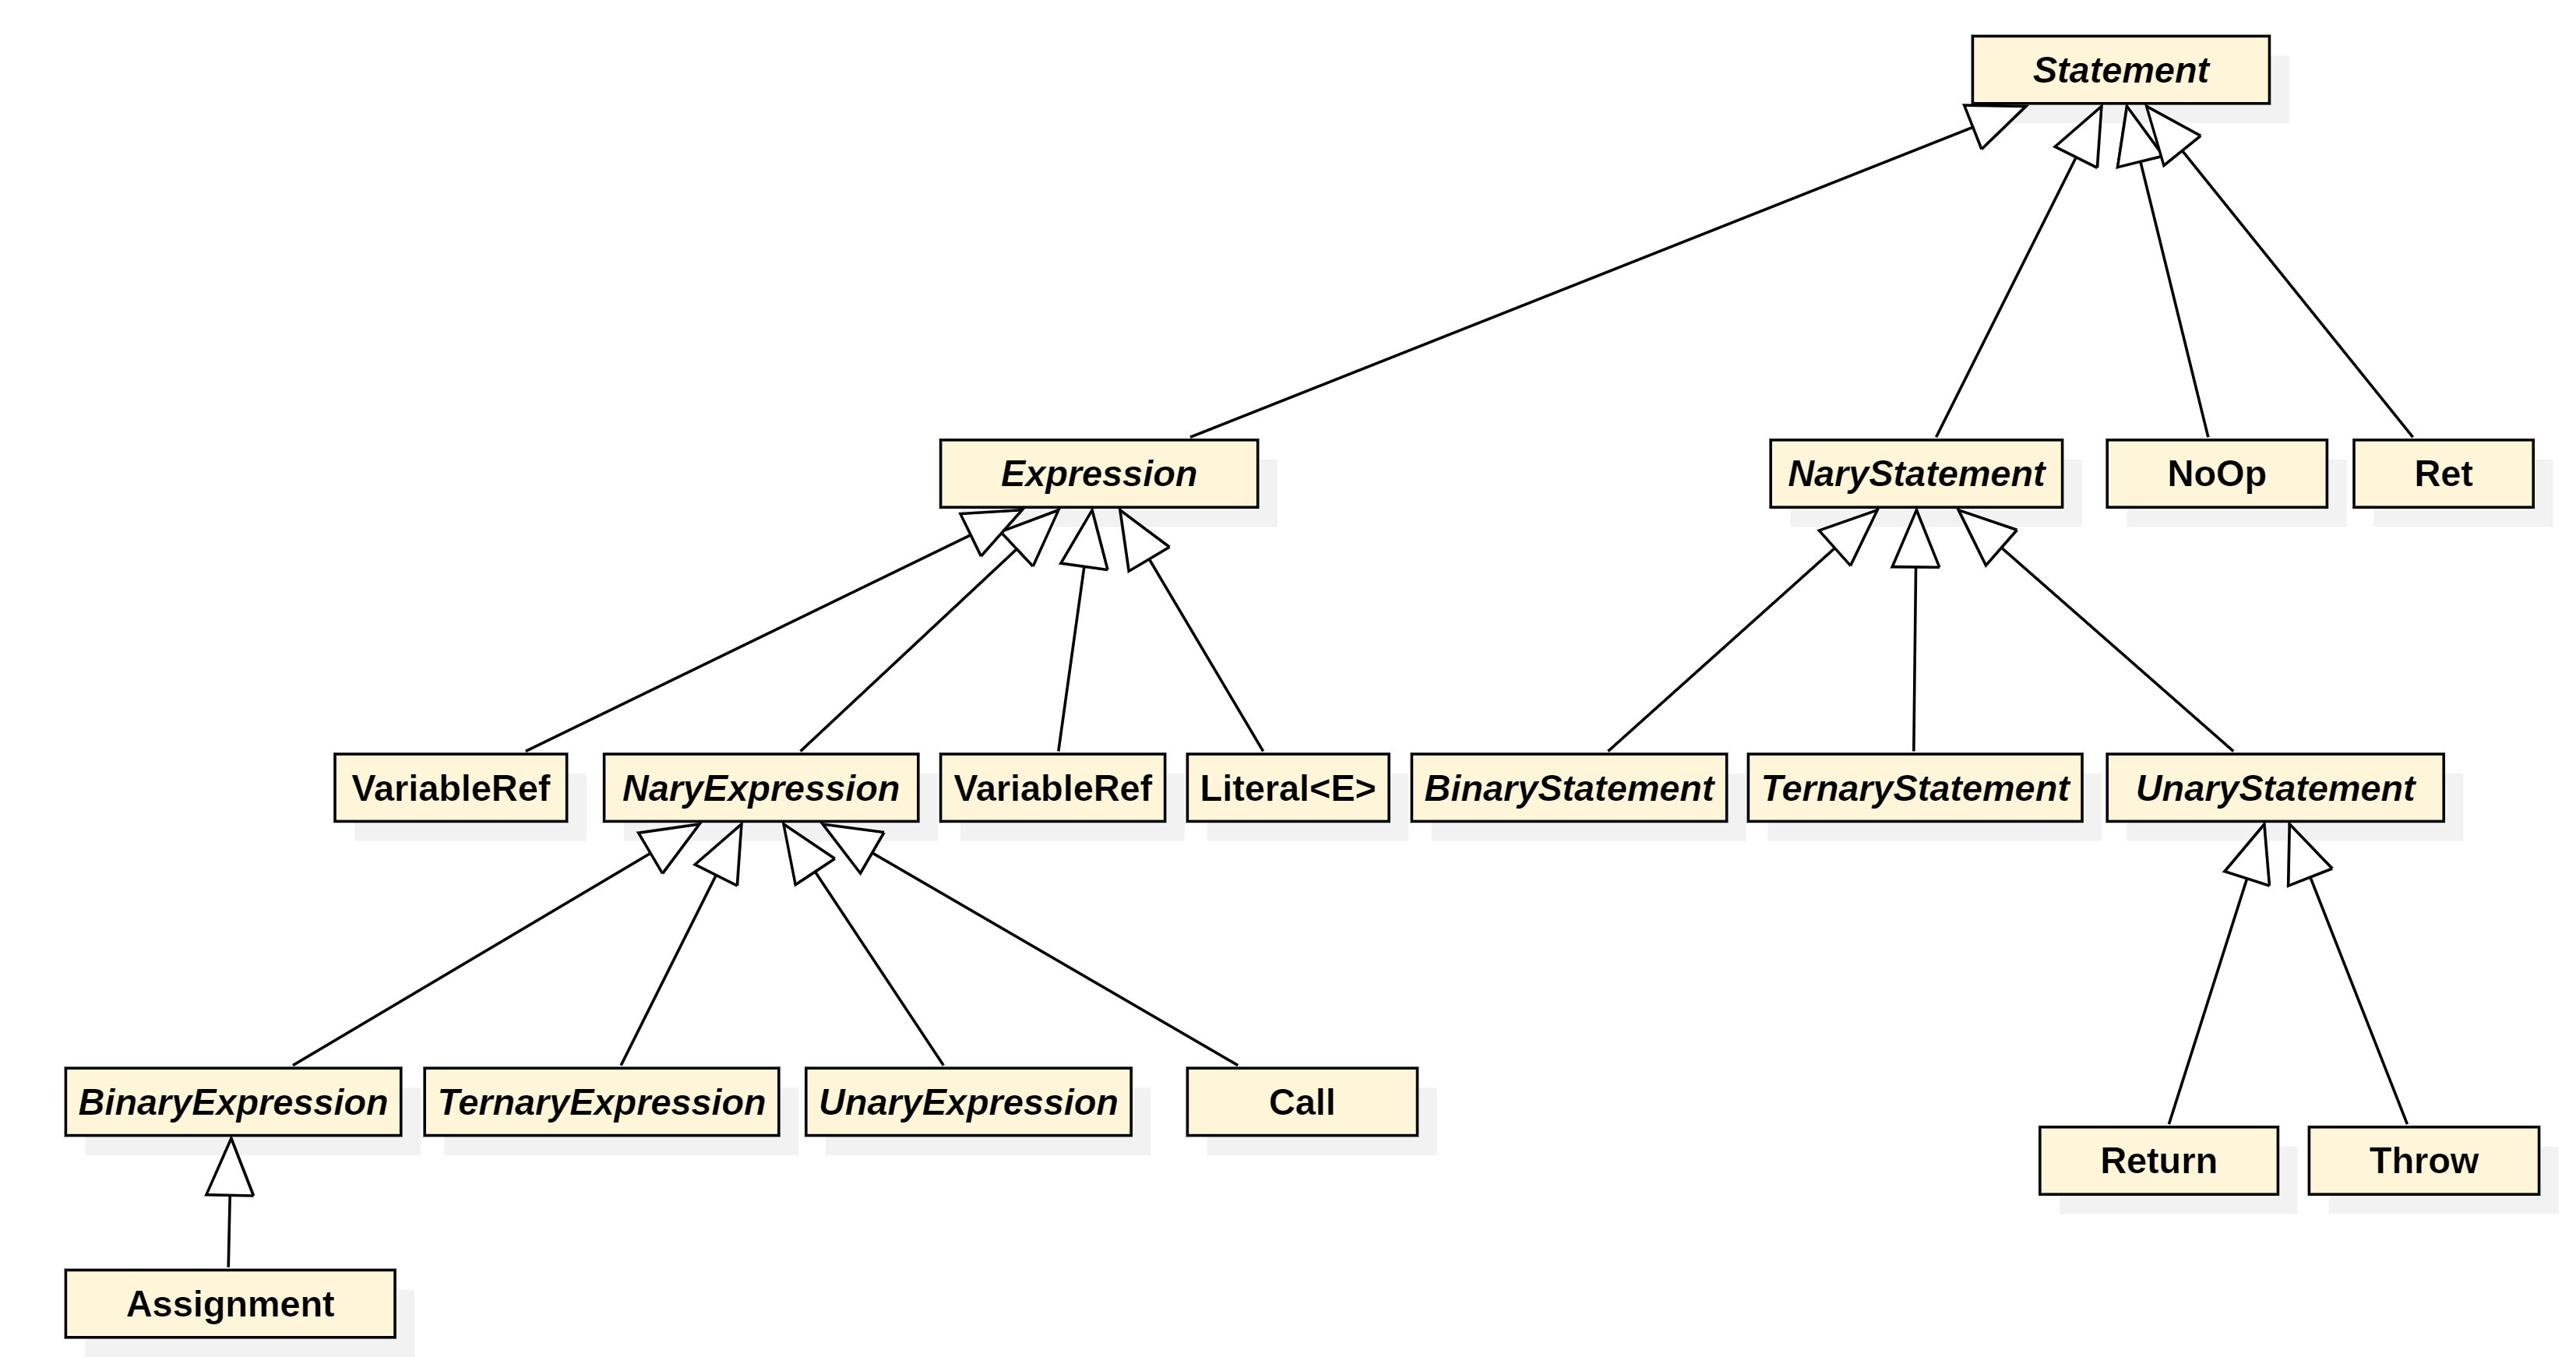
\includegraphics[width=0.9\textwidth]{Immagini/gerarchiaStatement.png}
	\caption{Gerarchia della classe \texttt{Statement}.}
	\label{fig:gerarchiaStatement}
\end{figure}

\subsubsection{\texttt{Edge}}
La classe \texttt{Edge} collega tra di loro due nodi. Esistono tre tipi di \texttt{Edge}: \texttt{SequentialEdge}, modella un flusso senza condizione e sequenziale dal nodo di origine al nodo target, \texttt{TrueEdge}, modella un flusso condizionale se la condizione nel nodo di origine è vera, \texttt{FalseEdge}, modella un flusso condizionale se la condizione nel nodo di origine è falsa.
\\

\texttt{Edge} e \texttt{Statement} modificano le istanze del dominio astratto attraverso, rispettivamente, i metodi \texttt{traverse}, che agisce sul post-state del nodo di origine e consegna il valore trasformato al pre-state del nodo target, e \texttt{semantics}, che trasforma il pre-state di un nodo nel suo post-state. Più precisamente però non è la classe \texttt{Statement} che modifica il dominio astratto. Ogni oggetto di tipo \texttt{Statement} infatti viene trascritto in una composizione di \texttt{SymbolicExpression} a run-time durante l'analisi. Ogni \texttt{SymbolicExpression} ha un significato semantico ben preciso e le istanze del dominio astratto definiscono gli effetti semantici su quest'ultime e non sugli \texttt{Statement}. Possiamo vedere gli \texttt{Statement} come la sintassi e le \texttt{SymbolicExpression} come la semantica dei CFG in LiSA. Le \texttt{SymbolicExpression} si dividono in due principali tipi di espressione, abbiamo le \texttt{HeapExpression}, ovvero le espressioni che modellano le operazioni sull'heap (come \texttt{HeapAllocation}, \texttt{AccessChild}), e le \texttt{ValueExpression}, che modellano modifiche e operazioni sul valore di variabili e costanti (qui per esempio abbiamo \texttt{Addition}, \texttt{LessOrEqual}, \texttt{And}, \texttt{Modulo}, etc..). In figura \ref{fig:gerarchiaSymbolic} qua sotto si vede la non completa gerarchia delle \texttt{SymbolicExpression}.

\begin{figure}[ht]
	\centering
	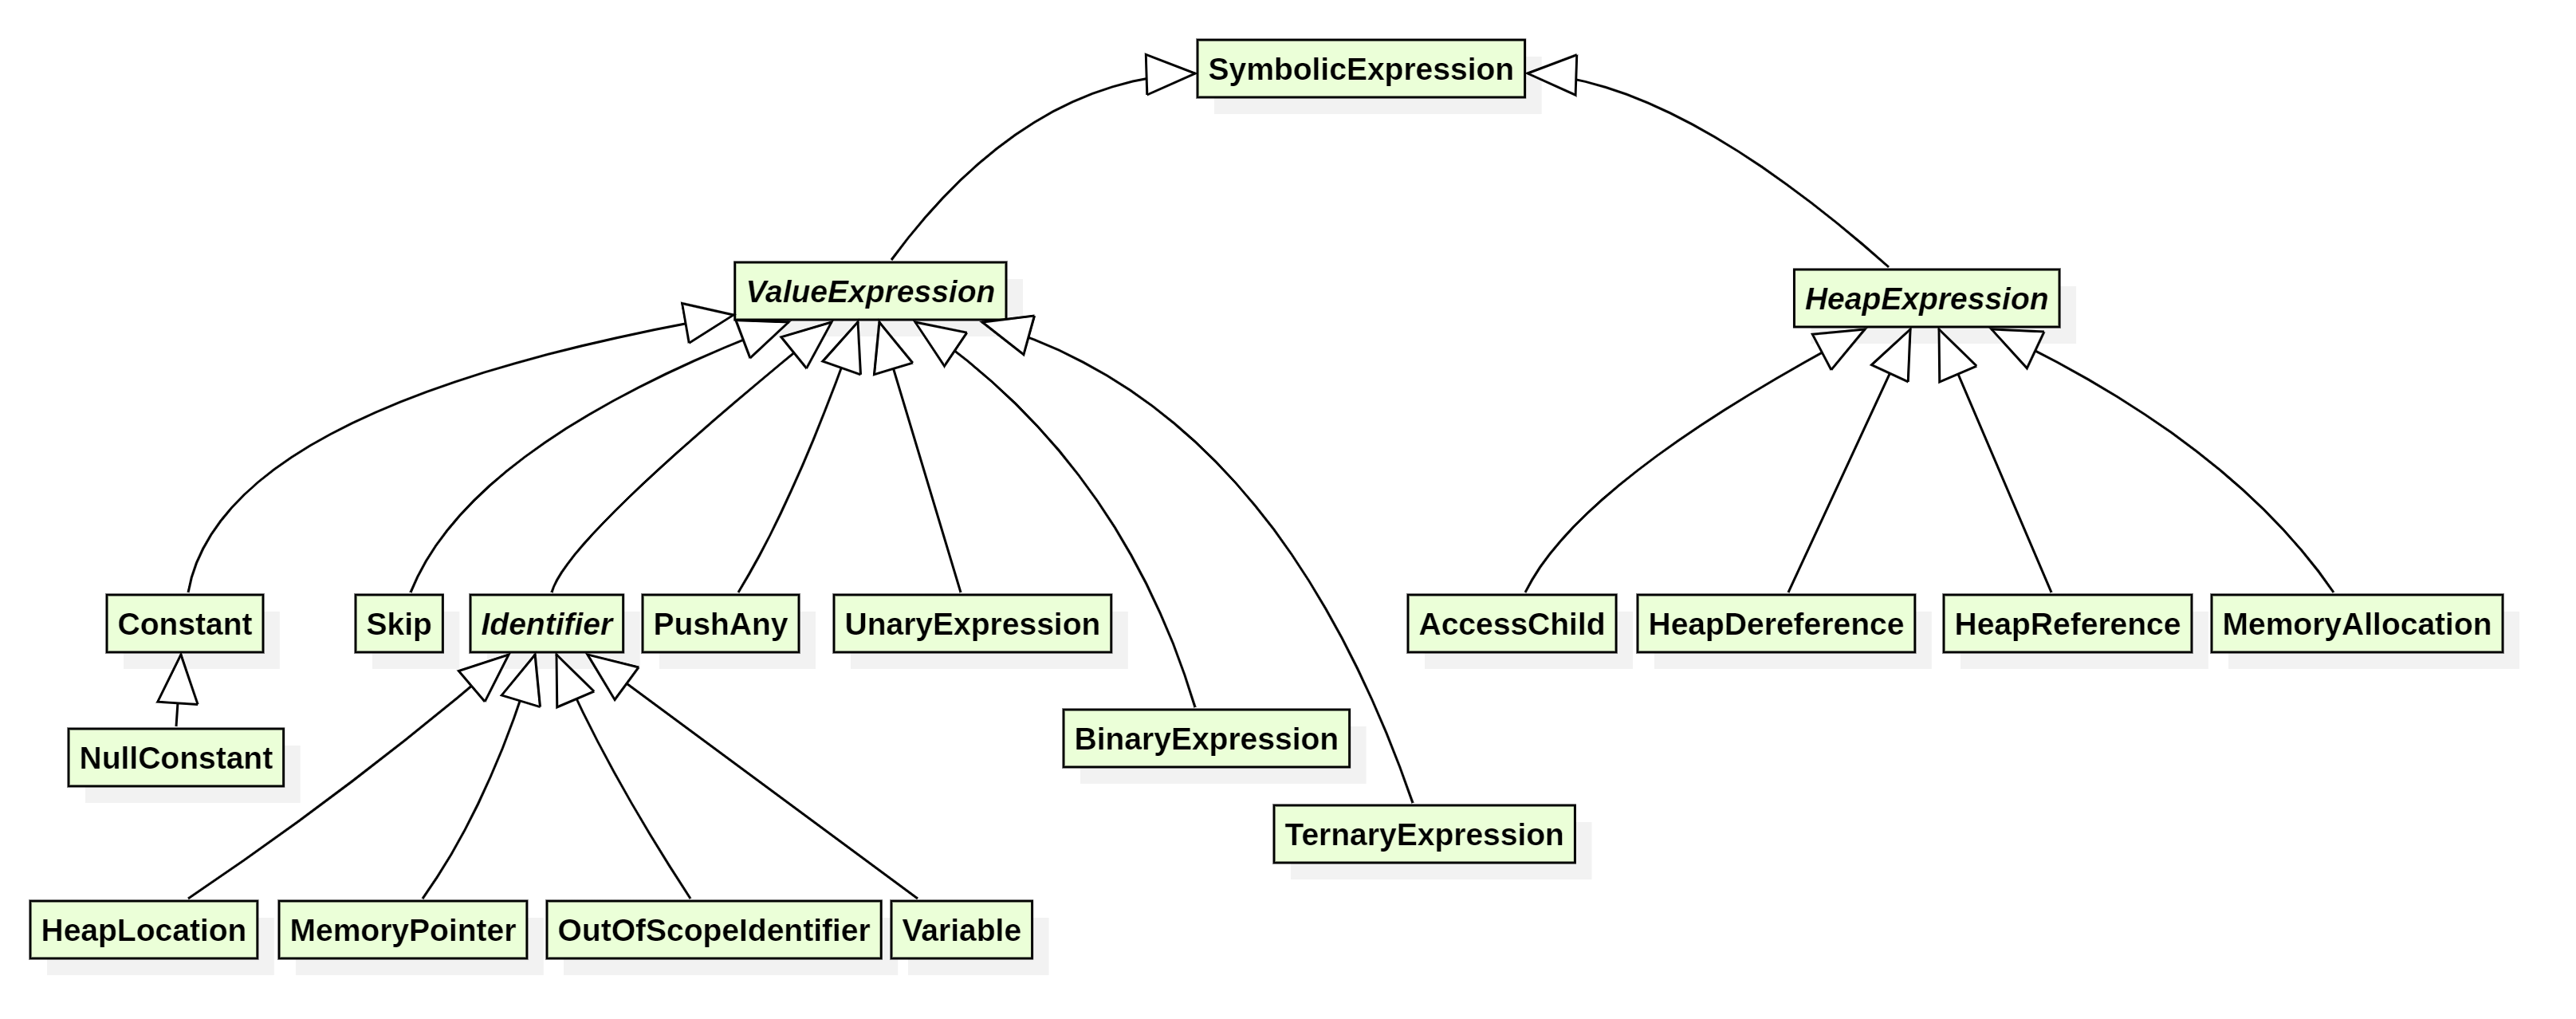
\includegraphics[width=0.9\textwidth]{Immagini/gerarchiaSymbolicExpression.png}
	\caption{Gerarchia della classe \texttt{SymbolicExpression}.}
	\label{fig:gerarchiaSymbolic}
\end{figure}


Per fare un esempio prendiamo in considerazione lo statement \texttt{x = a + b} in un linguaggio non tipato (come Python), in cui non sappiamo i tipi dei valori di \texttt{a} e \texttt{b}. Questo statement in LiSA può essere tradotto in due espressioni simboliche, una per le parte sinistra, ovvero un riferimento alla variabile \texttt{x}, che può essere ulteriormente processata dal dominio astratto che modula l'heap, e una per la parte destra e modella la semantica dell'addizione \texttt{a + b}. Questa può anche controllare i tipi delle due variabili a run-time e in alcuni casi generare una \texttt{SymbolicExpression} che rappresenta l'addizione tra interi (se le due variabili possono avere valori numerici interi) e in altri casi una che rappresenta la concatenazione di stringhe (se entrambe possono contenere stringhe), o qualsiasi altro tipo di operazione modellata tramite il \texttt{+} che dipende dalle caratteristiche dei suoi operandi.
Questa traduzione run-time degli \texttt{Statement} in più \texttt{SymbolicExpression} rende i CFG di LiSA dinamici e plastici, quindi capaci di rappresentare un grande numero di costrutti semantici e la possibilità di modellare le funzioni della maggior parte dei linguaggi. Il compito del front-end in LiSA sarà quello di trasformare un programma scritto in un qualsiasi linguaggio di programmazione in un insieme di CFG comprendibili a LiSA, fatti di \texttt{Statement} (anche language-specific) e \texttt{edge}, e capaci di simulare \textit{completamente} la semantica del programma originale.

\subsection{Domini astratti in LiSA}\label{sec:abstractDomainLiSA}
Ora parleremo invece di come sono definiti in LiSA i domini astratti. Ogni dominio in LiSA implementa due interfacce: \texttt{SemanticDomain}, che rende il dominio capace di valutare l'esecuzione di \texttt{SymbolicExpression} su istanze di esso, e \texttt{Lattice}, che fornisce al dominio le caratteristiche di un reticolo. Ora vediamo queste due interfacce più nel dettaglio.

\subsubsection{\texttt{SemanticDomain}}\label{subsec:semanticDomain}
L'interfaccia \texttt{SemanticDomain<D, E, I>} è parametrica all'istanza concreta D, agli \texttt{Identifier} I e alle \texttt{SymbolicExpression} E. Rappresenta un dominio che è capace di ragionare sulla semantica delle \texttt{SymbolicExpression} di tipo E su \texttt{Identifier} di tipo I. Un dominio semantico D deve implementare i seguenti metodi:
\begin{itemize}
\setlength\itemsep{0.1em}
    \item \texttt{D assign(I id, E exp)}: restituisce un istanza del dominio in cui viene assegnato il valore di \texttt{exp} ad \texttt{id};
    \item \texttt{D assume(E exp)}: restituisce una istanza del dominio in cui si assume che \texttt{exp} sia vera;
    \item \texttt{D forgetIdentifier(I id)}: restituisce una istanza del dominio in cui viene scordata qualsiasi informazione riguardante l'identificatore \texttt{id};
    \item \texttt{D forgetIdentifiers(Collection<I> ids)}: restituisce una istanza del dominio in cui viene scordata qualsiasi informazione riguardante gli identificatori \texttt{ids};
    \item \texttt{Satisfiability satisfies(E exp)}: restituisce un valore (tra \texttt{SATISFIED}, \texttt{UNKNOWN}, \texttt{NOT\_SATISFIED} e \texttt{BOTTOM}) che indica se la espressione \texttt{exp} è soddisfatta nell'istanza del dominio su cui viene chiamata;
    \item \texttt{D smallStepSemantics(E exp)}: restituisce una istanza del dominio modificata dagli effetti della espressione \texttt{exp};
\end{itemize}

\subsubsection{\texttt{Lattice}}\label{subsec:lattice}
L'interfaccia \texttt{Lattice<L>} è parametrica all'istanza concreta L. Un reticolo in LiSA deve implementare questi metodi:
\begin{itemize}
\setlength\itemsep{0.1em}
    \item \texttt{boolean lessOrEqual(L other)}: questo metodo definisce l'ordine parziale del reticolo e restituisce \texttt{true} se l'oggetto su cui viene chiamato è in relazione con \texttt{other};
    \item \texttt{L lub(L other)}: definisce l'operazione di least upper bound e restituisce il lub tra questo oggetto e \texttt{other};
    \item \texttt{L glb(L other)}: definisce l'operazione di greatest lower bound e restituisce il glb tra questo oggetto e \texttt{other};
    \item \texttt{L top(L other)}: restituisce l'elemento \(\top\) del reticolo;
    \item \texttt{L bottom(L other)}: restituisce l'elemento \(\perp\) del reticolo;
    \item \texttt{L widening(L other)}: definisce l'operazione di widening del reticolo e restituisce il widening tra questo oggetto e \texttt{other};
    \item \texttt{L narrowing(L other)}: definisce l'operazione di narrowing del reticolo e restituisce il narrowing tra questo oggetto e \texttt{other} (di defualt il narrowing esegue il glb);
    \item \texttt{boolean isTop()}: restituisce \texttt{true} se l'istanza su cui viene chiamata è l'elemento \(\top\);
    \item \texttt{boolean isBottom()}: restituisce \texttt{true} se l'istanza su cui viene chiamata è l'elemento \(\perp\);
\end{itemize}
In LiSA sono definite alcune implementazioni base di reticoli con comportamenti simili. Innanzitutto è definita l'interfaccia \texttt{BaseLattice} che estende \texttt{Lattice}, la quale definisce i casi base comuni a tutti i reticoli (ovvero le relazioni tra gli oggetti e gli elementi \(\top\) e \(\perp\)). A partire da questa sono poi implementate le classi astratte che definiscono il \texttt{SetLattice<E>} e \texttt{InverseSetLattice<E>} visti nell'esempio \ref{ex:setLattice} e il \texttt{FunctionalLattice<K,E>}, parametrico al tipo K del dominio della funzione e al tipo E del codominio nonchè dominio di un reticolo, visto nell'esempio \ref{ex:functionalLattice}. 


\subsubsection{Lo stato dell'analisi in LiSA: \texttt{AnalysisState}}

Vediamo ora come LiSA organizza lo stato dell'analisi. Lo stato dell'analisi è l'oggetto che viene mappato ad ogni nodo del CFG e indica l'astrazione della semantica  concreta che si vuole approssimare in quel punto di programma (solitamente in LiSA è una astrazione della collecting semantics, ovvero la semantica che ci dice tutti i possibili valori della memoria in un dato punto di programma o equivalentemente l'insieme di tutti gli stati attraversabili durante l'esecuzione del programma). Lo stato dell'analisi è costruito modularmente bottom-up come mostrato in figura \ref{fig:analysisState}.

\begin{figure}
\centering
\tikzset{every picture/.style={line width=0.75pt}} %set default line width to 0.75pt  
\begin{tikzpicture}[x=0.75pt,y=0.75pt,yscale=-1,xscale=1]
%uncomment if require: \path (0,300); %set diagram left start at 0, and has height of 300

%Rounded Rect [id:dp5259274252543102] 
\draw  [fill={rgb, 255:red, 245; green, 236; blue, 218 }  ,fill opacity=1 ][general shadow={fill={rgb, 255:red, 0; green, 0; blue, 0 }  ,shadow xshift=3.75pt,shadow yshift=-3.75pt, opacity=0.15 }] (20.67,194.89) .. controls (20.67,205.94) and (29.62,214.89) .. (40.67,214.89) -- (100.67,214.89) .. controls (111.71,214.89) and (120.67,205.94) .. (120.67,194.89) -- (120.67,72.59) .. controls (120.67,61.55) and (111.71,52.59) .. (100.67,52.59) -- (40.67,52.59) .. controls (29.62,52.59) and (20.67,61.55) .. (20.67,72.59) -- cycle ;
%Rounded Rect [id:dp40217338693406735] 
\draw  [fill={rgb, 255:red, 250; green, 225; blue, 225 }  ,fill opacity=1 ][general shadow={fill={rgb, 255:red, 0; green, 0; blue, 0 }  ,shadow xshift=1.5pt,shadow yshift=-1.5pt, opacity=0.15 }] (28.17,166.69) .. controls (28.17,176.08) and (35.78,183.69) .. (45.17,183.69) -- (96.17,183.69) .. controls (105.56,183.69) and (113.17,176.08) .. (113.17,166.69) -- (113.17,97.64) .. controls (113.17,88.25) and (105.56,80.64) .. (96.17,80.64) -- (45.17,80.64) .. controls (35.78,80.64) and (28.17,88.25) .. (28.17,97.64) -- cycle ;
%Shape: Rectangle [id:dp7147766556498871] 
\draw  [fill={rgb, 255:red, 249; green, 233; blue, 254 }  ,fill opacity=1 ][general shadow={fill={rgb, 255:red, 0; green, 0; blue, 0 }  ,shadow xshift=0.75pt,shadow yshift=-0.75pt, opacity=0.15 }] (35,159.14) .. controls (35,157.49) and (36.34,156.14) .. (38,156.14) -- (102,156.14) .. controls (103.66,156.14) and (105,157.49) .. (105,159.14) -- (105,171) .. controls (105,172.66) and (103.66,174) .. (102,174) -- (38,174) .. controls (36.34,174) and (35,172.66) .. (35,171) -- cycle ;
%Shape: Rectangle [id:dp6945641114766774] 
\draw  [color={rgb, 255:red, 0; green, 0; blue, 0 }  ,draw opacity=1 ][fill={rgb, 255:red, 229; green, 240; blue, 250 }  ,fill opacity=1 ][general shadow={fill={rgb, 255:red, 0; green, 0; blue, 0 }  ,shadow xshift=0.75pt,shadow yshift=-0.75pt, opacity=0.15 }] (35,136.14) .. controls (35,134.49) and (36.34,133.14) .. (38,133.14) -- (102,133.14) .. controls (103.66,133.14) and (105,134.49) .. (105,136.14) -- (105,148) .. controls (105,149.66) and (103.66,151) .. (102,151) -- (38,151) .. controls (36.34,151) and (35,149.66) .. (35,148) -- cycle ;
%Shape: Rectangle [id:dp6352913495307582] 
\draw  [fill={rgb, 255:red, 234; green, 247; blue, 230 }  ,fill opacity=1 ][general shadow={fill={rgb, 255:red, 0; green, 0; blue, 0 }  ,shadow xshift=0.75pt,shadow yshift=-0.75pt, opacity=0.15 }] (35,113.14) .. controls (35,111.49) and (36.34,110.14) .. (38,110.14) -- (102,110.14) .. controls (103.66,110.14) and (105,111.49) .. (105,113.14) -- (105,125) .. controls (105,126.66) and (103.66,128) .. (102,128) -- (38,128) .. controls (36.34,128) and (35,126.66) .. (35,125) -- cycle ;
%Shape: Rectangle [id:dp47123715282050216] 
\draw  [fill={rgb, 255:red, 233; green, 244; blue, 242 }  ,fill opacity=1 ][general shadow={fill={rgb, 255:red, 0; green, 0; blue, 0 }  ,shadow xshift=0.75pt,shadow yshift=-0.75pt, opacity=0.15 }] (35,193.14) .. controls (35,191.49) and (36.34,190.14) .. (38,190.14) -- (102,190.14) .. controls (103.66,190.14) and (105,191.49) .. (105,193.14) -- (105,205) .. controls (105,206.66) and (103.66,208) .. (102,208) -- (38,208) .. controls (36.34,208) and (35,206.66) .. (35,205) -- cycle ;


% Text Node
\draw (31,61) node [anchor=north west][inner sep=0.75pt]  [font=\footnotesize] [align=left] {AnalysisState};
% Text Node
\draw (33,90) node [anchor=north west][inner sep=0.75pt]  [font=\footnotesize] [align=left] {AbstractState};
% Text Node
\draw (39.2,113.2) node [anchor=north west][inner sep=0.75pt]   [align=left] {{\scriptsize \texttt{HeapDomain}}};
% Text Node
\draw (37.2,136.2) node [anchor=north west][inner sep=0.75pt]   [align=left] {{\scriptsize \texttt{ValueDomain}}};
% Text Node
\draw (40.6,159.8) node [anchor=north west][inner sep=0.75pt]   [align=left] {{\scriptsize \texttt{TypeDomain}}};
% Text Node
\draw (45.4,193.4) node [anchor=north west][inner sep=0.75pt]   [align=left] {{\scriptsize Expr stack}};
\end{tikzpicture}
    \caption{Architettura dello stato dell'analisi in LiSA.}
    \label{fig:analysisState}
\end{figure}

La classe che definisce lo stato dell'analisi è \texttt{AnalysisState}. \'E formato da due componenti: un \texttt{AbstractState} e lo stack delle espressioni, ovvero l'insieme di \texttt{SymbolicExpression} che rimangono sullo stack dopo il calcolo di una espressione (è importante notare che questa è solo una visione sommaria dell'\texttt{AnalysisState}). Il principale compito di questa classe è quello però di fare da wrap tra l'\texttt{AbstractState} e informazioni semantiche aggiuntive utili al raggiungimento del fix-point durante il calcolo dell'analisi. L'\texttt{AnalysisState} implementa entrambe le interfacce mostrate prima (\hyperref[subsec:lattice]{\texttt{Lattice}} e \hyperref[subsec:semanticDomain]{\texttt{SemanticDomain}}) rendendolo un oggetto sia capace di ragionare sulla semantica delle espressioni simboliche che un sistema ordinato con le caratteristiche di un reticolo. Ogni sua componente, scendendo gerarchicamente nella struttura, implementa queste due interfacce. L'\texttt{AbstractState} è l'astrazione dello stato della memoria e, come si vede dall'immagine, è composto da tre sotto-domini (ognuno dei quali implementa le interfacce \hyperref[subsec:lattice]{\texttt{Lattice}} e \hyperref[subsec:semanticDomain]{\texttt{SemanticDomain}}): 
\begin{itemize}
\setlength\itemsep{0.1em}
    \item un \texttt{HeapDomain} che è responsabile di tracciare l'evoluzione dello stato della memoria dinamica durante l'esecuzione. Opera prima del \texttt{ValueDomain} e risolve gli indirizzi traducendo le espressioni simboliche e rinominando le variabili in modo tale che il \texttt{ValueDomain} possa comprenderle e si preocccupi \textit{solamente} di tracciarne le proprietà;
    
    \item un \texttt{ValueDomain} che è responsabile di tracciare proprietà astratte (come per esempio il valore astratto) delle variabili (possibilmente pre-processate e riscritte prima dall'\texttt{HeapDomain}) del programma. In LiSA è possibile definire \texttt{ValueDomain} sia relazionali (come i Polyhedra) sia non. Per quest'ultimi è definita dentro LiSA una classe base chiamata \texttt{Environment} che estende  \texttt{FunctionalLattice<Identifier, L>} ed implementa \texttt{SemanticDomain}, capace di tracciare un valore del dominio astratto \texttt{L} (che può essere per esempio un Interval, un Sign, un Modulo) ad ogni identificatore tenuto in memoria. Va sottolineato che il dominio \texttt{L} di un \texttt{Environment} ha si la struttura reticolare, ed estende \texttt{Lattice}, e può anche ragionare semanticamente sulle \texttt{SymbolicExpression} senza però implementare \texttt{SemanticDomain}. Infatti per il caso specifico dei domini non-relazionali gestiti tramite \texttt{Environment} il dominio astratto si costruirà attraverso l'interfaccia \texttt{NonRelationalDomain} che ha solo un sottoinsieme dei metodi di \texttt{SemanticDomain}. Per capire perchè pensiamo ai metodi \texttt{assign}, \texttt{forgetIdentifier/s} in \texttt{SemanticDomain}. La definizione di questi metodi, potenzialmente, è uguale per tutti i domini non-relazionali, ed infatti di queste se ne prende carico la classe \texttt{Environment}, lasciando alla creazione dei domini astratti non-relazionali solo la necessità di definire: (i) le operazioni riguardanti la struttura reticolare del dominio (lub, glb, lessOrEqual, \(\cdots\)), e (ii) la logica per la valutazione delle espressioni simboliche;
    
    \item un \texttt{TypeDomain} che è un \texttt{ValueDomain} non-relazionale (quindi costruito a partire da \texttt{Environment}) che associa ad ogni variabile l'insieme dei possibili tipi a run-time delle variabili. Questa può essere usata durante l'analisi per generare espressioni simboliche specifiche a seconda dei tipi delle variabili coinvolte nello statement;
\end{itemize}

L'\texttt{AbstractState} principalmente fa quindi da coordinatore tra l'\texttt{HeapDomain} e il \texttt{ValueDoamin}, passando all'ultimo le espressioni tradotte e gli identificatori trasformati dal primo quando i due mondi devono comunicare e invece compartizzando e separando i due domini quando le espressioni riguardano solo uno dei due.

\subsection{Calcolo del fix-point in LiSA}\label{sec:fix-pointLiSA}
Abbiamo visto nella sezione \ref{sec:abstractInt} che fare interpretazione astratta non significa altro che trovare una soluzione ad un sistema di equazioni costruito a partire dal CFG del programma. Tutte le soluzioni del sistema sono per definizione suoi fix-point e quindi cercare la soluzione significa cercarne un fix-point (possibilmente il più preciso, ovvero il least fix-point). Come viene mostrato nell'introduzione dell'articolo di Cousot \cite{Cousot-IMAG-RR88-1977} qualsiasi metodo caotico di risoluzione ci permette di ottenere una soluzione del sistema (non necessariamente la minima). Tra tutti questi metodi ci conviene usarne uno efficiente e che sfrutti la struttura del CFG in modo da velocizzare la convergenza verso un fix-point. L'algoritmo che viene utilizzato in LiSA per la risoluzione del sistema di equazioni è quello classico basato su working-set e prima dell'implementazione della fase discendente seguiva la definizione in pseudo-codice fornita in \ref{alg:fixpointAsc}.

\begin{algorithm}
	\caption{Algoritmo per il calcolo del fix-point con working-set list con solo fase ascendente.}
	\label{alg:fixpointAsc}
	\begin{algorithmic}[1]
		\Statex
		%\Function{MST-Prim}{grafo G, funzione\_peso $\omega$, nodo\_radice r}\\
        
		\Let{\textit{result}}{\{\}}
        \Let{\textit{ws}}{\(\{st_0\}\)}
        \While{\(ws\neq \emptyset\)}
            \Let{\textit{st}}{\(pop(ws)\)}
            \Let{\(in_{st}\)}{\(\bigsqcup\{traverse_{prev\rightarrow st}(out_{prev})\ |\ prev \in preds(st)\}\)}
            \Let{\(out_{st}\)}{\(semantics_{st}(in_{st})\)}
            \If{\textbf{not }\(out_{st} \leq result[st]\)}
                \If{il widening threshold è stato raggiunto}
                    \Let{\(result[st]\)}{\(result[st]\nabla out_{st}\)}
                \Else
                    \Let{\(result[st]\)}{\(result[st]\sqcup out_{st}\)}
                \EndIf
                \Let{\(ws\)}{\(ws\cup succs(st)\)}
            \EndIf
        \EndWhile
		\State \Return{\textit{result}}
        
		%\EndFunction
	\end{algorithmic}
\end{algorithm}

\iffalse
\begin{algorithm}
	\caption{Algoritmo per il calcolo del fix-point con working-set list con solo fase ascendente.}
	\label{alg:prova}
	\begin{algorithmic}[1]
		\Statex
		%\Function{MST-Prim}{grafo G, funzione\_peso $\omega$, nodo\_radice r}\\
        
		\Let{\textit{result}}{\{\}}
        \Let{\textit{ws}}{\(\{st_0\}\)}
        \While{\(ws\neq \emptyset\)}
            \Let{\textit{st}}{\(pop(ws)\)}
            \Let{\(in_{st}\)}{\(\bigsqcup\{traverse_{prev\rightarrow st}(out_{prev})\ |\ prev \in preds(st)\}\)}
            \Let{\(out_{st}\)}{\(semantics_{st}(in_{st})\)}
            \If{\textbf{not }\(out_{st} \textcolor{red}{\cong} result[st]\)}
                \If {\textcolor{red}{heuristic()}}
                    \Let{\(result[st]\)}{\(result[st]\textcolor{red}{\otimes} out_{st}\)}
                \Else
                    \Let{\(result[st]\)}{\(result[st]\textcolor{red}{\oplus} out_{st}\)}
                \EndIf
                \Let{\(ws\)}{\(ws\cup succs(st)\)}
            \EndIf
        \EndWhile
		\State \Return{\textit{result}}
        
		%\EndFunction
	\end{algorithmic}
\end{algorithm}
\fi

Nell'algoritmo \(result\) è una mappa che associa ogni statement del grafo ad uno stato astratto (in LiSA in sostanza è una istanza di \texttt{Map<Statement, AnalysisState>}). All'inizio la mappa è vuota (che può essere visto come il partire dall'elemento \(\perp\)). \(ws\) è la lista contenente gli statement ancora da calcolare e inizialmente viene caricata con l'entry-point del CFG (ovvero \(st_0\)). Si entra poi in un ciclo while che viene ripetuto finchè nella \(ws\) sono presenti statement. I passaggi all'interno del while sono:
\begin{enumerate}
\itemsep0em 
    \item si estrae un elemento dal \(ws\);
    \item viene calcolato il pre-state dello statement facendo il lub tra tutti i post-state degli statement precedenti al corrente, applicando ad essi la funzione semantica propria dell'arco che connette i due nodi (in LiSA questa sarebbe il metodo \texttt{traverse} delle istanze della classe \texttt{Edge});
    \item si calcola il post-state dello statement facendo passare il pre-state attraverso la funzione semantica propria del nodo corrente (in LiSA questa è il metodo \texttt{semantics} delle istanze della classe \texttt{Statement}).
    \item si controlla se il post-state del nodo sia minore o uguale allo stato astratto mappato a quello statement in \(result\). Se ciò che abbiamo calcolato nel post-state è minore od uguale a quello che abbiamo già possiamo evitare di aggiungere i nodi successivi al corrente in \(ws\), perchè siamo sicuri di non poter dare loro nessuna informazione in più che già non gli abbiamo dato precedentemente e che quindi non li aiuterebbe a cambiare il loro post-state. Se invece non è minore o uguale bisogna aggiornare \(result\) e propagare il cambiamento a tutti gli statement successivi a quello corrente sotto analisi. 
    \item se siamo entrati nel corpo dell'if a riga 7 vuol dire che dobbiamo aggiornare \(result\). Come abbiamo visto nel capitolo sull'intepretazione astatta per raggiungere un fix-point (che sia il least fix-point o una approssimazione di esso) dobbiamo applicare un'operazione di join tra i risultati degli step della iterazione sul sistema di equazioni. Questa operazione di join deve essere un operatore di upper bound (quindi il lub o una sua approssimazione, per esempio il widening). Per scegliere se usare il widening o il lub settiamo a priori nell'analisi un valore di threshold. Una volta passati threshold volte per uno statement durante l'analisi passiamo dall'usare il lub all'usare il widening. Questa logica decisionale ci permette di garantire la finitudine dell'analisi, infatti siamo sicuri che dopo un numero finito di step si cominci ad usare il widening, il quale a sua volta, come abbiamo visto, ci garantisce la convergenza. Infine, dopo aver aggiornato \(result\), dobbiamo garantire di propagare i cambiamenti effettuati e quindi inseriamo tutti gli statement successivi al corrente nel \(ws\). 
\end{enumerate}
Prima o poi non ci sono più aggiornamenti da fare a \(result\) e quindi non vengono più aggiunti statement a \(ws\), che di conseguenza si svuota e rende falsa la condizione del ciclo while alla riga 3 terminando la computazione e lasciando in \(result\) un fix-point, e quindi una soluzione, del sistema di equazioni generato a partire dal CFG.
\iffalse
\\

Dove:
\begin{itemize}
\itemsep0pt
    \item \textcolor{red}{\(\cong\)} è \(\preceq\) nella fase ascendente \\ e \(\succeq\) nella fase discendente;
    \item \textcolor{red}{\(\otimes\)} è \(\nabla\) nella fase ascendente \\ e \(\Delta\) nella fase discendente;
    \item \textcolor{red}{\(\oplus\)} è \(\sqcup\) nella fase ascendente \\ e \(\sqcap\) nella fase discendente;
    \item \textcolor{red}{heuristic()} è une metodo decisionale \\ che ci permette di scegliere se usare \\ \(\sqcup\) (o \(\sqcap\)) o \(\nabla\) (o \(\Delta\));
\end{itemize}
\fi
\definecolor{keywordsColor}{rgb}{0.5, 0.0, 0.333}
\lstset
    {
    basicstyle=\footnotesize\ttfamily,
    breaklines=true,
    keywordstyle=\color{keywordsColor}\bfseries,
    language=Java, 
    numbers=none,
    %showspaces=true,
    literate={\ \ }{{\ }}1,
    frame=single,
    breaklines=true
    }

\subsection{Come fare una semplice analisi in LiSA}
In questa piccola sezione vedremo come utilizzare effettivamente LiSA. Il frammento di codice qui di seguito ci permette di analizzare il programma presente in \texttt{programFilePath} utilizzando il \texttt{Frontend} appropriato per il linguaggio in cui è scritto. 
\label{code:simpleAnalysisAsc}
\begin{lstlisting}[belowskip=-1.1 \baselineskip]
LiSAConfiguration conf = new LiSAConfiguration();
conf.abstractState = LiSAFactory.getDefaultFor(
				AbstractState.class, 
				getDefaultFor(HeapDomain.class), 
				new Interval(),
				new TypeEnvironment<>(new InferredTypes()));
conf.wideningThreshold = 5;
conf.analysisGraphs = GraphType.DOT;
conf.workdir = outputDirectory;
Program program = Frontend.processFile(programFilePath);
LiSA lisa = new LiSA(configuration);
lisa.run(program);
\end{lstlisting}
Bisogna innanzitutto configurare l'analisi attraverso un oggetto della classe \texttt{LiSAConfiguration}. Un parametro obbligatorio è lo stato astratto da utilizzare e le sue componenti. In questo caso viene utilizzato quello di default per l'\texttt{HeapDomain}, il dominio non-relazionale \texttt{Interval}, che verrà racchiuso in un \texttt{ValueEnvironment}, per il \texttt{ValueDomain} e il dominio con tipi dedotti per il \texttt{TypeDomain}. Viene poi impostato il tipo di output con cui vogliamo visualizzare i risultati e la cartella in cui vogliamo che venga messo l'output generato dall'analisi. Viene generato il programma (che semplificando può essere visto come una collezione di CFG) tramite il \texttt{Frontend}. Infine viene lanciata l'analisi tramite un oggetto   della classe \texttt{LiSA} passando configurazioni e programma da analizzare. In figura \ref{fig:risultatoDOTAsc} è mostrato l'output generato in DOT con queste configurazioni per il programma mostrato in \ref{fig:codiceEsempio2}.
\begin{figure}[ht]
	\centering
	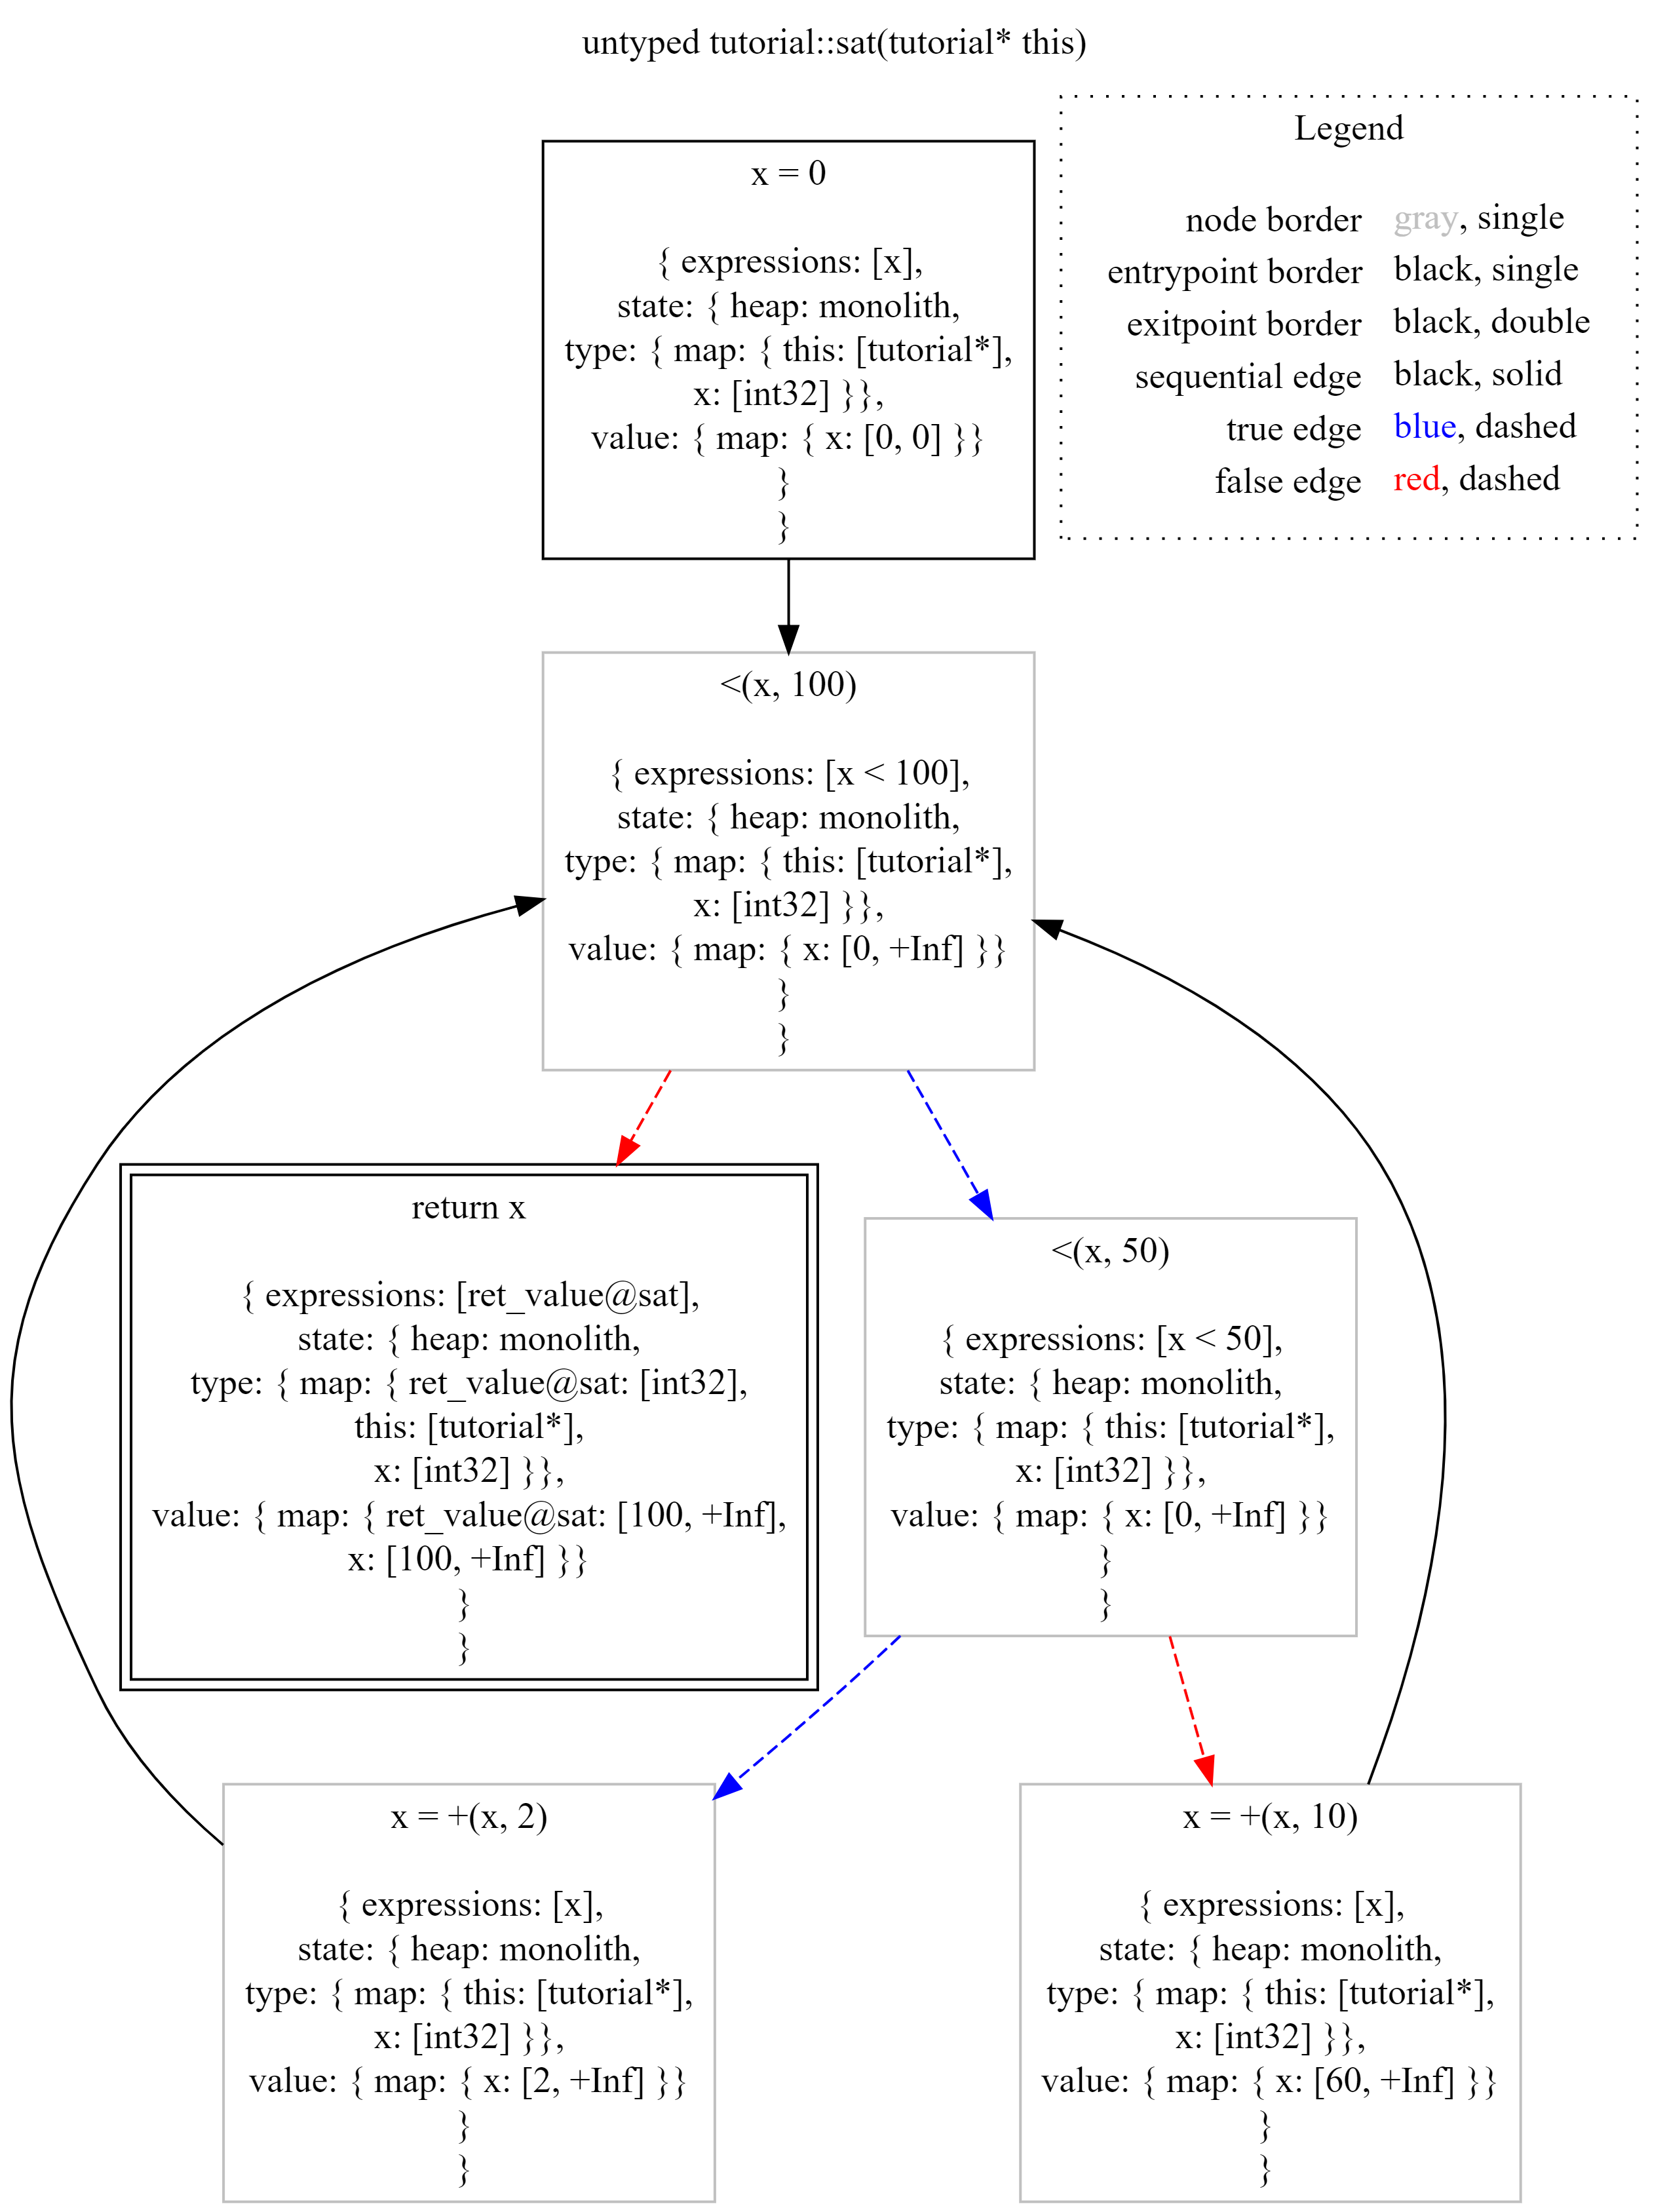
\includegraphics[width=0.8\textwidth]{Immagini/graphviz.png}
	\caption{Risultato in formato DOT dell'analisi con solo fase ascendente del codice nella Figura \ref{fig:codiceEsempio2}.}
	\label{fig:risultatoDOTAsc}
\end{figure}
\\

Fino'ora abbiamo introdotto tutte le nozioni matematiche e teoriche necessarie per capire come funzioni l'analisi statica tramite interpretazione astratta (nel capitolo \hyperref[chapter:background]{Background}) ed abbiamo visto come questi concetti vengono applicati all'interno di LiSA (nella sezione \hyperref[sec:LiSA]{LiSA} di questo capitolo). Da questo punto in poi verrà spiegato il contributo che è stato dato per espandere la libreria, guardando nel dettaglio ogni implementazione. Partiremo dal dominio dei sottoinsiemi non ridondanti di un reticolo, poi passeremo alla fase discendente per poi finire col decoupling delle fasi.

\section{Dominio dell'insieme delle parti finite e non ridondanti in LiSA}

Come abbiamo detto nella piccola introduzione al concetto di \texttt{ValueDomain} in LiSA è possibile sviluppare domini sia relazionali che non. Lo sviluppo nei due casi prende "percorsi" diversi, e questo perchè, abbiamo detto, molte operazioni sono comuni a tutti i domini non-relazionali e quindi aveva senso avere un strato in più che si prendesse carico di queste operazioni comuni, ovvero l'\texttt{Environment}, semplificando all'utente l'operazione di sviluppare domini non-relazionali. Per questo motivo l'introduzione di un sistema generico per lo sviluppo del dominio dell'insieme delle parti finite e non ridondanti di un altro dominio astratto, già definito in LiSA, ha dovuto coprire entrambi casi. Partiamo dal caso generale. 

\subsection{Il caso generale}

Nella Sezione \ref{sec:abstractDomainLiSA} abbiamo mostrato le caratteristiche che deve avere un dominio astratto in LiSA (sottoforma delle interfacce che deve implementare). In \ref{code:nonRedundantPowerset} è mostrata la definizione (non completa) della classe che implementa la versione più generale del concetto di dominio dei sottinsiemi finiti e non ridondanti di un altro dominio.
%(a partire dalla quale si possono sviluppare sia domini relazionali che non).
\begin{algorithm}
\lstset{frame=none}
\begin{lstlisting}[belowskip=-1.1 \baselineskip]
public abstract class NonRedundantPowerset<
        C extends NonRedundantPowerset<C, T, E, I>,
        T extends SemanticDomain<T, E, I> & Lattice<T>,
        E extends SymbolicExpression,
        I extends Identifier> 
    extends SetLattice<C, T> 
    implements SemanticDomain<C, E, I> {

    public final T valueDomain;
    
    public NonRedundantPowerset(Set<T> elements, 
                                boolean isTop, 
                                T valueDomain) {...}
    
    protected C removeRedundancy() {...}
    
    @Override
    public C lubAux(C other) {...}
    
    @Override
    public C glbAux(C other) {...}
    
    protected C EgliMilnerConnector(C other) {...}
    
    protected C extrapolationHeuristic(C other) {...}
    
    @Override
    public C wideningAux(C other) {...}
    
    @Override
    public boolean lessOrEqualAux(C other) {...}
    
    public boolean lessOrEqualEgliMilner(C other) {...}
    
    @Override
    public C mk(Set<T> set) {...}
    
    public abstract C mkAux(Set<T> set, 
                            boolean isTop, 
                            T valueDomain);
    
    @Override
    public Satisfiability satisfies(E expression, 
                                    ProgramPoint pp) {...}
}
\end{lstlisting}
\caption{La classe \texttt{NonRedundantPowerset}.}
\label{code:nonRedundantPowerset}
\end{algorithm}
La classe astratta \texttt{NonRedundantPowerset<C,T,E,I>} è parametrica a quattro classi:
\begin{itemize}
    \itemsep0pt
    \item \texttt{C} è la classe concreta del dominio;
    \item \texttt{T} è il dominio sottostante, ovvero il tipo degli elementi all'interno degli insiemi, e deve avere anche lui le caratteristiche di un dominio astratto (quindi deve implementare le interfacce \texttt{SemanticDomain} e \texttt{Lattice});
    \item \texttt{E} è il tipo delle \texttt{SymbolicExpression} su cui questo dominio, e quindi quello sottostante \texttt{T}, riesce a ragionare semanticamente;
    \item \texttt{I} è il tipo di \texttt{Identifiers} che questo dominio,  e quindi quello sottostante \texttt{T}, sa manipolare;
\end{itemize}\ 
La classe, poi, invece di implementare \texttt{BaseLattice<C>} estende \texttt{SetLattice<C,T>}, che definisce la struttura reticolare che ci serve in questo caso e che viene mostrata formalmente nel capitolo \hyperref[chapter:background]{Background} all'esempio \ref{ex:setLattice}. Sintetizzando molto la classe astratta \texttt{SetLattice} è cosi definita in LiSA:
\begin{lstlisting}[belowskip=-1.1 \baselineskip]
public abstract class SetLattice<S extends SetLattice<S,T>,T> 
    implements BaseLattice<S>, Iterable<T> {

    public final Set<T> elements;
    public boolean isTop;
    ...
}
\end{lstlisting}
Dove \texttt{elements} è l'insieme contenente oggetti di tipo \texttt{T}, il campo \texttt{isTop} traccia il fatto che l'elemento in questioni rappresenti l'elemento top, l'operazione di lub è l'unione tra insiemi \(\cup\) e la relazione di ordine parziale è il contenimento insiemistico \(\subseteq\).

Il campo \texttt{public final T valueDomain} introdotto da \texttt{NonRedundantPowerset} è un elemento qualsiasi del dominio sottostante e serve in alcune operazioni riguardanti la struttura reticolare del dominio per ottenere i valori \texttt{top} e \texttt{bottom}. Il metodo \texttt{public C mk ( Set <T > set )} viene ereditato da \texttt{SetLattice} e serve a costruire una istanza concreta del dominio a partire dagli oggeti contenuti in \texttt{set}. In \texttt{NonRedundantPowerset} è definita in modo tale da richiamare \texttt{mkAux(...)}, ovvero la versione estesa di \texttt{mk} fatta per comprendere \texttt{ValueDomain} e \texttt{isTop}, il quale deve essere definito nelle classi concrete che estendono \texttt{NonRedundantPowerset} (infatti \texttt{mkAux} è dichiarato come metodo astratto).

Un altro metodo molto importante è \texttt{removeRedundancy}. Non è altro che la funzione di riduzione mostrata nella Definizione \ref{def:funzioneRiduzione}. Serve a rimuovere la ridondanza dall'insieme. \'E necessaria perchè alcune operazioni sugli elementi del dominio potrebbero togliergli questa proprietà, che quindi deve essere ripristinata. La definizione del metodo è la seguente:
\begin{lstlisting}[belowskip=-1.1 \baselineskip]
protected C removeRedundancy(){
    Set<T> newElementsSet = new HashSet<T>();
    for (T element : this.elements) {
        if (!element.isBottom()) {
            boolean toRemove = false;
            for (T otherElement : this.elements)
                if (element.lessOrEqual(otherElement) && 
                    !otherElement.lessOrEqual(element))
                    toRemove = true;
            if (!toRemove)
                newElementsSet.add(element);
        }
    }
    return mk(newElementsSet);
}
\end{lstlisting}

\subsubsection{Le operazioni reticolari in \texttt{NonRedundantPowerset}}
Passiamo ora a dare la definizione dei metodi delle operazioni riguardanti la struttura reticolare del dominio. Partiamo dal metodo che definisce l'ordine parziale che segue la Definizione in \ref{def:powersetDomain}.
\begin{lstlisting}[belowskip=-1.1 \baselineskip]
@Override
public boolean lessOrEqualAux(C other) throws SemanticException {
    for (T s1 : this.elements) {
        boolean existsGreaterElement = false;
        for (T s2 : other.elements) {
            if (s1.lessOrEqual(s2)) {
                existsGreaterElement = true;
                break;
            }
        }
        if (!existsGreaterElement)
            return false;
    }
    return true;
}
\end{lstlisting}
Proseguiamo con le operazioni di least upper bound e greatest lower bound che seguono le Definizioni date in \ref{def:powersetDomain}.
\begin{lstlisting}[belowskip=-1.1 \baselineskip]
@Override
public C lubAux(C other) {
    Set<T> lubSet = new HashSet<T>(this.elements);
    lubSet.addAll(other.elements);
    return mk(lubSet).removeRedundancy();
}

@Override
public C glbAux(C other)
        throws SemanticException {
    Set<T> glbSet = new HashSet<T>();
    for (T s1 : this.elements)
        for (T s2 : other.elements)
            glbSet.add(s1.glb(s2));
    return mk(glbSet).removeRedundancy();
}
\end{lstlisting}
Abbiamo poi la relazione di ordine parziale di Egli-Milner che segue la Definizione in \ref{def:EgliMilnerRelation}.
\begin{lstlisting}[belowskip=-1.1 \baselineskip]
public boolean lessOrEqualEgliMilner(C other){
    if (lessOrEqual(other)) {
        if (!isBottom()) {
            for (T s2 : other.elements) {
                boolean existsLowerElement = false;
                for (T s1 : this.elements) {
                    if (s1.lessOrEqual(s2)) {
                        existsLowerElement = true;
                        break;
                    }
                }
                if (!existsLowerElement)
                    return false;
            }
        }
    } else
        return false;
    return true;
}
\end{lstlisting}
Dichiariamo poi un metodo che fa da connettore di Egli-Milner (descritto nella Definizione \ref{def:connettoreEgliMilner}) tra due elementi e ne diamo una implementazione di default, che anche se corretta per ogni dominio è grossolana ed imprecisa (nell'esempio specifico degli \texttt{Interval}, nel caso dei domini non-relazionali, ne vedremo una ridefinizione più "intelligente" che ci permette di preservare precisione nell'analisi).
\begin{lstlisting}[belowskip=-1.1 \baselineskip]
protected C EgliMilnerConnector(C other) {
    Set<T> unionSet = new HashSet<T>(this.elements);
    unionSet.addAll(other.elements);
    T completeLub = valueDomain.bottom();
    if (!unionSet.isEmpty()) {
        for (T element : unionSet) {
            completeLub = completeLub.lub(element);
        }
    }
    Set<T> newSet = new HashSet<T>();
    if (completeLub != null)
        newSet.add(completeLub);
    return mk(newSet);
}
\end{lstlisting}
L'implementazione base semplicemente crea un nuovo insieme singoletto con il least upper bound di tutti gli elementi dei due insiemi uniti. 

\noindent Il widening implementato per i \texttt{NonRedundantPowerset} utilizza un estrapolatore euristico \(\nabla\)-connesso. Per questo seguendo la Definizione \ref{def:estrapolatoreEuristicoWideningConnesso} e la Proposizione \ref{prop:estrapolatoreEuristicoWideningConnesso} lo implementiamo così: 
\begin{lstlisting}[belowskip=-1.1 \baselineskip]
protected C extrapolationHeuristic(C other){
    Set<T> extrapolatedSet = new HashSet<T>();
    for (T s1 : this.elements) {
        for (T s2 : other.elements) {
            if (s1.lessOrEqual(s2) && !s2.lessOrEqual(s1))
                extrapolatedSet.add(s1.widening(s2));
        }
    }
    return mk(extrapolatedSet).removeRedundancy().lub(other);
}
\end{lstlisting}
Ed infine abbiamo l'operatore di widening binario che segue la definizione in \ref{def:wideningPowersetDomain}. 
\begin{lstlisting}[belowskip=-1.1 \baselineskip]
@Override
public C wideningAux(C other){
    if (lessOrEqualEgliMilner(other))
        return extrapolationHeuristic(other)
                .removeRedundancy();
    else
        return extrapolationHeuristic(EgliMilnerConnector(other))
                .removeRedundancy();
}
\end{lstlisting}

\subsubsection{L'interfaccia \texttt{SemanticDomain} in \texttt{NonRedundantPowerset}}
Nel pezzo di codice mostrato in \ref{code:nonRedundantPowerset} sono stati omessi la maggior parte dei metodi dell'interfaccia \texttt{SemanticDomain} (tutti tranne \texttt{satisfies}). La loro definizione in \texttt{NonRedundantPowerset} è molto semplice. Qui di seguito mostreremo quella di \texttt{smallStepSemantics}:
\label{code:smallStepSemanticsPowersetGeneral}
\begin{lstlisting}[belowskip=-1.1 \baselineskip]
@Override
public C smallStepSemantics(E expression, ProgramPoint pp) {
    Set<T> newElements = new HashSet<T>();
    for (T elem : this.elements) {
        newElements.add(
            elem.smallStepSemantics(expression, pp));
    }
    return mk(newElements).removeRedundancy();
}
\end{lstlisting}
Gli altri metodi di \texttt{SemanticDomain} seguono la stessa struttura: (i) viene creato un insieme di oggetti di tipo \texttt{T} vuoto, (ii) viene caricato con gli oggetti precedenetemente contenuti nell'insieme ma trasformati semanticamente tramite il metodo in questione (in questo caso \texttt{smallStepSemantics}) passando gli appositi argomenti ed infine (iii) viene restituita una nuova istanza del dominio a partire dal nuovo insieme costruito, assicurandoci di rimuovere la ridondanza che potrebbe essersi venuta a formare. 
Un caso a parte è il metodo \texttt{satisfies} che segue la definizione seguente:
\label{code:satisfiesPowersetGeneral}
\begin{lstlisting}[belowskip=-1.1 \baselineskip]
@Override
public Satisfiability satisfies(E expression, 
                                ProgramPoint pp){
    
    Set<Satisfiability> setSatisf = 
                        new HashSet<Satisfiability>();

    for (T element : this.elements) {
        setSatisf.add(element.satisfies(expression, pp));
    }

    if ((setSatisf.contains(Satisfiability.SATISFIED) &&    
        setSatisf.contains(Satisfiability.NOT_SATISFIED)) ||
        setSatisf.contains(Satisfiability.UNKNOWN))
        return Satisfiability.UNKNOWN;
    else if (setSatisf.contains(Satisfiability.SATISFIED))
        return Satisfiability.SATISFIED;
    else if (setSatisf.contains(Satisfiability.NOT_SATISFIED))
        return Satisfiability.NOT_SATISFIED;

    return Satisfiability.UNKNOWN;
}
\end{lstlisting}
Possiamo dire che l'elemento soddisfa (non soddisfa) l'espressione \texttt{expression} solamente se tutti gli elementi dell'insieme soddisfano (non soddisfano) l'espressione. In tutti gli altri casi non possiamo concludere nulla di preciso e restituiamo \texttt{UNKNOWN}.

\subsection{Il caso dei domini non relazionali}

Prima di vedere come è stato implementato il dominio dei sottoinsiemi finiti e non ridondanti nel caso in cui il dominio sottostante sia non-relazionale dobbiamo parlare più approfonditamente di come questi sono implementati in LiSA. Partiamo dal vedere la classe \texttt{Environement}. 

\begin{lstlisting}[belowskip=-1.1 \baselineskip]
public abstract class Environment<
    M extends Environment<M, E, T, V>,
    E extends SymbolicExpression,
    T extends NonRelationalElement<T, E, M>,
    V extends Lattice<V>>
    extends FunctionalLattice<M, Identifier, T> 
    implements SemanticDomain<M, E, Identifier>
\end{lstlisting}
Un \texttt{Environment} è una \texttt{FunctionalLattice} (visto nell'Esempio \ref{ex:functionalLattice}) che mappa \texttt{Identifier} a valori del dominio \texttt{T}. \texttt{T} dovrà per forza essere un \texttt{NonRelationalElement}, chè è l'interfaccia vera e propria dalla quale si parte per sviluppare domini non-relazionali, ad esempio viene implementata da \texttt{Interval} e \texttt{Sign} in LiSA. \texttt{Environment} implementa poi l'interfaccia \texttt{SemanticDomain}. Esiste una versione specifica di \texttt{Environment} per i domini che tracciano il valore delle variabili, ovvero \texttt{ValueEnvironment}.

\begin{lstlisting}[belowskip=-1.1 \baselineskip]
public class ValueEnvironment<
    T extends NonRelationalValueDomain<T>>
    extends Environment<
                        ValueEnvironment<T>, 
                        ValueExpression, 
                        T, T>
    implements ValueDomain<ValueEnvironment<T>> 
\end{lstlisting}
Come si vede \texttt{ValueEnvironment} è un \texttt{Environment} che mappa \texttt{Identifier} a \texttt{NonRelationalValueDomain} e capace di ragionare solo su \texttt{ValueExpression}. Inoltre implementa \texttt{ValueDomain} così da poter essere usato in un \texttt{AbstractState}.

Ora dobbiamo guardare un pò più a fondo come viene costruito un vero e proprio dominio non-relazionale a partire da \texttt{NonRelationalElement} e tutte le sue sottoclassi. L'interfaccia \texttt{NonRelationalElement} è così definita:

\begin{lstlisting}[belowskip=-1.1 \baselineskip]
public interface NonRelationalElement<
    T extends NonRelationalElement<T, E, F>,
    E extends SymbolicExpression,
    F extends FunctionalLattice<F, Identifier, T>>
    extends Lattice<T>, SemanticEvaluator {

    Satisfiability satisfies(E expression, F environment, ProgramPoint pp);
    
    F assume(F environment, E expression, ProgramPoint pp);
}
\end{lstlisting}

\'E generica alla istanza concreta che implementa l'interfaccia, alle espressioni simboliche su cui sa ragionare e al \texttt{FunctionalLattice} che fa da environment per quel dominio non-relazionale. Estende \texttt{Lattice}, così da assicurarci di avere la struttura reticolare necessaria ad un dominio astratto, e \texttt{SemanticEvaluator} di cui tra poco vedremo la definizione. Sono definiti solo due metodi: 
\begin{itemize}
    \item \texttt{Satisfiability satisfies(E expression, F environment, ProgramPoint pp)}: ci dice se l'espressione \texttt{expression} è soddisfatta all'interno dell'\texttt{environment} passato; 
    \item \texttt{F assume(F environment, E expression, ProgramPoint pp)}: ritorna un \texttt{environment} modificato rispetto a quello passato in cui l'espressione \texttt{expression} viene assunta essere vera;
\end{itemize}
L'interfaccia \texttt{SemanticEvaluator} rappresenta un oggetto che sa ragionare semanticamente sulle espressione simboliche e sugli identificatori ma che non è un \texttt{SemanticDomain}. \'E così definita:
\begin{lstlisting}[belowskip=-1.1 \baselineskip]
public interface SemanticEvaluator {
    boolean tracksIdentifiers(Identifier id);
    boolean canProcess(SymbolicExpression expression);
}
\end{lstlisting}
I due metodi ritornano \texttt{true} se, rispettivamente, l'elemento del dominio sta tracciando una proprietà dell'identificatore \texttt{id} e se il dominio è in grado di ragionare sull'espessione \texttt{expression}.

\noindent Ciò che manca fino ad ora a \texttt{NonRelationalElement} e che è necessario ad un dominio astratto è la capacità di valutare una espressione. Per questo motivo abbiamo l'interfaccia \texttt{NonRelationalDomain}. Questa estende \texttt{NonRelationalElement} e aggiunge il metodo \texttt{eval} il quale valuta l'espressione \texttt{expression} sapendo il valore di tutte le variabili del programma grazie all'\texttt{environment} passato.
\begin{lstlisting}[belowskip=-1.1 \baselineskip]
public interface NonRelationalDomain<
    T extends NonRelationalDomain<T, E, F>,
    E extends SymbolicExpression,
    F extends FunctionalLattice<F, Identifier, T>>
    extends NonRelationalElement<T, E, F> {

    T eval(E expression, F environment, ProgramPoint pp);
}
\end{lstlisting}
Abbiamo poi una estensione di \texttt{NonRelationalDomain} specificio per i domini che tracciano il valore delle variabili chiamato \texttt{NonRelationalValueDomain}:
\begin{lstlisting}[belowskip=-1.1 \baselineskip]
public interface NonRelationalValueDomain<T extends NonRelationalValueDomain<T>>
    extends NonRelationalDomain<T, ValueExpression, ValueEnvironment<T>> {
}
\end{lstlisting}
\'E semplicemente un \texttt{NonRelationalDomain} che sa ragionare solo su \texttt{ValueExpression} e che come \texttt{FunctionalLattice} che traccia le proprietà delle variabili ha un \texttt{ValueEnvironment} (infatti se vediamo la definizione di \texttt{ValueEnvironemnt} data prima possiamo vedere come esso mappi agli identificatori valori di un \texttt{NonRelationalValueDomain}).

Per concludere abbiamo la classe base \texttt{BaseNonRelationalValueDomain} (questa è la classe che ogni dominio non-relazionale che traccia il valore delle variabili deve estendere) che si prende carico delle operazioni base comuni a tutti i domini (ad esempio quelle riguardanti i valori \texttt{top} e \texttt{bottom} o l'estrazione del valore di una variabile dato il suo \texttt{Identifier}). Inoltre in questa classe i metodi \texttt{eval}, \texttt{satisfies} e \texttt{assume} smistano la loro esecuzione su sotto-metodi che si occupano di specifiche istanze di espressioni simboliche, ognuna con la propria implementazione di default (quindi per esempio \texttt{eval} reinderizzerà la valutazione a \texttt{evalBinaryExpression} se l'espressione simbolica passata è binaria). Questo cosicchè nella definizione del dominio astratto vero e proprio si deve dare la definizione semantica solo ai tipi di espressioni che il dominio può valutare (per esempio non esiste nessuna espressione simbolica ternaria che riguardi il dominio non-relazionale \texttt{Interval} e quindi in questa non verrà data una definizione per \texttt{evalTernaryExpression}, \texttt{satisfiesTernaryExpression} o \texttt{assumeTernaryExpression} e si userà quella di default). 

\definecolor{deepyellow}{RGB}{220, 130, 0}
\definecolor{deepgreen}{RGB}{38, 115, 38}
\definecolor{deepblue}{RGB}{0, 51, 153}

\begin{lstlisting}[belowskip=-1.1 \baselineskip, escapechar=|]
public interface BaseNonRelationalValueDomain<
    T extends BaseNonRelationalValueDomain<T>>
    extends BaseLattice<T>, NonRelationalValueDomain<T> {
    
    public class EvaluationVisitor<T extends BaseNonRelationalValueDomain<T>> implements ExpressionVisitor<T> {...}
    
    @Override
    default boolean tracksIdentifiers(Identifier id) 
    {...}
    
    @Override
    default boolean canProcess(SymbolicExpression expression) 
    {...}

    @Override
    default T |\textcolor{deepyellow}{eval}|(ValueExpression expression, ValueEnvironment<T> environment, ProgramPoint pp) 
    {...}
    
    default T |\textcolor{deepyellow}{evalIdentifier}|(Identifier id, ValueEnvironment<T> environment, ProgramPoint pp)
    {...}
    
    default T |\textcolor{deepyellow}{evalPushAny}|(PushAny pushAny, ProgramPoint pp)
    {...}
    
    default T |\textcolor{deepyellow}{evalTypeConv}|(BinaryExpression conv, T left, T right, ProgramPoint pp) 
    {...}
    
    default T |\textcolor{deepyellow}{evalTypeCast}|(BinaryExpression cast, T left, T right, ProgramPoint pp)
    {...}
    
    default T |\textcolor{deepyellow}{evalNullConstant}|(ProgramPoint pp) 
    {...}
    
    default T |\textcolor{deepyellow}{evalNonNullConstant}|(Constant constant, ProgramPoint pp)
    {...}
    
    default T |\textcolor{deepyellow}{evalUnaryExpression}|(UnaryOperator operator, T arg, ProgramPoint pp)
    {...}
    
    default T |\textcolor{deepyellow}{evalBinaryExpression}|(BinaryOperator operator, T left, T right, ProgramPoint pp)
    {...}
    
    default T |\textcolor{deepyellow}{evalTernaryExpression}|(TernaryOperator operator, T left, T middle, T right, ProgramPoint pp)
    {...}

    @Override
    default Satisfiability |\textcolor{deepgreen}{satisfies}|(ValueExpression expression, ValueEnvironment<T> environment, ProgramPoint pp)
    {...}
    
    default Satisfiability |\textcolor{deepgreen}{satisfiesAbstractValue}|(T value, ProgramPoint pp) 
    {...}
    
    default Satisfiability |\textcolor{deepgreen}{satisfiesNullConstant}|(ProgramPoint pp)
    {...}
    
    default Satisfiability |\textcolor{deepgreen}{satisfiesNonNullConstant}|(Constant constant, ProgramPoint pp) 
    {...}
    
    default Satisfiability |\textcolor{deepgreen}{satisfiesUnaryExpression}|(UnaryOperator operator, T arg, ProgramPoint pp) 
    {...}
    
    default Satisfiability |\textcolor{deepgreen}{satisfiesBinaryExpression}|(BinaryOperator operator, T left, T right, ProgramPoint pp) 
    {...}

    default Satisfiability |\textcolor{deepgreen}{satisfiesTernaryExpression}|(TernaryOperator operator, T left, T middle, T right,ProgramPoint pp) 
    {...}
    
    @Override
    default ValueEnvironment<T> |\textcolor{deepblue}{assume}|(ValueEnvironment<T> environment, ValueExpression expression, ProgramPoint pp) 
    {...}
    
    default ValueEnvironment<T> |\textcolor{deepblue}{assumeTernaryExpression}|(ValueEnvironment<T> environment, TernaryOperator operator, ValueExpression left, ValueExpression middle, ValueExpression right, ProgramPoint pp) 
    {...}
    
    default ValueEnvironment<T> |\textcolor{deepblue}{assumeBinaryExpression}|(ValueEnvironment<T> environment, BinaryOperator operator, ValueExpression left, ValueExpression right, ProgramPoint pp) 
    {...}
    
    default ValueEnvironment<T> |\textcolor{deepblue}{assumeUnaryExpression}|(ValueEnvironment<T> environment, UnaryOperator operator, ValueExpression expression, ProgramPoint pp) 
    {...}
}
\end{lstlisting}

Possiamo dare finalmente la definizione della classe base per lo sviluppo del dominio dei sottoinsiemi finiti e non ridondanti di un dominio non-relazionale. La classe si chiama \texttt{NonRedundantPowersetOfBaseNonRelationalValueDomain} e la definizione si può vedere nella Figura \ref{code:nonRedundantPowersetNonRelational}. 

\begin{algorithm}
\lstset{frame=none}
\begin{lstlisting}[belowskip=-1.1 \baselineskip, escapechar=|]
public abstract class NonRedundantPowersetOfBaseNonRelationalValueDomain<
    C extends NonRedundantPowersetOfBaseNonRelationalValueDomain<C, E>,
    E extends BaseNonRelationalValueDomain<E>> 
    implements BaseNonRelationalValueDomain<C> {
    
    protected final Set<E> elementsSet;
    protected final E valueDomain;
    
    protected NonRedundantPowersetOfBaseNonRelationalValueDomain(Set<E> elements, E element) 
    
    protected abstract C mk(Set<E> elements) {...}
    
    protected C removeRedundancy() {...}
    
    protected C removeOverlapping() {...}
    protected E removeOverlappingBetweenElements(E e1, E e2) 
    {...}
    
    public boolean lessOrEqualAux(C other) {...}
    public C lubAux(C other) {...}
    public C glbAux(C other) {...}
    public boolean lessOrEqualEgliMilner(C other) {...}
    protected C EgliMilnerConnector(C other) {...}
    protected C extrapolationHeuristic(C other) {...}
    public C wideningAux(C other) {...}   

    // specific |\textcolor{deepyellow}{eval}| methods
    public C |\textcolor{deepyellow}{evalUnaryExpression}|(...) {...}
    public C |\textcolor{deepyellow}{evalBinaryExpression}|(...) {...}
    ...

    // specific |\textcolor{deepgreen}{satisfies}| methods
    public Satisfiability |\textcolor{deepgreen}{satisfiesUnaryExpression}|(...) {...}
    public Satisfiability |\textcolor{deepgreen}{satisfiesBinaryExpression}|(...) {...}
    ...
}
\end{lstlisting}
\caption{La classe \\ \texttt{NonRedundantPowersetOfBaseNonRelationalValueDomain}.}
\label{code:nonRedundantPowersetNonRelational}
\end{algorithm}

\'E parametrica all'istanza concreta del dominio e ad un \texttt{BaseNonRelationalValueDomain}, che è il dominio non-relazionale sottostante di cui creaiamo insiemi non ridondanti (per esmpio \texttt{Interval} o \texttt{Sign}). I campi \texttt{elementsSet} e \texttt{valueDomain} hanno lo stesso significato che nella definizione del caso generale. Anche i metodi legati alle operazioni reticolari sono definiti equivalentemente al caso generale (mostrato nel Codice \ref{code:nonRedundantPowerset}). In più in questo caso abbiamo il metodo \texttt{removeOverlapping} che, come suggerisce il nome, serve a rimuovere la sovrapposizione tra gli elementi dell'insieme. Anche se questa proprietà non è necesseria affinchè il widening costruito con il connettore di Egli-Milner visto nella Sezione \ref{sec:EgliMilnerWidening} funzioni correttamente, sicuramente diminuisce il rumore dei risultati aumentandone la leggibilità oltre che a fargli occupare meno spazio in memoria (ad esempio un insieme non ridondante di intervalli interi come \(\{[0, 10], [5, 20], [15, 25]\}\) può essere rappresentato senza perdita di precisione da un insieme senza sovrapposizioni come \(\{[0, 25]\}\)). \texttt{removeOverlappingBetweenElements} è un metodo ausiliario utilizzato da \texttt{removeOverlapping} per ottenere un elemento equivalente ai due sovrapposti passati come argomenti. Di default questo metodo applica l'operatore di least upper bound tra i due.

Per i sotto-metodi di eval la definizione segue la struttura di \texttt{evalBinaryExpression} riportata di seguito, che è simile a quella data per i metodi di \texttt{SemanticDomain} (tranne \texttt{satisfies}) mostrata nell'Esempio di \hyperref[code:smallStepSemanticsPowersetGeneral]{\texttt{smallStepSemantics}} del caso generale.
\begin{lstlisting}[belowskip=-1.1 \baselineskip]
@Override
public C evalBinaryExpression(BinaryOperator operator, C left, C right, ProgramPoint pp){

    Set<E> newSet = new HashSet<E>();
    
    for (E current_left : left.elementsSet) {
        for (E current_ight : right.elementsSet) {
            newSet.add(valueDomain.evalBinaryExpression(operator, current_left, current_ight, pp));
        }
    }
    return mk(newSet).removeRedundancy().removeOverlapping();
}
\end{lstlisting}
I passagi informalmente sono i seguenti: (i) viene creato un insieme vuoto, (ii) si cicla sull'insieme degli operandi (in questo caso un doppio ciclo annidato perchè gli operandi sono due) estrando i valori singoli del tipo del dominio sottostante, (iii) viene valutata l'espressione sui valori correnti del ciclo (in questo caso \texttt{current\_left} e \texttt{current\_right}), (iv) il valore calcolato viene inserito nel nuovo insieme ed infine, concluso il ciclo, (v) viene creato un nuovo elemento a partire dall'insieme ottenuto a cui viene rimossa la ridondanza e l'overlapping.

Anche i sotto-metodi di \texttt{satisfies} sono strutturalmente equivalenti al caso generale mostrato nella Definizione di \hyperref[code:satisfiesPowersetGeneral]{\texttt{satisfies} per \texttt{NonRedundantPowerset}}. Per esempio \texttt{satisfiesBinaryExpression} è così definita:  
\begin{lstlisting}[belowskip=-1.1 \baselineskip]
@Override
public Satisfiability satisfiesBinaryExpression(
                                            BinaryOperator operator, 
                                            C left, C right, 
                                            ProgramPoint pp) {

    if (left.isTop() || right.isTop())
        return Satisfiability.UNKNOWN;

    Set<Satisfiability> setSatisf = 
                            new HashSet<Satisfiability>();
                            
    for (E current_left : left.elementsSet) {
        for (E current_right : right.elementsSet) {
            setSatisf.add(valueDomain.satisfiesBinaryExpression(
            operator, current_left, current_right, pp));
        }
    }
    
    if ((setSatisf.contains(Satisfiability.SATISFIED) && 
            setSatisf.contains(Satisfiability.NOT_SATISFIED)) ||
            setSatisf.contains(Satisfiability.UNKNOWN))
        return Satisfiability.UNKNOWN;
    else if (setSatisf.contains(Satisfiability.SATISFIED))
        return Satisfiability.SATISFIED;
    else if (setSatisf.contains(Satisfiability.NOT_SATISFIED))
        return Satisfiability.NOT_SATISFIED;

    return Satisfiability.UNKNOWN;
}
\end{lstlisting}
Anche qua viene fatto il ciclo sugli elementi degli insiemi degli operandi e viene verificata la soddisfacibilità dell'espressione sfruttando la definizione specifica del dominio sottostante. L'insieme di oggetti della classe \texttt{Satisfiability} viene infine controllato e viene ritornato \texttt{SATISFIED} (o \texttt{NOT\_SATISFIED}) solo se l'espressione è soddisfatta (o non soddisfatta) su tutti i valori singoli degli insiemi degli operandi. 

Non è possibile dare una definizione generale per i sotto-metodi di \texttt{assume}. Mentre per \texttt{eval} e \texttt{satisfies} basta ciclare sugli insiemi degli operandi e applicare la definizione data dal dominio non-relazionale sottostante ed al massimo fare qualche semplice operazione sugli insiemi così ottenuti, nel caso di \texttt{assume} (ed i suoi sotto-metodi) per utilizzare la definizione del dominio sottostante dovremmo fare una inefficiente e dispendiosa traduzione dal \texttt{ValueEnvironment<NonRedundantPowersetOfBaseNonRelationalValueDomain<T>>} ad un insieme di \texttt{ValueEnvironment<T>} (possibilmente anche molto grande) ed una serie di poco pratiche operazioni per ottenere il risultato. Per questo la definizione dei metodi \texttt{assume} è lasciata alle istanze concrete di \texttt{NonRedundantPowersetOfBaseNonRelationalValueDomain}.

\subsection{\texttt{NonRedundantPowersetOfInterval}}

Una volta vista come è stata costruita la base infrastrutturale attraverso cui è possibile sviluppare a partire da un dominio astratto il dominio dei suoi sottoinsiemi finiti e non ridondanti in LiSA, vediamo un esempio di come è stata utilizzata in un caso concreto. Vedremo la definizione, secondo la sintassi della Sezione \ref{sec:EgliMilnerWidening}, di:
\[\widehat{\textrm{Int}} = \langle \wp_{\textrm{fn}}(\textrm{Int}, \preceq_\textrm{Int}),\widehat{\preceq_{\textrm{Int}}}, \widehat{\sqcup_{\textrm{Int}}}, \widehat{\sqcap_{\textrm{Int}}}, \emptyset, \widehat{\top_{\textrm{Int}}} \rangle\]
ovvero del dominio dell'insieme delle parti finite e non ridondanti del dominio degli intervalli interi. Nel Codice \ref{code:nonRedundantPowersetOfInterval} è mostrata la definizione di questo dominio astratto in LiSA. 
\begin{algorithm}
\lstset{frame=none}
\begin{lstlisting}[belowskip=-1.1 \baselineskip, escapechar=|]
public class NonRedundantPowersetOfInterval
    extends NonRedundantPowersetOfBaseNonRelationalValueDomain<
                    NonRedundantPowersetOfInterval, 
                    Interval> 
    {

    public NonRedundantPowersetOfInterval() 
    {...}
    public NonRedundantPowersetOfInterval(Set<Interval> elements) 
    {...}
    
    @Override
    protected NonRedundantPowersetOfInterval EgliMilnerConnector(NonRedundantPowersetOfInterval other) 
    {...}
    
    private MathNumber middlePoint(Interval interval) 
    {...}
    
    @Override
    public ValueEnvironment<NonRedundantPowersetOfInterval> |\textcolor{deepblue}{assumeBinaryExpression}|(...) 
    {...}
}
\end{lstlisting}
\caption{La classe \\ \texttt{NonRedundantPowersetOfInterval}.}
\label{code:nonRedundantPowersetOfInterval}
\end{algorithm}
Innanzitutto notiamo che essendo \texttt{Interval} un dominio non-relazionale dobbiamo utilizzare \texttt{NonRedundantPowersetOfBaseNonRelationalValueDomain} come classe base da estendere, e non \texttt{NonRedundantPowerset}. Poi vediamo come tutti i metodi legati ad \texttt{eval} e a \texttt{satisfies} non sono ridefiniti, perchè di questi se ne prende carico la classe base sottostante. L'unico metodo delle operazioni reticolari qua ridefinito è il connettore di Egli-Milner. Abbiamo detto in precedenza che la sua definizione di default era poco precisa (semplicemente faceva il lub tra tutti gli elementi dei due insiemi restituendolo in un insieme singoletto), e che ogni caso concreto avrebbe potuto trovarne una versione migliore. Nel caso degli \texttt{Interval} ho seguito questa definizione: dati \(I_1, I_2\in\wp_{\textrm{fn}}(\textrm{Int})\): 
\begin{align*}
 I_1 \boxplus_{\textrm{EM}} I_2 = &\{ y \in I_2\ |\ \exists x \in I_1 : x \preceq_{\textrm{Int}} y \}\ \cup \\
 &\{ x' \sqcup_{\textrm{Int}} y\ |\ x' \in I_1, y \in I_2, \nexists x \in I_1 : x \preceq_{\textrm{Int}} y \}
\end{align*}
La scelta di \(x'\) può essere casuale, ma ovviamente conviene avere una logica che sfrutta la struttura degli elementi per preservare precisione. In \texttt{NonRedundantPowersetOfInterval} scelgo come \(x'\) l'intervallo più vicino a \(y\) in termini di punto medio. Infatti nella classe si può notare il metodo \texttt{middlePoint(Interval iterval)} che appunto calcola il punto medio dell'\texttt{Interval} passato. Lo pseudocodice dell'algoritmo usato in \texttt{EgliMilnerConnector} per \texttt{NonRedundantPowersetOfInterval} è mostrato nell'Algoritmo \ref{alg:EgliMilnerConnectorInterval}.
\begin{algorithm}
	\caption{Algoritmo usato per la definizione del connettore di Egli-Milner per la classe \texttt{NonRedundantPowersetOfInterval}.}
	\label{alg:EgliMilnerConnectorInterval}
	\begin{algorithmic}[1]
	\Function{EgliMilnerConnector}{Interval $I_1$, Interval $I_2$}
        \Let{newSet}{$\{\}$}
        \For{$y \in I_2$}
            \If{$\exists\ x \in I_1 : x \preceq y$}
                \State newSet.push({$y$})
            \Else
                \Let{$x'$}{findClosest($y$, $I_1$)}
                \State newSet.push($x'\sqcup y$)
            \EndIf
        \EndFor
        \State \Return{$\Omega(newSet)$}
	\EndFunction
	\end{algorithmic}
\end{algorithm}

\noindent L'unico sotto-metodo di \texttt{assume} definito per \texttt{Interval} è \texttt{assumeBinaryExpression} e quindi è stata l'unico metodo da implementare in \texttt{NonRedundantPowersetOfInterval}.

Nella Figura \ref{fig:risultatoAscPowerset} è mostrato il risultato dell'analisi con le configurazioni identiche all'Esempio \ref{code:simpleAnalysisAsc} ma con il dominio \texttt{NonRedundantPowersetOfInterval} al posto di \texttt{Interval}.
\begin{figure}[ht]
	\centering
	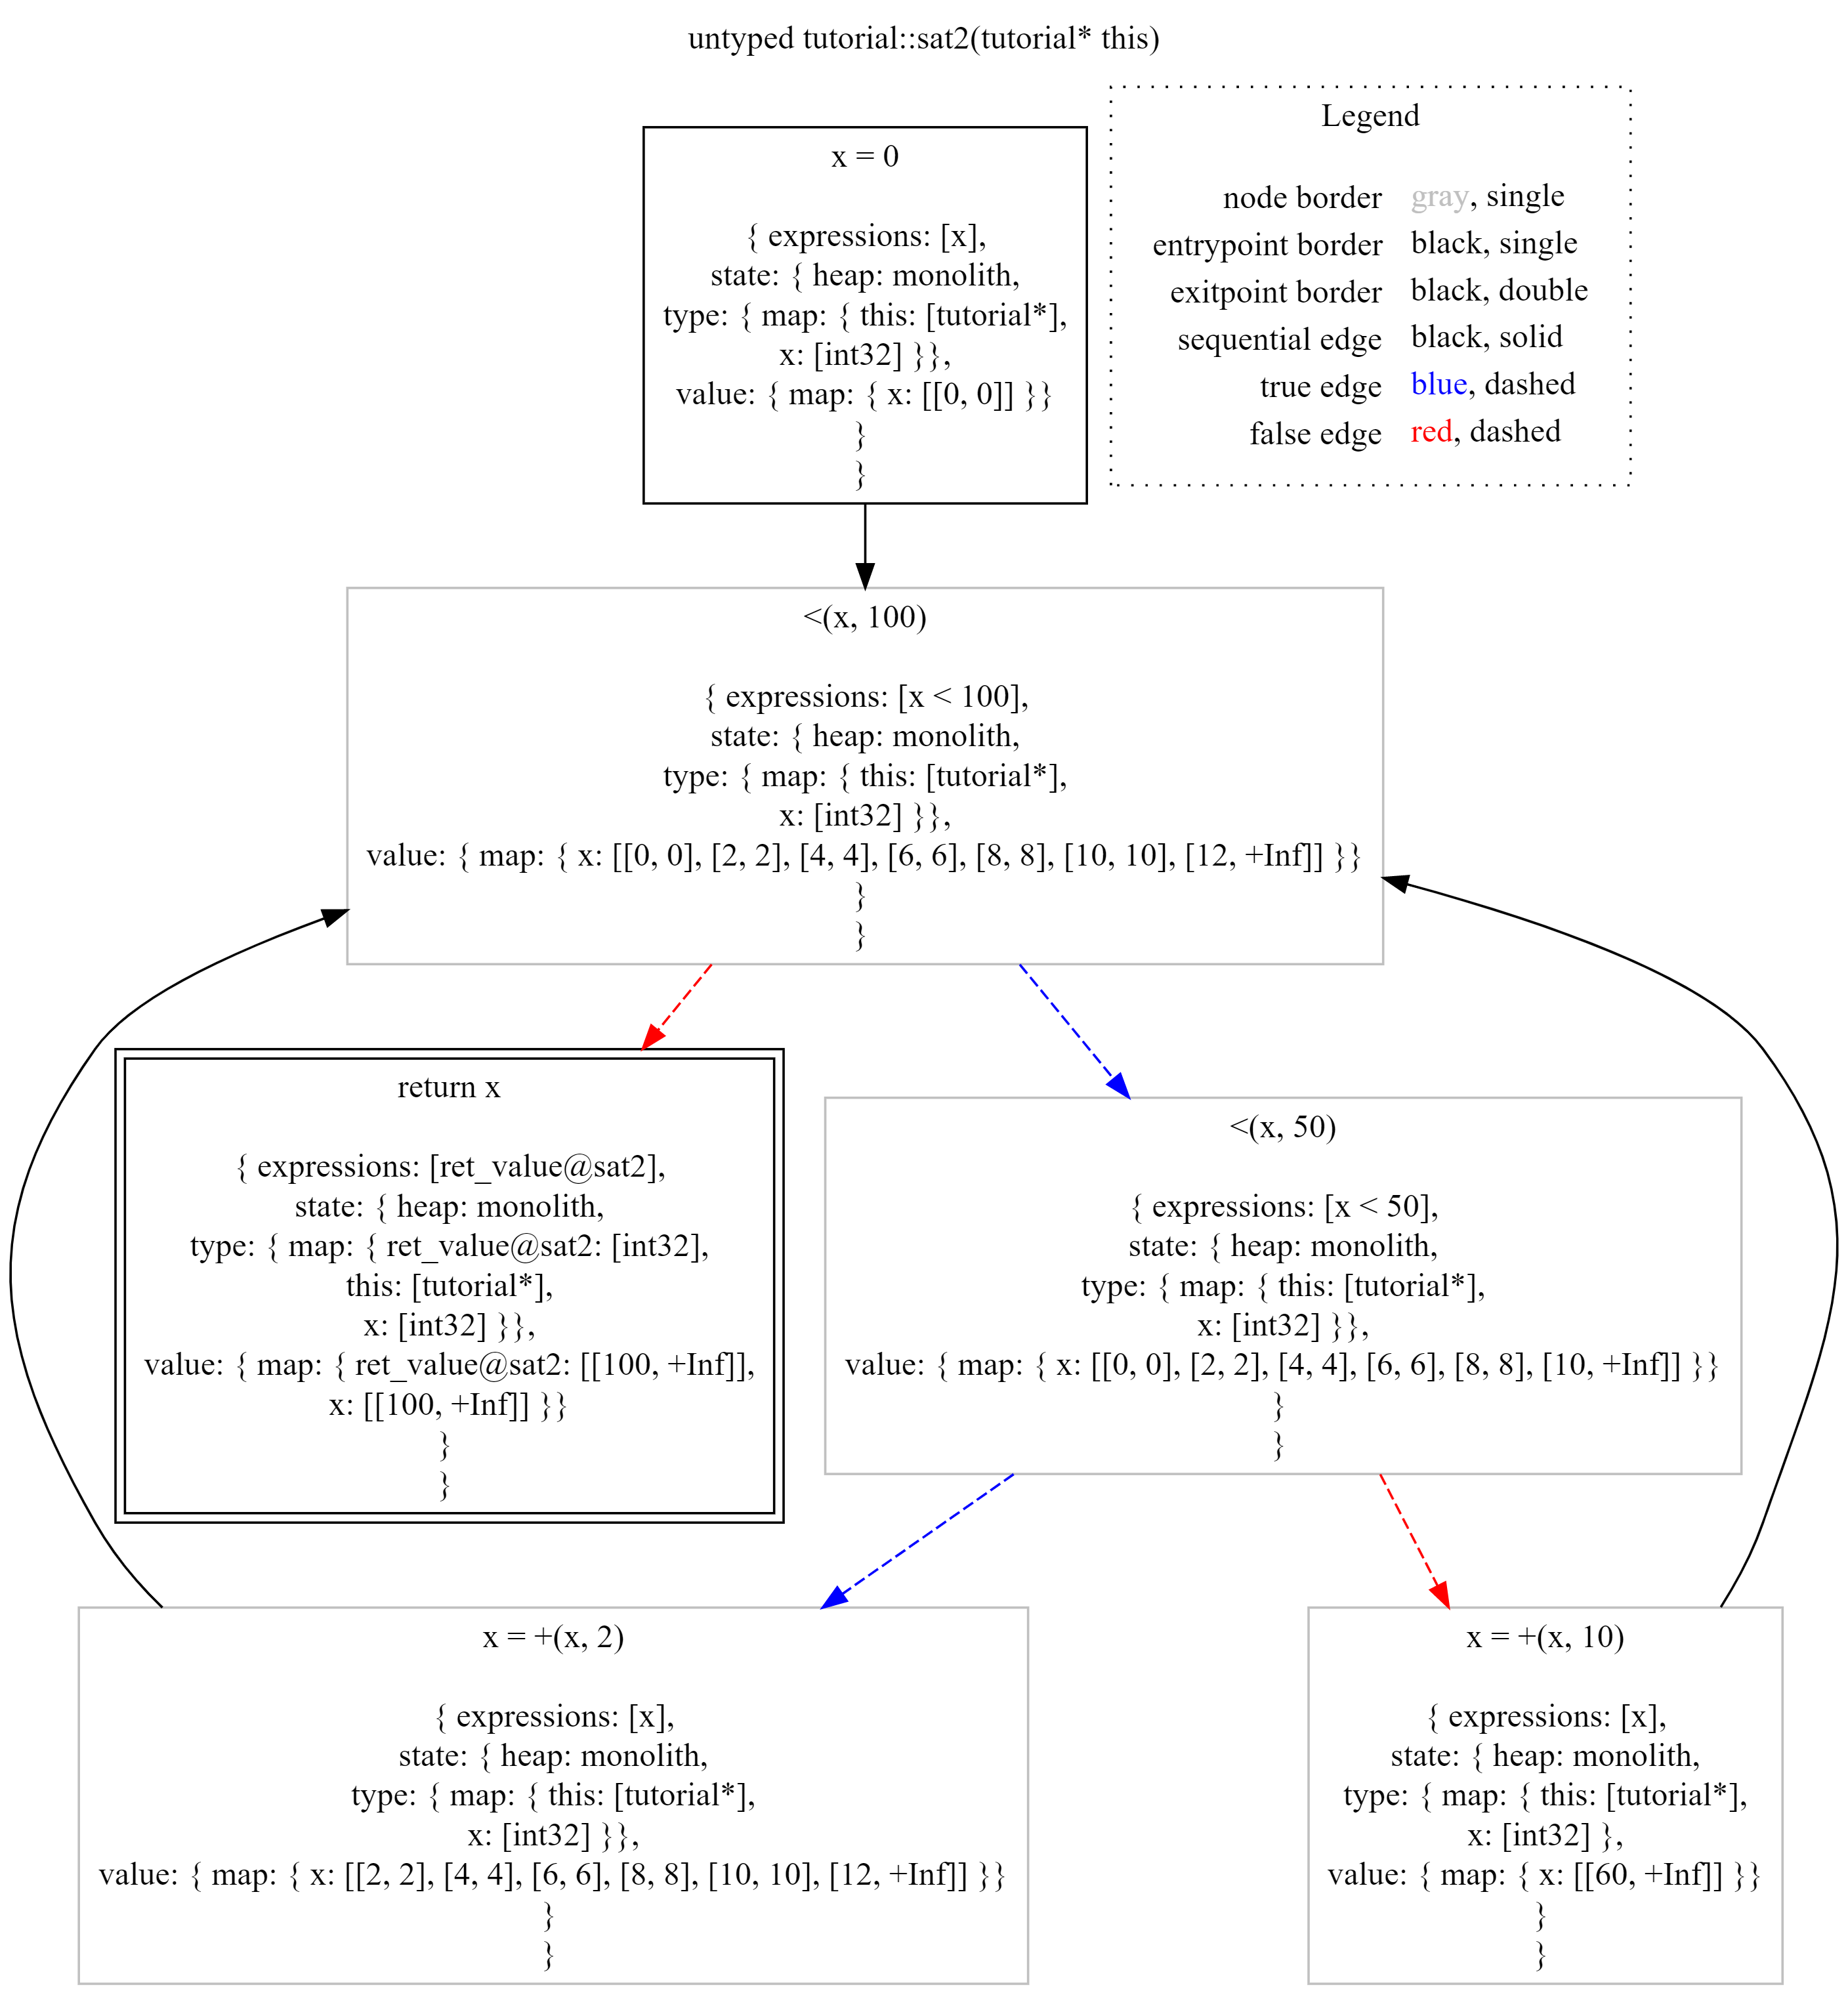
\includegraphics[width=0.7\textwidth]{Immagini/graphvizAscPowerset.png}
	\caption{Risultato in formato DOT dell'analisi del programma nella Figura \ref{fig:codiceEsempio2} con il dominio non relazionale dei sottoinsiemi non ridondanti di \texttt{Interval}.}
	\label{fig:risultatoAscPowerset}
\end{figure}

\section{La fase discendente in LiSA}\label{sec:descendingLiSA}
In questa sezione vedremo come è stata aggiunta in LiSA la possibilità di calcolare anche la fase discendente. Prima però di parlare delle modifiche apportate bisogna mostrare come effettivamente (quali classi e metodi sono utilizzati) è implementato il calcolo del fix-point di un programma in LiSA. Il flow che segue il calcolo è mostrato in figura \ref{fig:flowFixpoint}. 
\begin{figure}[ht]
	\centering
	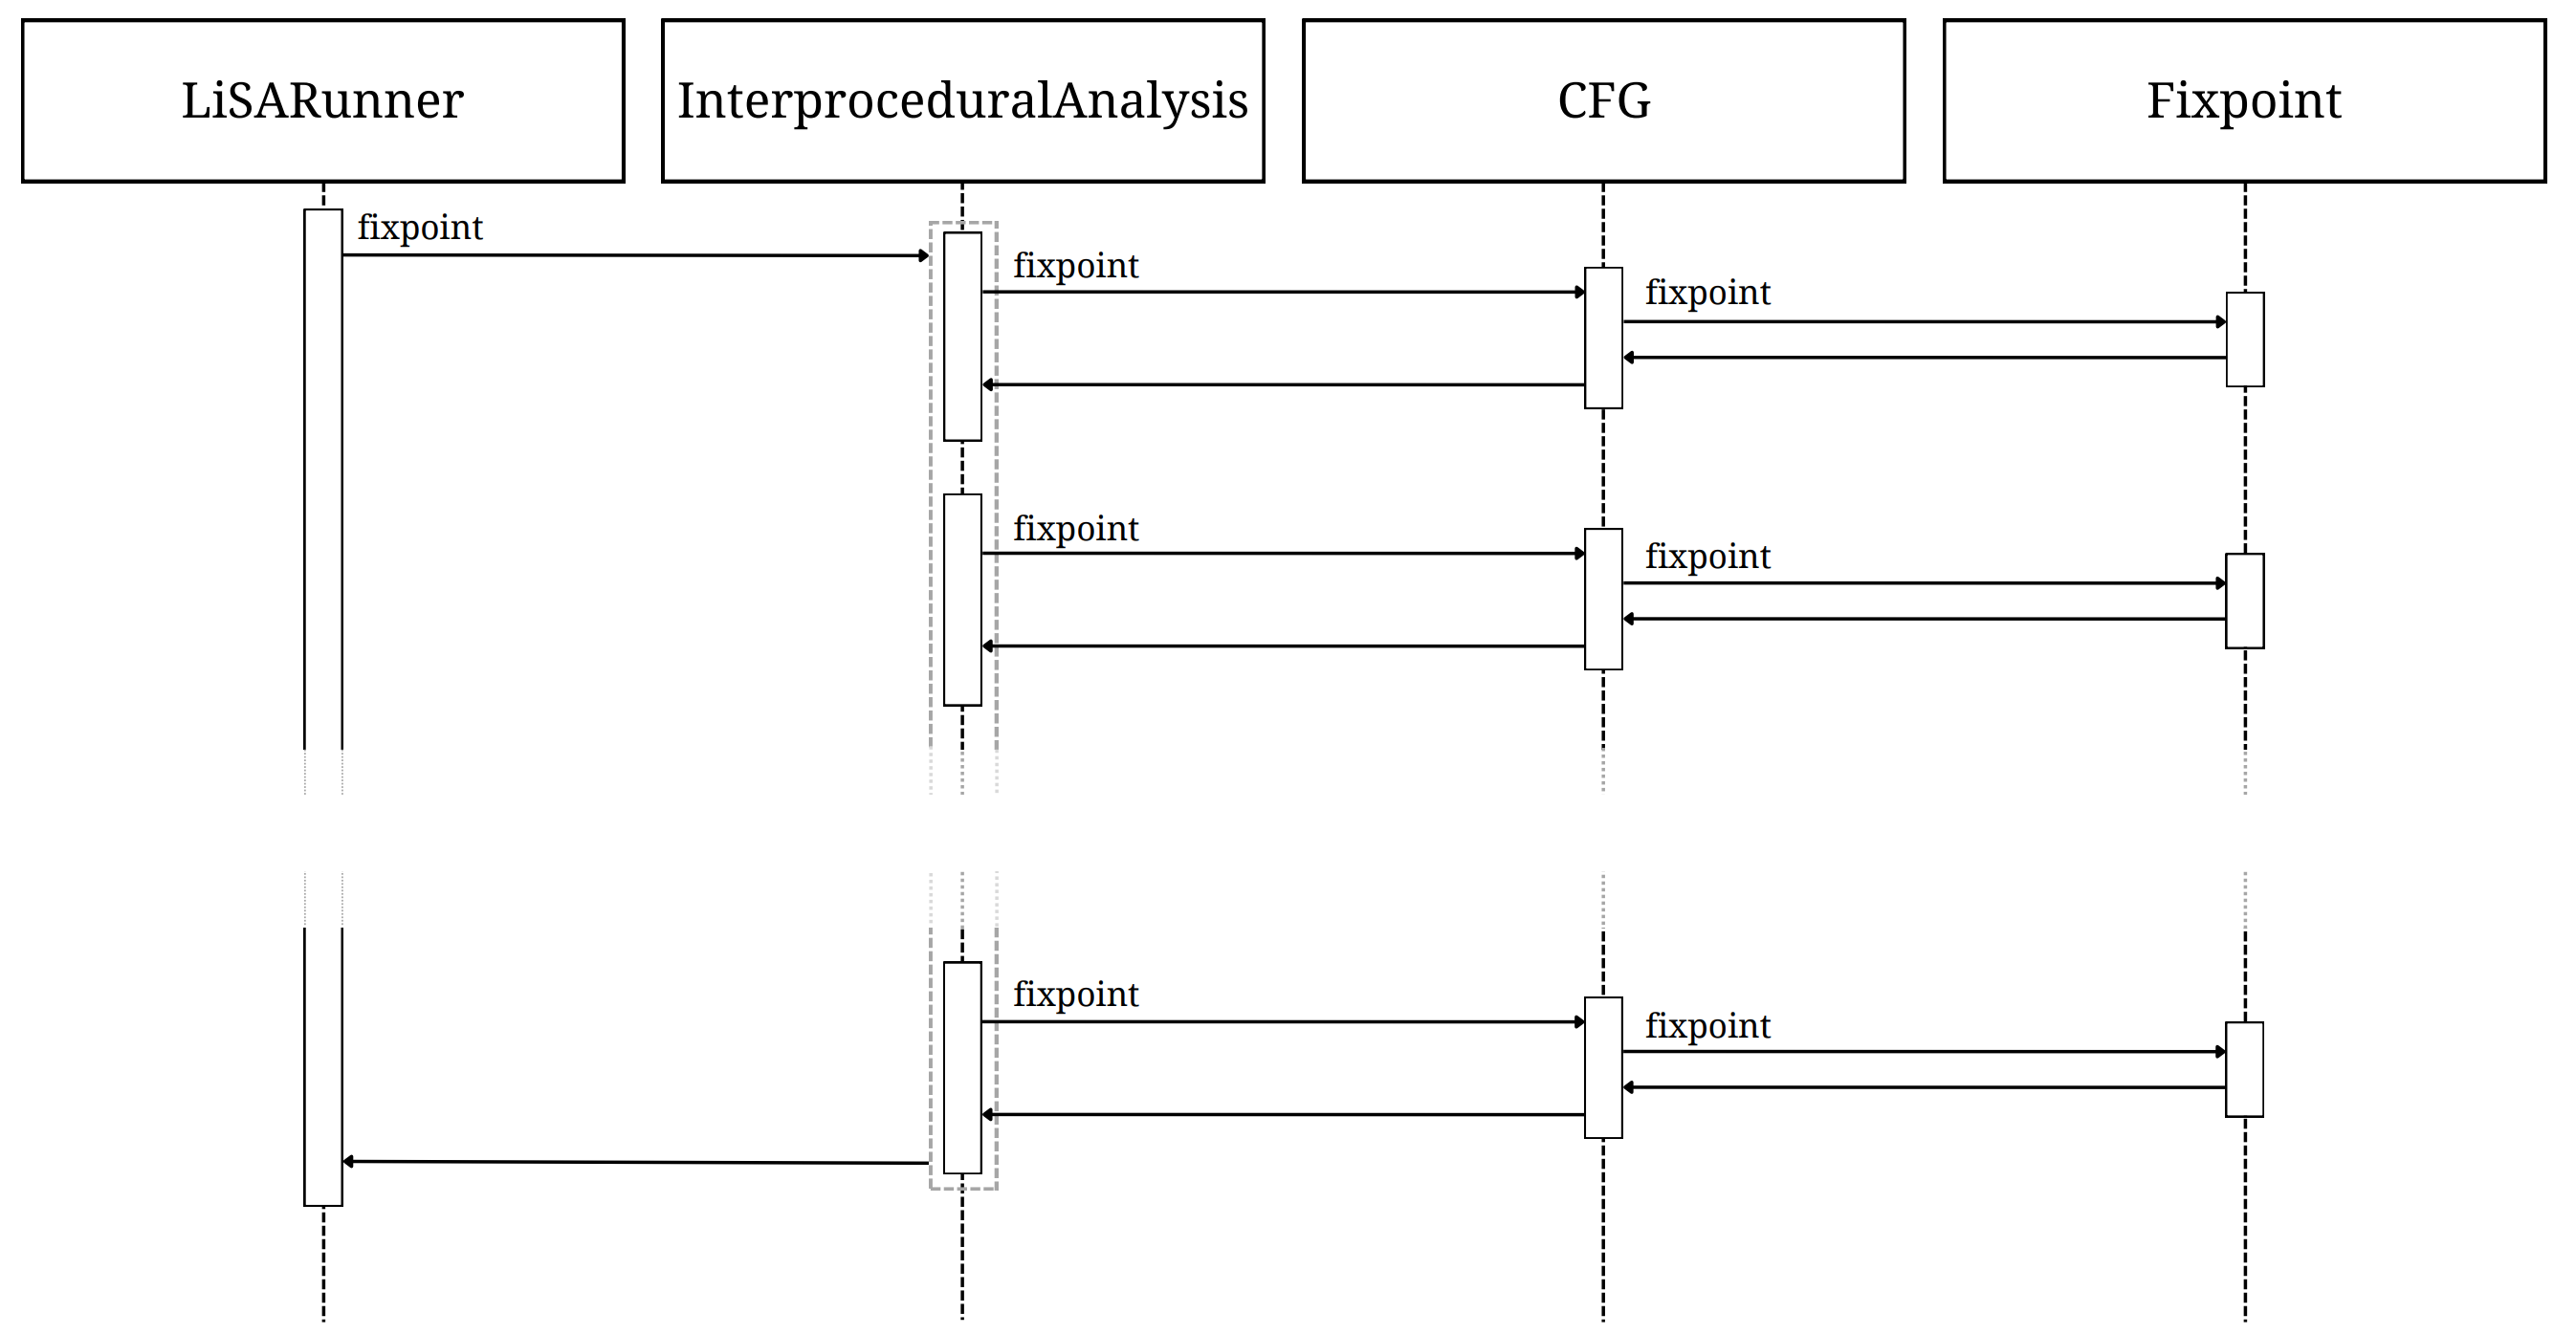
\includegraphics[width=\textwidth]{Immagini/flowFixpoint.png}
	\caption{Sequence diagram del calcolo del fixpoint.}
	\label{fig:flowFixpoint}
\end{figure}

\subsection{Il metodo \texttt{fixpoint} nelle diverse classi di LiSA}
Innanzitutto per ogni analisi bisogna scegliere una \texttt{InterproceduralAnalysys} che ha la visione completa del programma e delle sue unità (e quindi dei CFGs). L'interfaccia \texttt{InterproceduralAnalysys} ha un metodo \texttt{fixpoint} che quando viene chiamato deve calcolare il fix-point del programma (e quindi di ciascun CFG). Essendo il programma sotto analisi una collezione di CFG quello che effettivamente fa è iterare sull'insieme di CFG e uno a uno calcolare il suo fix-point. In LiSA i CFG sono oggetti della classe \texttt{CFG} che al suo interno definisce un metodo \texttt{fixpoint}, che appunto calcola il fix-point del CFG su cui viene chiamato (ed è il metodo chiamato dall'\texttt{InterproceduralAnalysis}). \texttt{CFG.fixpoint} non implementa però direttamente l'Algoritmo visto in \ref{alg:fixpointAsc}. Questo infatti viene implementatato in \texttt{Fixpoint.fixpoint} che in pratica è un blue-print per l'algoritmo del calcolo del fix-point tramite working-set list. Qui di seguito è mostrata la sua implementazione (leggermente semplificata) prima delle modifiche per includere la fase discendente. 
\begin{lstlisting}[belowskip=-1.1 \baselineskip, escapechar=|]
public Map<N, T> fixpoint(
        Map<N, T> startingPoints,
        WorkingSet<N> ws,
        FixpointImplementation<N, E, T> imp) {

    result = Map<N, T>();
    startingPoints.keySet().forEach(ws::push);

    T newApprox;
    while (!ws.isEmpty()) {
        N current = ws.pop();

        T entrystate = |\textcolor{deepgreen}{getEntryState}|(current, result, imp);
        newApprox = |\textcolor{deepyellow}{imp.semantics}|(current, entrystate);

        T oldApprox = result.get(current);
        newApprox = |\textcolor{deepyellow}{imp.join}|(current, newApprox, oldApprox);

        if (!|\textcolor{deepyellow}{imp.equality}|(current, newApprox, oldApprox)) {
            result.put(current, newApprox);
            for (N instr : graph.followersOf(current))
                ws.push(instr);
        }
    }
    return result;
}

private T |\textcolor{deepgreen}{getEntryState}|(
        N current,
        Map<N, T> result,
        FixpointImplementation<N, E, T> imp){
    
    Collection<N> preds = graph.predecessorsOf(current);
    List<T> states = new List<T>();

    for (N pred : preds) {
        if (result.containsKey(pred)) {
            E edge = graph.getEdgeConnecting(pred, current);
            states.add(|\textcolor{deepyellow}{imp.traverse}|(edge, result.get(pred)));
        }
    }

    T entrystate = null;
    for (T state : states)
        entrystate = |\textcolor{deepyellow}{imp.union}|(current, entrystate, state);

    return entrystate;
}
\end{lstlisting}
Come si può vedere tutte le operazioni principali (evidenziate in giallo) sono delegate all'oggetto \texttt{imp} che implementa l'interfaccia \texttt{FixpointImplementation}. Questa interfaccia dichiara i seguenti metodi:
\begin{itemize}
\itemsep0pt
    \item \texttt{T semantics(N node, T entrystate)}: deve modificare il pre-state applicando la funzione semantica dello statement rappresentato dal nodo;
	\item \texttt{T traverse(E edge, T entrystate)} : applica il significato semantico dell'arco al post-state di un nodo;
	\item \texttt{T union(N node, T left, T right)} : unisce i post-state dei nodi precedenti al corrente passati attraverso il significato semantico dell'arco che li unisce (operazione compiuta da \texttt{traverse});
	\item \texttt{T join(N node, T approx, T old)} : viene utilizzato per fare il join tra gli step delle iterazioni del sistema di equazioni. All'interno di questo viene scelto se usare il lub o il widening;
	\item \texttt{boolean equality(N node, T approx, T old)} : ci dice se la nuova approssimazione è minore od uguale a quella vecchia, e quindi se dobbiamo o no propagare nuove informazioni nei nodi successivi;
\end{itemize}
Questa interfaccia è implementata all'interno della classe \texttt{CFG} dalla classe \texttt{CFGFixpointImplementation}. Questa definisce tutti metodi elencati sopra (per esempio definisce la logica della scelta tra lub e widening tramite threshold). Un'oggetto di questa classe viene creato con i dovuti parametri di configurazione (ad esempio il threshold per il widening) prima della chiamata a \texttt{fixpoint} di \texttt{Fixpoint} e poi passato ad esso.

Il metodo così definito \texttt{Fixpoint.fixpoint} sarebbe quasi perfetto anche per la fase discendente tranne che per tre differenze:
\begin{itemize}
\itemsep0pt
    \item non si dovrebbe iniziare da una mappa dei risultati vuota, ma dai risultati della fase ascendente;
    \item al posto del join dovrebbe essere fatto il meet tra gli step della iterazione;
    \item il metodo \texttt{equality} dovrebbe controllare che la nuova approssimazione sia maggiore od uguale a quella vecchia (ovvere dovrebbe fare il contrario rispetto a quello che fa durante la fase ascendente);
\end{itemize}
Per la questione dei risultati ho semplicemente aggiunto un parametro al metodo \texttt{Fixpoint.fixpoint} chiamato \texttt{initialResult} che è una mappa di risultati da cui partire. 
\begin{lstlisting}[belowskip=-1.1 \baselineskip, escapechar=|]
public Map<N, T> fixpoint(
        Map<N, T> startingPoints, 
        WorkingSet<N> ws,
        FixpointImplementation<N, E, T> imp, 
        Map<N, T> |\textcolor{deepblue}{initialResult}|){

    result = |\textcolor{deepblue}{initialResult}|;
    ...
}
\end{lstlisting}
A questo punto in \texttt{CFG.fixpoint} il metodo verrà chiamato due volte, la prima (fase ascendente) con una mappa di risultati vuota, la seconda (fase discendente) con i risultati della prima come mostrato nel piccolo schema della Figura \ref{fig:flowFaseDisc}.

Per gli altri due problemi (join/meet e metodo \texttt{equality}) è stato necessario avere un modo per tenere traccia di quale fase stessimo calcolando all'interno del \texttt{CFGFixpointImplmentation}. Ovvero un modo che ci dicesse che se siamo nella fase ascendente utilizziamo \texttt{join} con lub/widening ed \texttt{equality} con minore-uguale, se invece siamo nella fase discendente utilizziano \texttt{meet} con glb/narrowing ed \texttt{equality} con maggiore-uguale. Per correttezza sintattica inoltre ho dovuto cambiare la dichiarazione dell'interfaccia \texttt{FixpointImplementation} modificando il metodo \texttt{join} nel metodo \texttt{operation}. Sarà poi dentro la implementazione concreta di \texttt{operation} che il calcolo verrà smistato a \texttt{join} o \texttt{meet} a seconda della fase in cui ci si trova. Per tenere traccia della fase che sta calcolando ho aggiunto a \texttt{CFGFixpointImplementation} un parametro di configurazione di tipo \texttt{DescendingPhaseType}, che è così definito tramite un enum:  
\begin{lstlisting}[belowskip=-1.1 \baselineskip, escapechar=|]
public static enum DescendingPhaseType {

    NONE,
    
    GLB,
    
    NARROWING;
}
\end{lstlisting}
Se a \texttt{CFGFixpointImplementation} viene passato \texttt{DescendingPhaseType.NONE} supporrà di essere nella fase ascendente, se invece riceve \texttt{DescendingPhaseType.GLB} o \texttt{DescendingPhaseType.NARROWING} supporrà di essere in quella discendente. I tipi \texttt{GLB} e \texttt{NARROWING} indicano entrambi la fase discendente, ma con una diversa logica di scelta tra glb e narrowing durante l'esecuzione dell'operazione di meet (che dopo vedremo più nel dettaglio). A questo punto i metodi \texttt{equality} e \texttt{operation}, quando chiamati, controlleranno in quale fase si trovano e smisteranno il calcolo al metodo appropriato. Nella Figura \ref{fig:flowFaseDisc} è schematizzata la sequenza di chiamate di \texttt{CFG} a \texttt{Fixpoint}.

\begin{figure}
	\centering
	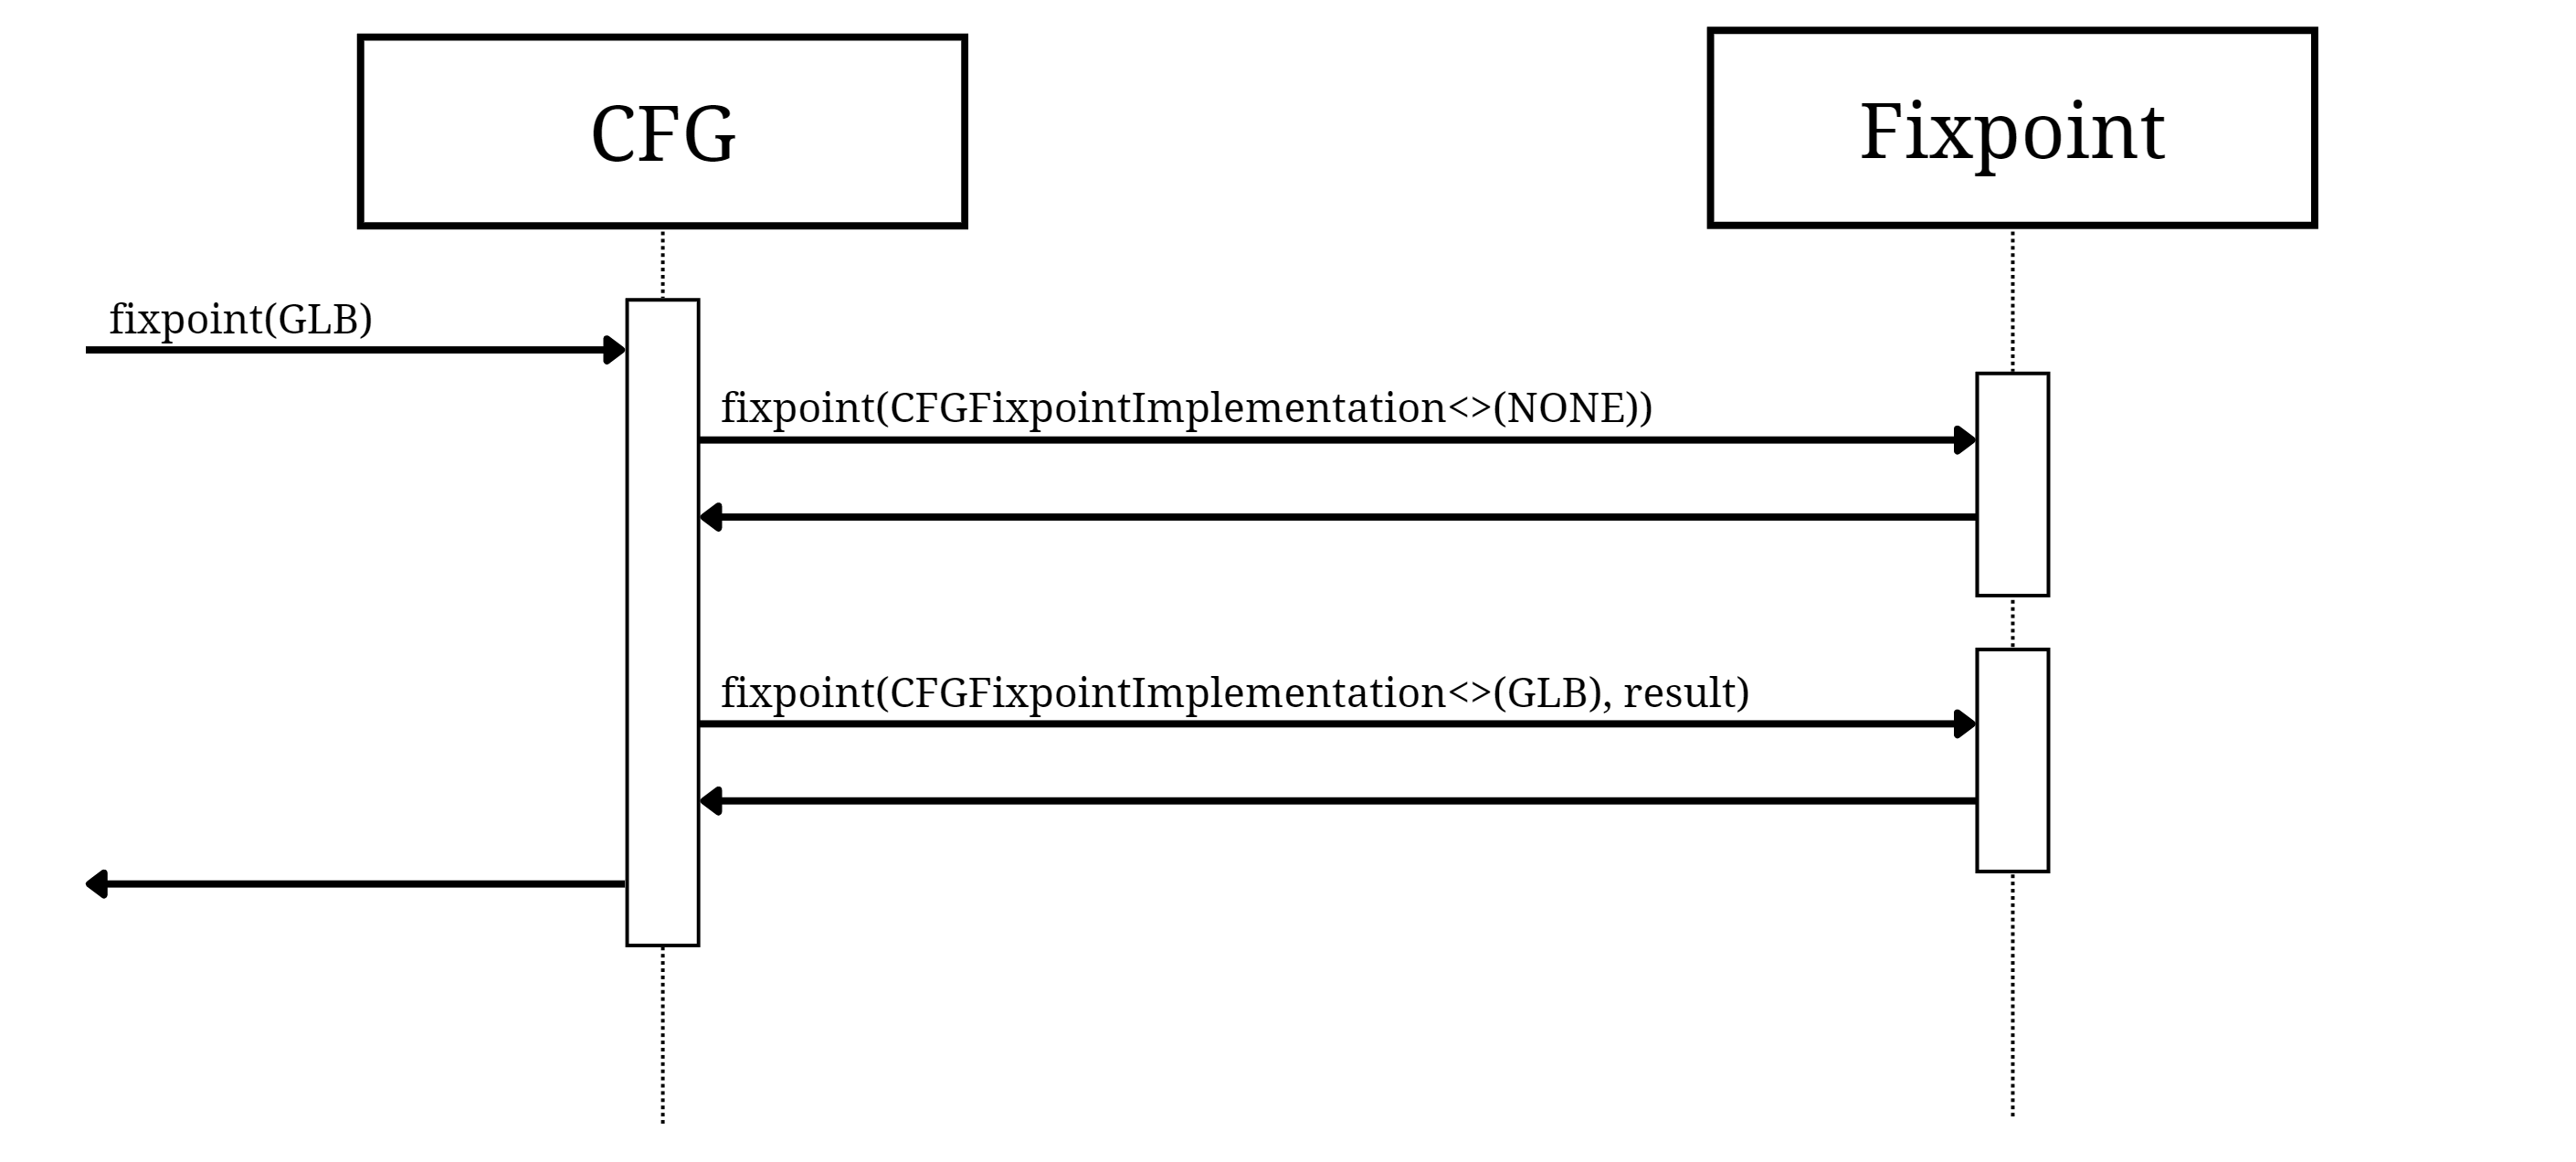
\includegraphics[width=0.9\textwidth]{Immagini/flowFaseDisc.png}
	\caption{Sequence diagram delle chiamata da \texttt{CFG} a \texttt{Fixpoint} dopo l'implementazione della fase discendente.}
	\label{fig:flowFaseDisc}
\end{figure}

\subsection{Il metodo \texttt{meet} in \texttt{CFGFixpointImplementation}}
In questa sezione guarderemo più nel dettaglio come è stata implementata l'operazione di meet utilizzata durante la fase discendente. Qui di seguito è mostrato il codice che lo definisce, dove per semplificare ho chiamto \texttt{T} il tipo dello stato astratto usato per l'analisi.  
\begin{lstlisting}[belowskip=-1.1 \baselineskip, escapechar=|]
public T meet(Statement node, T approx, T oldApprox){

    newApprox = approx;
    
    if (this.descendingPhase == DescendingPhaseType.NARROWING)
        newApprox = oldApprox.narrowing(newApprox);
    else if (this.descendingPhase == DescendingPhaseType.GLB){
        int glb = counter.computeIfAbsent(node, st -> threshold);
        if (glb > 0) 
            newApprox = newApprox.glb(oldApprox);
        else
            newApprox = oldApprox;
        counter.put(node, --glb);
    }
    return newApprox;
}
\end{lstlisting}
Sostanzialmente esistono due tipi di meet (o logiche per la scelta tra glb e narrowing) possibili in LiSA:
\begin{itemize}
\itemsep0pt
    \item \texttt{GLB}: utilizza un valore threshold passato come parametro di configurazione. In questa fase discendente viene utilizzato il glb come operatore di meet sempre fino a che non si passa per un nodo threshold volte, dopodichè non verrà fatta nessuna operazione e si ritornerà il valore della vecchia approssimazione. Così facendo siamo sicuri che dopo un numero finito di step si raggiunge un punto stazionario (e quindi la convergenza del calcolo);
    \item \texttt{NARROWING} : in questo caso come operatore viene sempre usato il narrowing. Anche in questo caso la convergenza è garantita se il narrowing dello stato astratto è definito con le caratteristiche mostrate nella Definizione \ref{def:narrowing};
\end{itemize}

A questo punto se vogliamo aggiungere il calcolo della fase discendente all'analisi mostrata nell'Esempio \ref{code:simpleAnalysisAsc} basterà aggiungere alla configurazione il tipo di fase discendente voluta ed i suoi eventuali parametri, come mostrato nell'esempio qui di seguito. 
\label{code:analisiDescending}
\begin{lstlisting}[belowskip=-1.1 \baselineskip]
LiSAConfiguration conf = new LiSAConfiguration();
conf.abstractState = LiSAFactory.getDefaultFor(
				AbstractState.class, 
				getDefaultFor(HeapDomain.class), 
				new Interval(),
				new TypeEnvironment<>(new InferredTypes()));
conf.wideningThreshold = 5;
conf.descendingPhaseType = DescendingPhaseType.GLB;
conf.descendingGlbThreshold = 5;
conf.analysisGraphs = GraphType.DOT;
conf.workdir = outputDirectory;
Program program = Frontend.processFile(programFilePath);
LiSA lisa = new LiSA(configuration);
lisa.run(program);
\end{lstlisting}
Se invece non si vuole che venga calcolata la fase discendente basta non settare il campo \texttt{descendingPhaseType} di \texttt{LiSAConfiguration}, che come default ha il valore \texttt{NONE}. Questo valore verrà passato duarante il flow del metodo \texttt{fixpoint} fino alla classe \texttt{CFG} che eviterà di fare la seconda chiamata a \texttt{Fixpoint.fixpoint} restituendo direttamente i risultati ottenuti dalla sola fase ascendente. Nella Figura \ref{fig:risultatoDOTDesc} è mostrato il risultato dell'analisi con anche la fase discendente del programma della Figura \ref{fig:codiceEsempio2} e le configurazioni mostrate sopra.
\begin{figure}[ht]
	\centering
	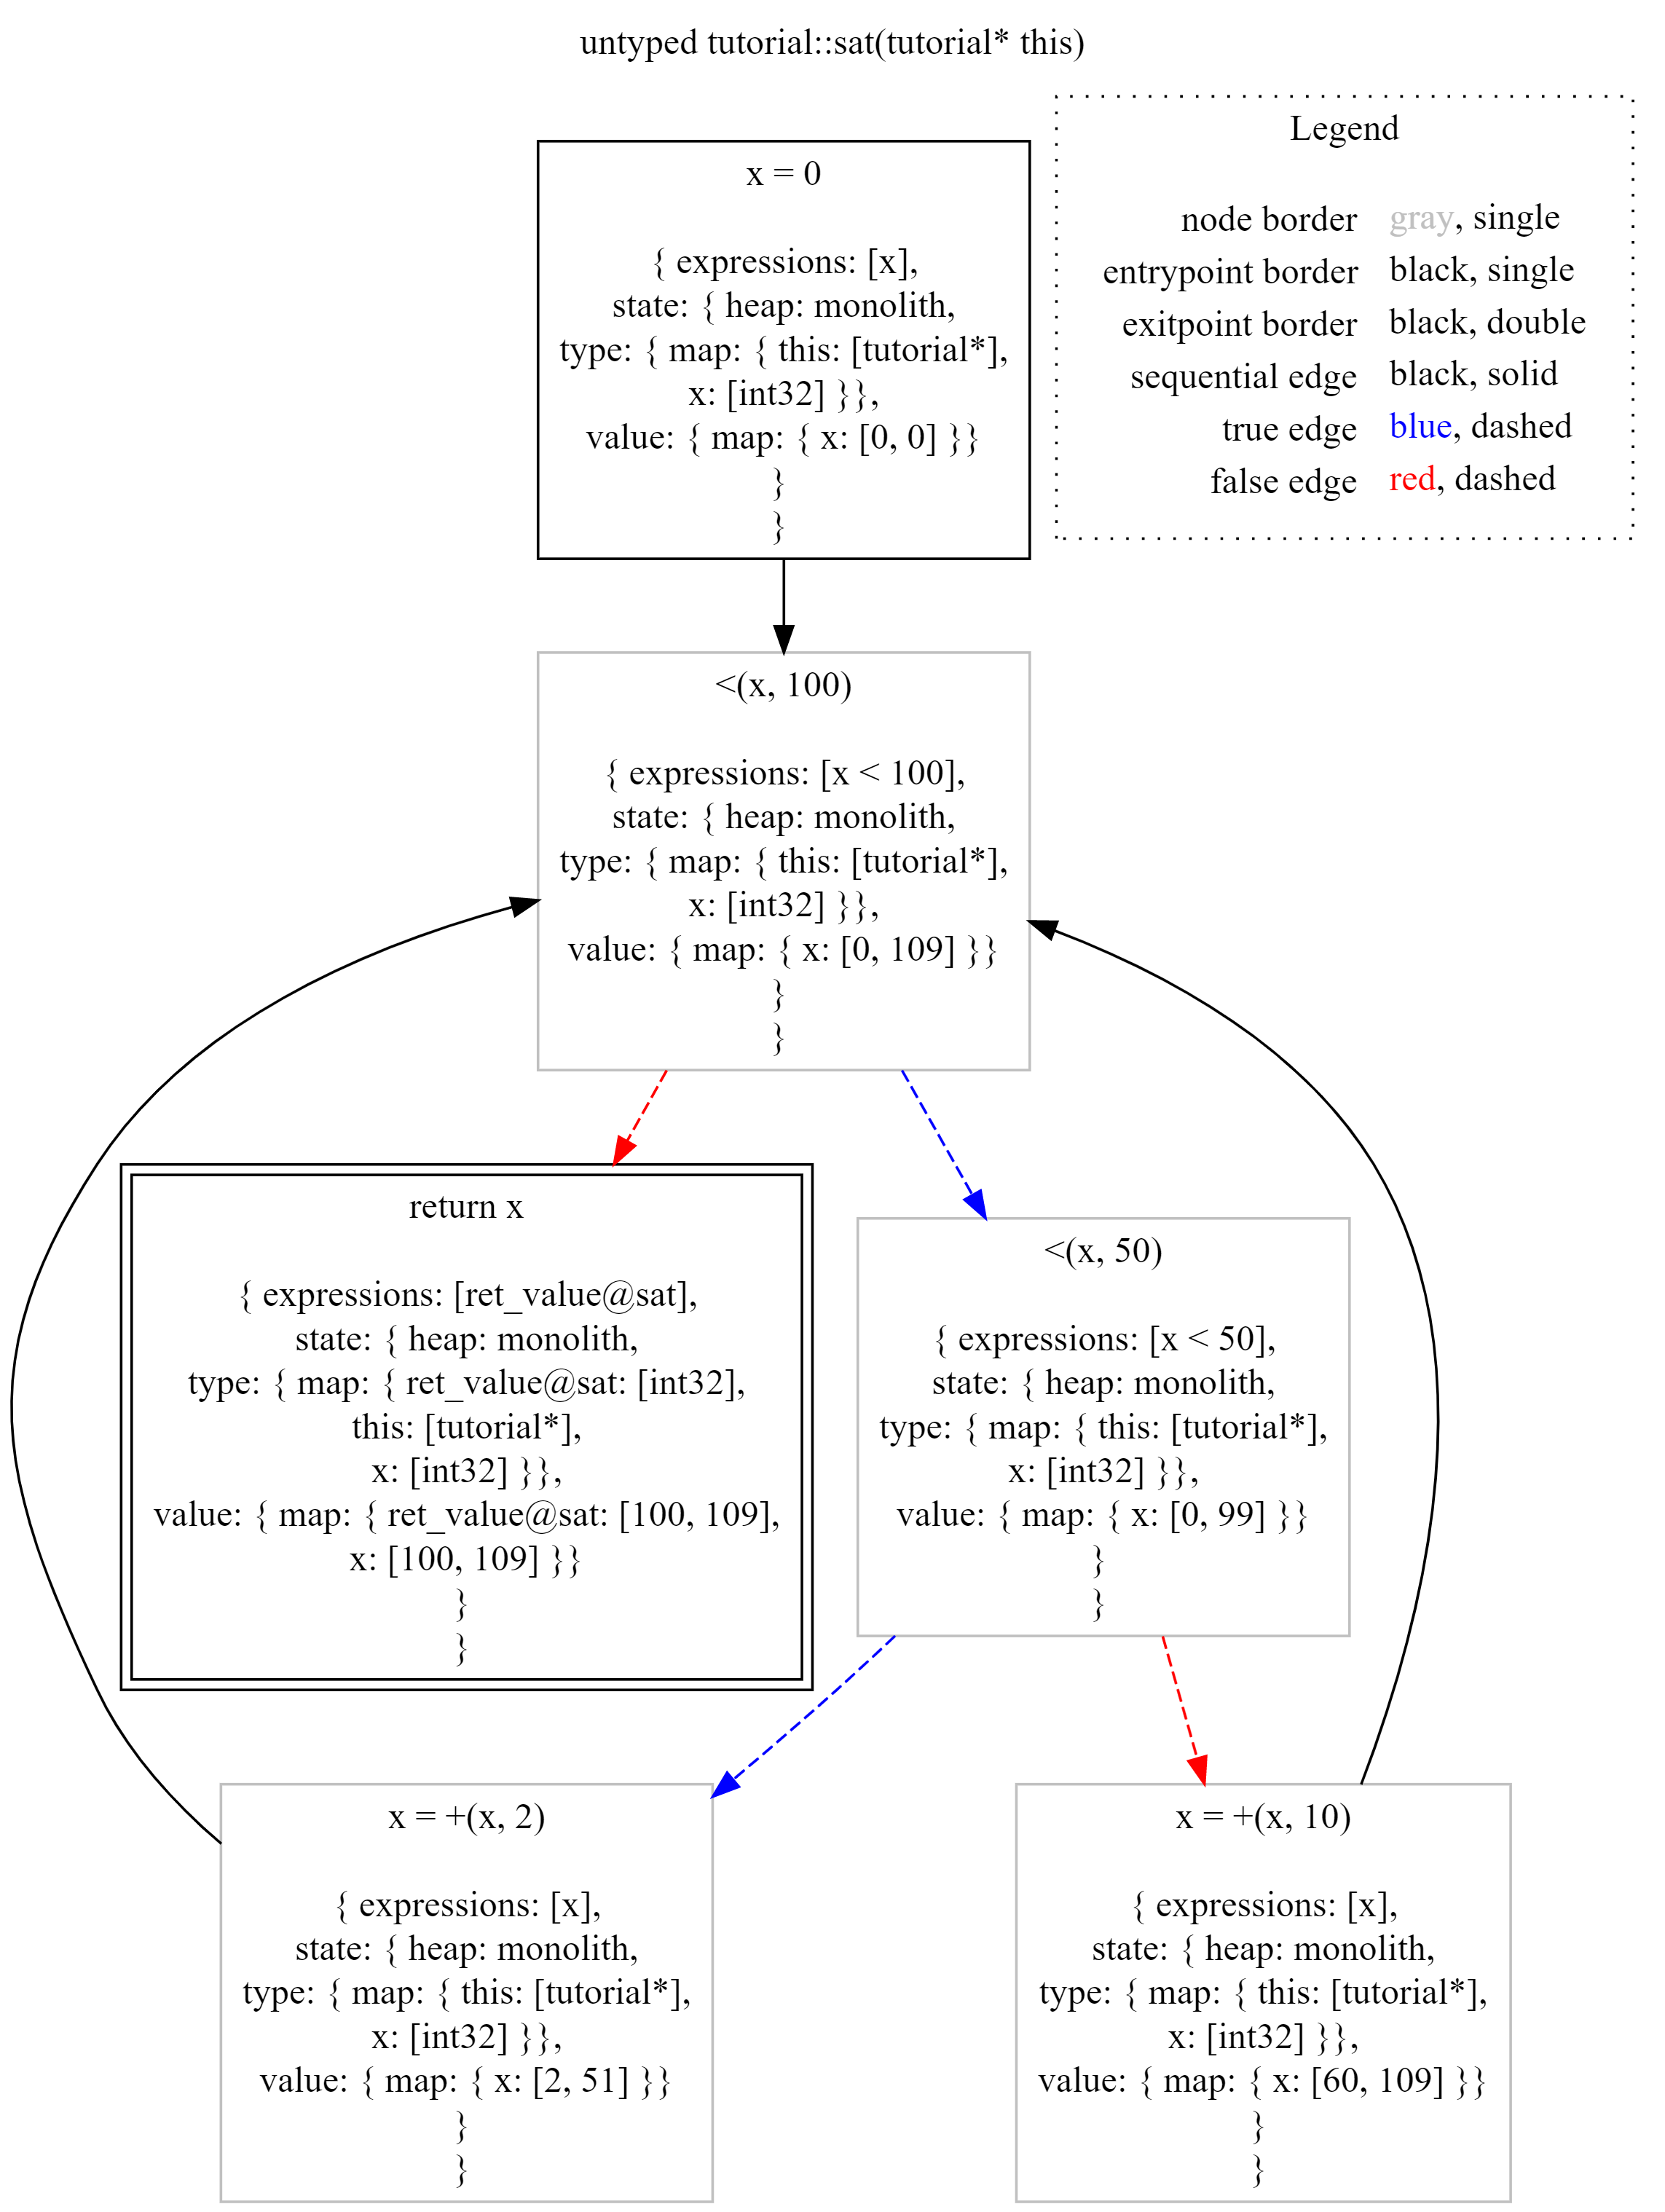
\includegraphics[width=0.8\textwidth]{Immagini/graphvizDesc.png}
	\caption{Risultato in formato DOT dell'analisi del programma \ref{fig:codiceEsempio2} con anche fase discendente.}
	\label{fig:risultatoDOTDesc}
\end{figure}

\section{Decoupling della fase ascendente e discendente in LiSA}\label{sec:lisaDecoupling}
In questa sezione vedremo come è stato possibile modificare LiSA per permettere il decoupling della fase ascendente e discendente come mostrato nel Capitolo \ref{chapter:decoupling}. Bisogna però dire che l'implementazione non è stata fatta per essere inserita ufficialmente dentro LiSA, ma come prova sperimentale per vedere realizzato in pratica il concetto e per fare qualche test. Anche per questo motivo non verrà data una spiegazione approfondita con estratti di codice come fatto in precedenza, ma solo una spiegazione generale del funzionamento e dell'architettura. Nella Figura \ref{fig:flowDecoupling} viene mostrato un sequence diagram che schematizza le chiamate e i passaggi che avvengono in LiSA durante una analisi con decoupling delle fasi. 
\begin{figure}[ht]
	\centering
	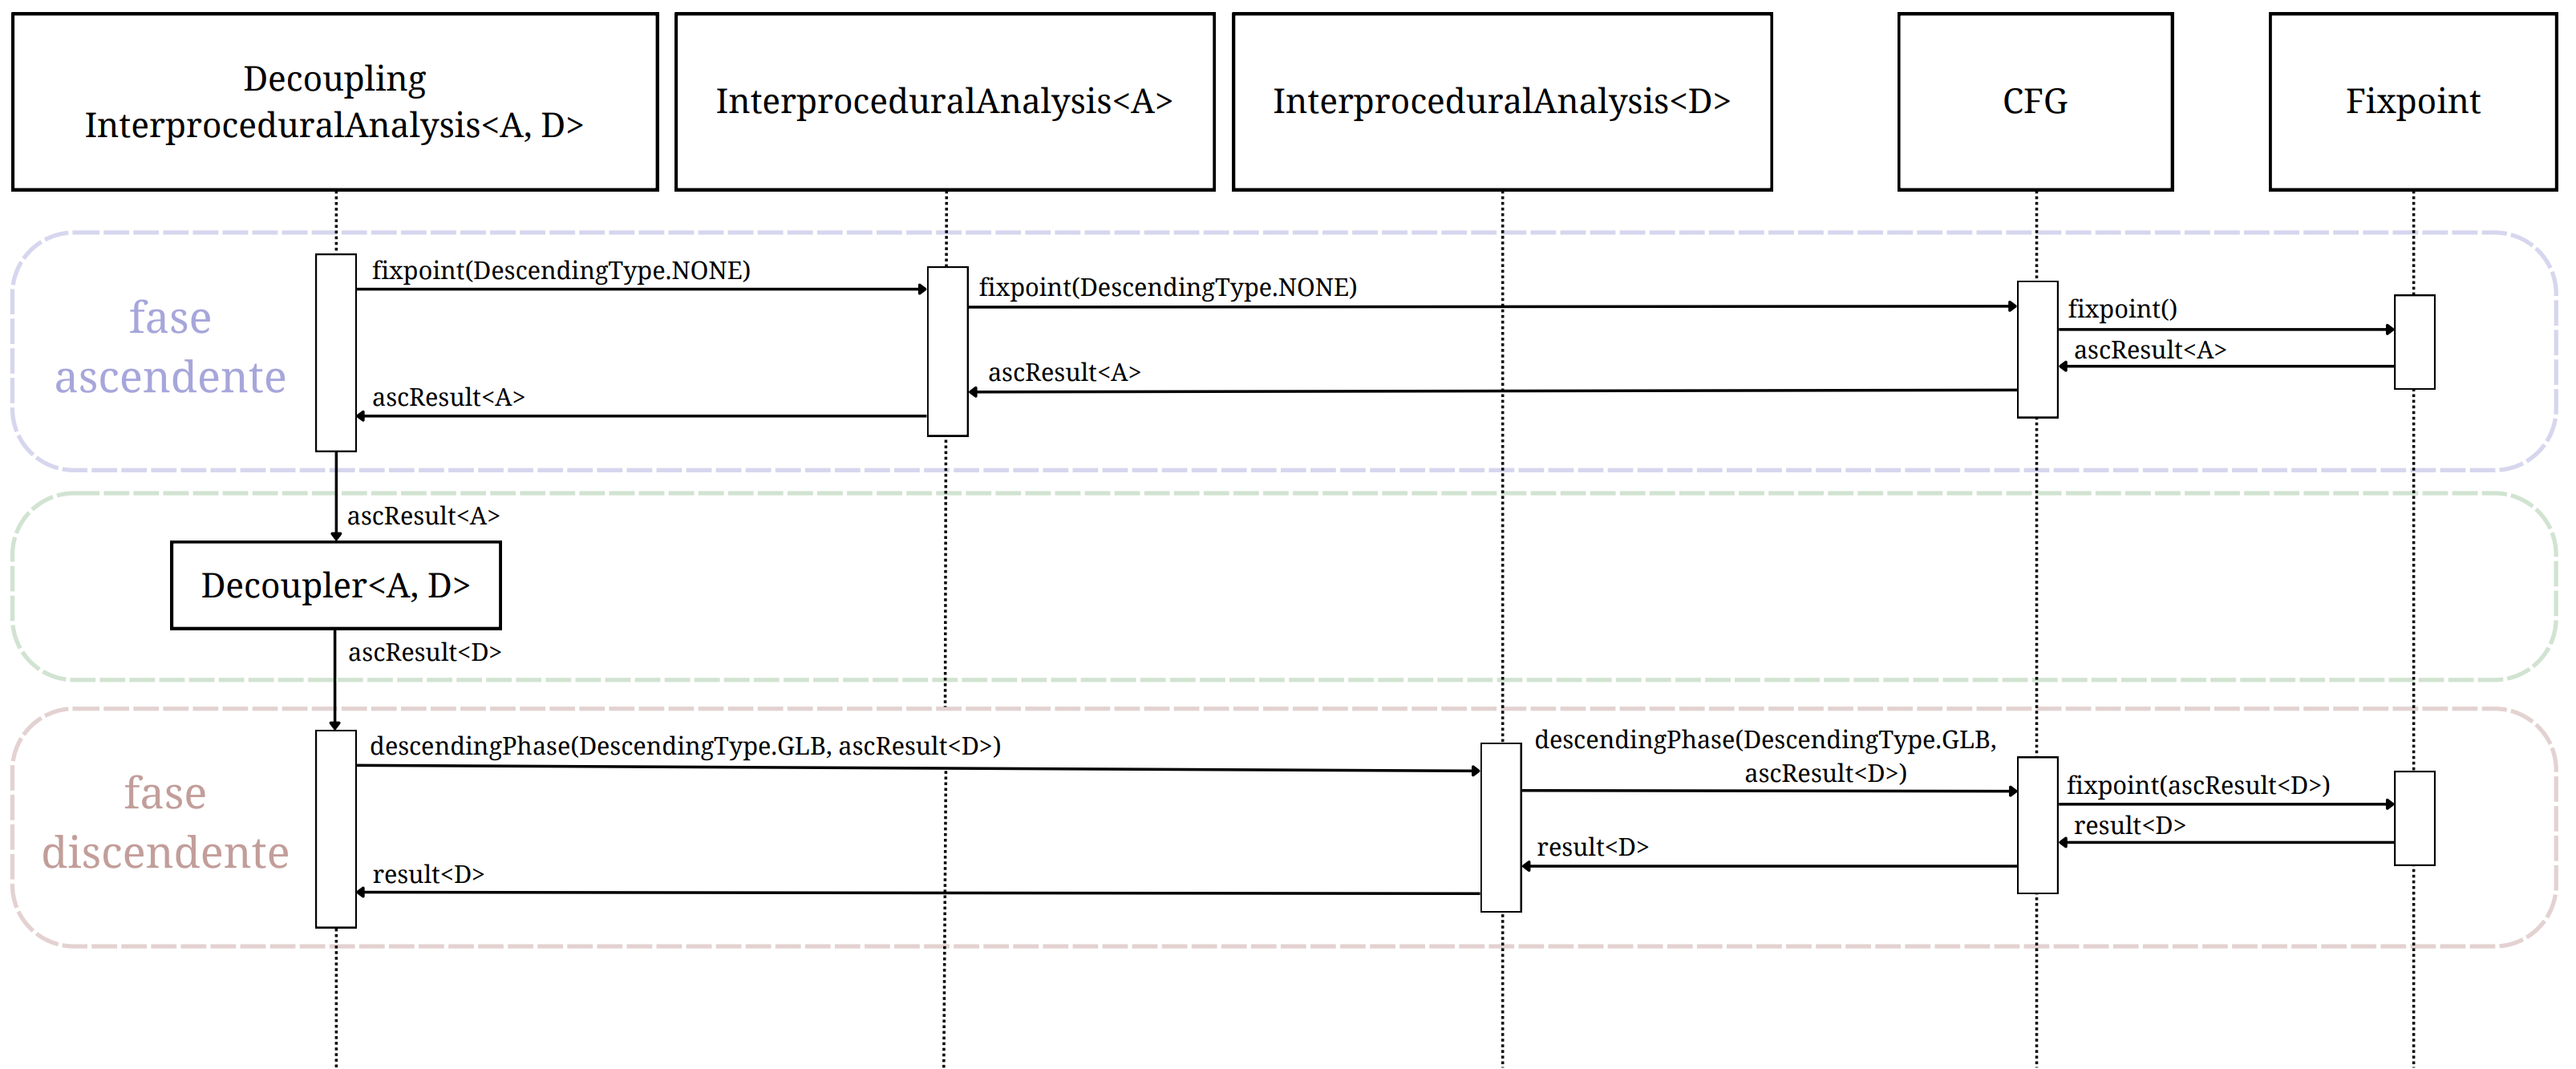
\includegraphics[width=\textwidth]{Immagini/decouplingFlow.png}
	\caption{Flow dell'analisi con decoupling delle fasi in LiSA.}
	\label{fig:flowDecoupling}
\end{figure}

Partiamo dal descrivere le componenti e i metodi aggiunti:
\begin{itemize}
\itemsep0pt
    \item \texttt{DecouplingInterproceduralAnalysis<A, D>}: è la \texttt{InterpoceduralAnalysis} da utilizzare per fare un'analisi con decoupling delle fasi. Incapsula al suo interno due \texttt{InterproceduralAnalysis} dello stesso tipo, una parametrica al tipo di stato astratto (che può essere considerato il dominio astratto) usato durante la fase ascendente, \texttt{A}, e una parametrica allo stato astratto usato durante la fase discendente, \texttt{D}. 
    \item \texttt{Decoupler<A, D>}: è l'oggetto che si occupa della traduzione da un dominio all'altro. \'E capace quindi di trasformare l'\texttt{AbstractState<A>} utilizzato nella fase ascendente nell'\texttt{AbstractState<D>} usato in quello discendente. Questo oggetto deve essere progettato ad-hoc per ogni coppia di \texttt{A} e \texttt{D}. 
    \item è poi stato poi aggiunto il metodo \texttt{descendingPhase(DescendingPhaseType, ascResult<D>)} alle classi \texttt{InterproceduralAnalysis} e \texttt{CFG}. Questo metodo si occupa di calcolare la sola fase discendente partendo dai risultati della fase ascendente tradotti nel dominio astratto discendente.
\end{itemize}
La sequenza di operazioni è la seguente:
\begin{enumerate}
\itemsep0pt
    \item viene chiamato il metodo \texttt{fixpoint} sull'oggetto di tipo \texttt{DecouplingInterproceduralAnalysis<A, D>};
    \item \texttt{DecouplingInterproceduralAnalysis<A, D>} chiama \texttt{fixpoint} sulla \texttt{InterproceduralAnalysis<A>}, dicendogli di calcolare solamente la fase ascendente. I risultati ottenuti sono nel tipo del dominio astratto ascendente \texttt{A};
    \item i risultati della fase ascendente vengono tradotti dal \texttt{Decoupler} nel dominio astratto discendente, così da poter essere usati come punto di partenza per la fase discendente;
    \item \texttt{DecouplingInterproceduralAnalysis<A, D>} chiama \texttt{descendingPhase} sulla \texttt{InterproceduralAnalysis<D>} passando il tipo di fase discendente e il risultato della fase ascendente tradotto;
\end{enumerate}
Il seguente frammento di codice descrive quello che deve essere aggiunto a quello mostrato prima nell'Esempio \ref{code:analisiDescending} per applicare il decoupling delle fasi all'analisi. Più precisamente per usare il dominio \texttt{Sign} nella fase ascendente e \texttt{Interval} in quella discendente. 
\begin{lstlisting}[belowskip=-1.1 \baselineskip]
LiSAConfiguration conf = new LiSAConfiguration();

SignToIntervalDecoupler decoupler = new SignToIntervalDecoupler<>();
decoupler.setStates(
        getDefaultFor(AbstractState.class, 
                        getDefaultFor(HeapDomain.class), 
                        new Sign(), 
                        new TypeEnvironment<>(new InferredTypes())), 
        getDefaultFor(AbstractState.class, 
                        getDefaultFor(HeapDomain.class), 
                        new Interval(), 
                        new TypeEnvironment<>(new InferredTypes())));

DecouplingModularWorstCaseAnalysisInterprocedural interproc = 
    new DecouplingModularWorstCaseAnalysisInterprocedural<>(
    decoupler);

conf.interproceduralAnalysis = interproc;
//.....
lisa.run(program);
\end{lstlisting}
I risultati dell'analisi sono mostrati in Figura \ref{fig:risultatoDecoup}.
\begin{figure}[ht]
	\centering
	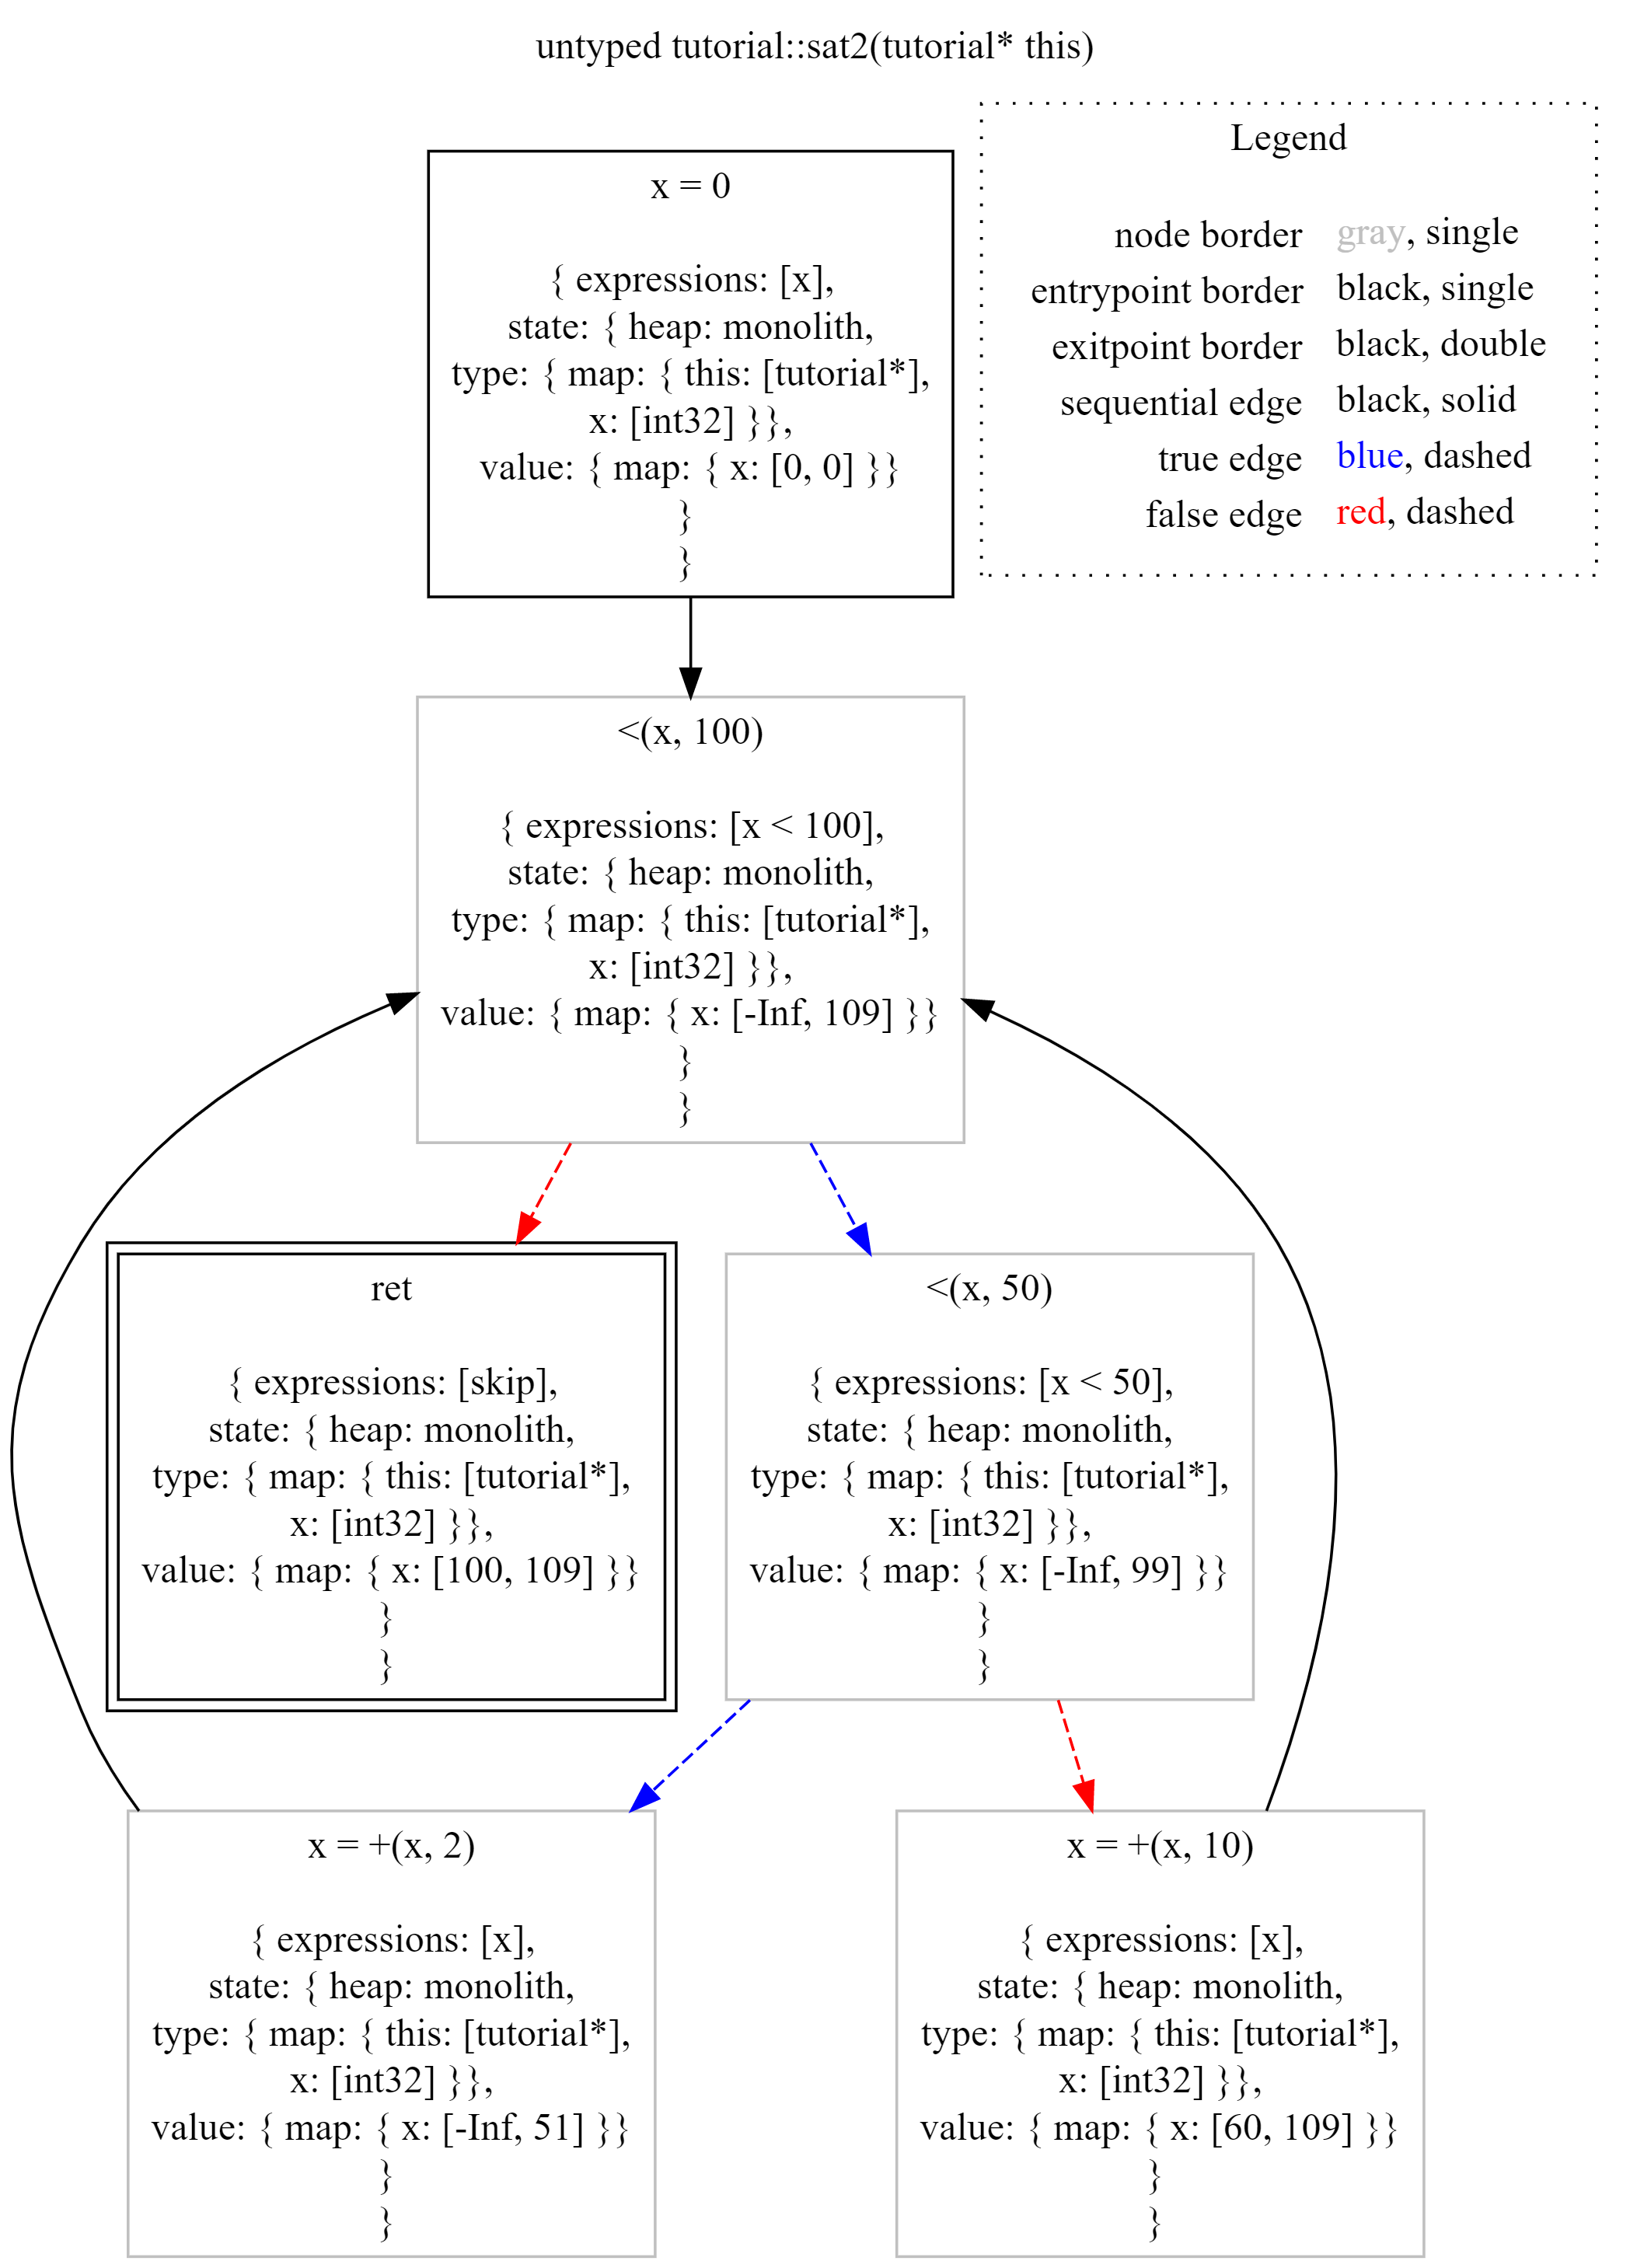
\includegraphics[width=0.7\textwidth]{Immagini/graphvizDecoup.png}
	\caption{Risultato in formato DOT dell'analisi del programma \ref{fig:codiceEsempio2} con anche fase discendente disaccoppiata da quella ascendente.}
	\label{fig:risultatoDecoup}
\end{figure}


%\chapter{Risultati}\label{chapter:res}
\Blindtext %Dummy Text - remove
%
%
%%%% Le Conclusioni
%\pagestyle{plain}
\chapter*{Conclusione} %Se si cambia il Titolo cambiare anche la riga successiva così che appia corretto nell'conclusione
\addcontentsline{toc}{chapter}{Conclusione} %Per far apparire Introduzione nell'indice (Il nome deve rispecchiare quello del chapter)
Conclusione che riassume il lavoro svolto ed eventuali lavori futuri.

\blindtext %Dummy Text - remove
\blindtext %Dummy Text - remove
%
%%%% La bibliografia
\bibliographystyle{apalike} %{plain} -- Scegliere lo stile preferito
\bibliography{./Bibliografia}
%
%\chapter*{Ringraziamenti}

%
% Le appendici
%\appendix
%\chapter{Appendice di Esempio}
\Blindtext
%
\end{document}